
\documentclass[11pt,openright,twoside,a4paper]{report}

% Defining aliases
\newcommand{\detection}{Detection}%{Block Detection and Pose Estimation}
\newcommand{\analysis}{Analysis}%{Reconstruction and Analysis}
\newcommand{\display}{Visualisation}%{Visualisation and Variation}
\newcommand{\jenga}{Jenga\textsuperscript{\textregistered{}}}
\newcommand{\mytitle}{\textbf{An Augmented Reality Variation of \jenga{}}}
\newcommand\todo[1]{\textcolor{red}{#1}}
%\renewcommand\todo[1]{}
\newcommand\nameandsecref[1]{\nameref{#1} (\cref{#1})}

\usepackage{xstring}
\usepackage{enumitem}
\usepackage{xifthen}
\usepackage{comment}
\usepackage{csquotes}
\usepackage{wrapfig}


\newcommand\blockwidth{0.8}
\newcommand\blockheight{\the\numexpr\blockwidth*3/5}
\newcommand\blockseparation{0.1}

\newcommand{\drawblockrow}[4]{
    \begin{tikzpicture}
        \draw[rounded corners] (0, 0) rectangle (\the\numexpr\blockwidth*3+\blockseparation*2, \the\numexpr\blockheight) {};
        
        \ifthenelse{\isempty{#1}}{}{\draw[rounded corners] (0, \the\numexpr\blockheight+\blockseparation) rectangle (\the\numexpr\blockwidth, \the\numexpr\blockheight*2+\blockseparation) {};}
        
        \ifthenelse{\isempty{#2}}{}{\draw[rounded corners] (\the\numexpr\blockwidth+\blockseparation, \the\numexpr\blockheight+\blockseparation) rectangle (\the\numexpr\blockwidth*2+\blockseparation, \the\numexpr\blockheight*2+\blockseparation) {};}
        
        \ifthenelse{\isempty{#3}}{}{\draw[rounded corners] (\the\numexpr\blockwidth*2+\blockseparation*2, \the\numexpr\blockheight+\blockseparation) rectangle (\the\numexpr\blockwidth*3+\blockseparation*2, \the\numexpr\blockheight*2+\blockseparation) {};}
        
        \draw[rounded corners] (0, \the\numexpr\blockheight*2+\blockseparation*2) rectangle (\the\numexpr\blockwidth*3+\blockseparation*2, \the\numexpr\blockheight*3+\blockseparation*2) {};
        
        \IfEqCase{#4}{%
        {1}{
            \draw[red] (0, \the\numexpr\blockheight+\blockseparation) -- (\the\numexpr\blockwidth, \the\numexpr\blockheight*2+\blockseparation);
            \draw[red] (0, \the\numexpr\blockheight*2+\blockseparation) -- (\the\numexpr\blockwidth, \the\numexpr\blockheight+\blockseparation);
        }
        {2}{
            \draw[red] (\the\numexpr\blockwidth+\blockseparation, \the\numexpr\blockheight+\blockseparation) -- (\the\numexpr\blockwidth*2+\blockseparation, \the\numexpr\blockheight*2+\blockseparation);
            \draw[red] (\the\numexpr\blockwidth+\blockseparation, \the\numexpr\blockheight*2+\blockseparation) -- (\the\numexpr\blockwidth*2+\blockseparation, \the\numexpr\blockheight+\blockseparation);
        }
        {3}{
            \draw[red] (\the\numexpr\blockwidth*2+\blockseparation*2, \the\numexpr\blockheight+\blockseparation) -- (\the\numexpr\blockwidth*3+\blockseparation*2, \the\numexpr\blockheight*2+\blockseparation);
            \draw[red] (\the\numexpr\blockwidth*2+\blockseparation*2, \the\numexpr\blockheight*2+\blockseparation) -- (\the\numexpr\blockwidth*3+\blockseparation*2, \the\numexpr\blockheight+\blockseparation);
        }
    }
    \end{tikzpicture}
}

%%
%% Package includes to provide the basic style
%%
%\usepackage{harvard}    % Uses harvard style referencing
\usepackage{graphicx}   % Permits import of various graphics formats
\usepackage{hyperref}   % Provides hyperlinks to sections automatically
\usepackage{pdflscape}  % Provides landscape mode for end code listings
\usepackage{multicol}   % Provides ability to split output into columns
\usepackage{listings}   % Provides styled code listings

%%
%% Set some page size changes from the standard article class
%%
\usepackage[inner=4cm]{geometry}
%\usepackage{calc}
%\setlength{\parskip}{6pt}
%\setlength{\parindent}{0pt}
%\addtolength{\hoffset}{-0.5cm}
%\addtolength{\textwidth}{2.5cm}

%%
%% Format definitions for the style
%%





%\bibliographystyle{agsm}  %{alpha}
%\citationstyle{dcu}
\pagestyle{headings}
\fussy


%%
%% Definitions to provide layout in the dissertation title pages
%%
\newenvironment{spaced}[1]
  {\begin{minipage}[c]{\textwidth}\vspace{#1}}
  {\end{minipage}}


\newenvironment{centrespaced}[2]
  {\begin{center}\begin{minipage}[c]{#1}\vspace{#2}}
  {\end{minipage}\end{center}}


\newcommand{\declaration}[2]{
  \thispagestyle{empty}
  \begin{spaced}{4em}
    \begin{center}
      \LARGE\textbf{#1}
    \end{center}
  \end{spaced}
  \begin{spaced}{3em}
    \begin{center}
      Submitted by: #2
    \end{center}
  \end{spaced}
  \begin{spaced}{5em}
    \section*{COPYRIGHT}

    Attention is drawn to the fact that copyright of this dissertation rests
    with its author. The Intellectual Property Rights of the products
    produced as part of the project belong to the author unless otherwise specified
    below, in accordance with the University of Bath's policy on intellectual property 
   (see http://www.bath.ac.uk/ordinances/22.pdf).

    This copy of the dissertation has been supplied on condition that anyone
    who consults it is understood to recognise that its copyright rests with its
    author and that no quotation from the dissertation and no information
    derived from it may be published without the prior written consent of
    the author.

    \section*{Declaration}
    This dissertation is submitted to the University of Bath in accordance
    with the requirements of the degree of Bachelor of Science in the
    Department of Computer Science. No portion of the work in this dissertation
    has been submitted in support of an application for any other degree
    or qualification of this or any other university or institution of learning.
    Except where specifically acknowledged, it is the work of the author.
  \end{spaced}

  \begin{spaced}{5em}
    Signed:
  \end{spaced}
  }


\newcommand{\consultation}[1]{%
\thispagestyle{empty}
\begin{centrespaced}{0.8\textwidth}{0.4\textheight}
\ifnum #1 = 0
This dissertation may be made available for consultation within the
University Library and may be photocopied or lent to other libraries
for the purposes of consultation.
\else
This dissertation may not be consulted, photocopied or lent to other
libraries without the permission of the author for #1 
\ifnum #1 = 1
year
\else
years
\fi
from the date of submission of the dissertation.
\fi
\vspace{4em}

Signed:
\end{centrespaced}
}

%%
%% END OF DEFINITIONS
%%

% TODO notes
\usepackage[dvipsnames]{xcolor}

% for tables
\usepackage{booktabs}
%\usepackage[table,xcdraw]{xcolor}

% for references
\usepackage[noabbrev,capitalise,nameinlink]{cleveref}

\usepackage{subcaption} % used for multiple figures on same line
\usepackage{graphicx}
\graphicspath{ {./images/litreview/} }
\newcommand*{\doi}[1]{\href{https://doi.org/\detokenize{#1}}{doi: \detokenize{#1}}}

\hypersetup{
	colorlinks=true,       % false: boxed links; true: colored links
	linkcolor=blue,        % color of internal links
	citecolor=blue,        % color of links to bibliography
	filecolor=magenta,     % color of file links
	urlcolor=blue         
}

% for degrees symbol \degree
\usepackage{textcomp}
\usepackage{gensymb}

% for drawing arrows
\usepackage{tikz-cd}
\usepackage{tikz}
\usetikzlibrary{mindmap}


\usepackage{natbib}
\bibliographystyle{unsrtnat}
\setcitestyle{authoryear,open={(},close={)}}
\newcommand{\possessivecite}[1]{\citeauthor{#1}{\textcolor{blue}{'s}} (\citeyear{#1})}
\newcommand{\footurl}[2]{\href{#1}{#2}\footnote{\url{#1}}}


% Set this to the language you want to use in your code listings (if any)
\usepackage{bera}
\usepackage{times}

\lstset{
    breaklines,
    breakatwhitespace,
    basicstyle=\small,
    commentstyle=\color{OliveGreen},    % comment style
    escapeinside={\%*}{*)},          % if you want to add LaTeX within your code
    keywordstyle=\color{blue},       % keyword style
    stringstyle=\color{Mulberry},
    emphstyle=\color{Maroon},
    numbers=left,
    frame=single,
    tabsize=2
}

\lstdefinestyle{python}{
    language=python,
    emph={cv},
}

\lstdefinestyle{cpp}{
    language=c++,
    emph={cv,aruco,ucoslam,spdlog}
}

\lstdefinestyle{java}{
    language=java
}

% patch first line numbers
\usepackage{etoolbox}% http://ctan.org/pkg/etoolbox
\makeatletter
\patchcmd{\lst@GLI@}% <command>
  {\def\lst@firstline{#1\relax}}% <search>
  {\def\lst@firstline{#1\relax}\def\lst@firstnumber{#1\relax}}% <replace>
  {\typeout{listings firstnumber=firstline}}% <success>
  {\typeout{listings firstnumber not set}}% <failure>
\makeatother

% Mini table of contents
\usepackage{minitoc}

% Larger column separation
\setlength{\columnsep}{35pt}

\usepackage{wrapfig}
\title{\mytitle{}}
\author{Oliver Broomhall}
\date{Bachelor of Science in Computer Science with Honours\\The University of Bath\\May 2018}

\crefname{lstlisting}{listing}{listings}
\Crefname{lstlisting}{Listing}{Listings}
\crefname{enumi}{Requirement}{Requirements}
\begin{document}
\dominitoc
\setcounter{page}{0}
\pagenumbering{roman}

\maketitle\newpage
\consultation{0}\newpage
\declaration{\mytitle{}}{Oliver Broomhall}\newpage

\abstract
This paper proposes a novel approach to the \jenga{} analysis problem through the use of squared planar markers, physics simulation, and augmented reality. Current approaches in the area assume tower states with no rotational nor translational block movement, which is adequate for analysis in a lab environment, but not in the real world, where towers are subject to block misalignment. The solution put forward in this project not only provides the user with a robust structural integrity analysis, but also improves on state-of-the-art methods for block detection. Evaluation and testing show that this method can be extended for use with structures that are unlike the standard three-by-eighteen \jenga{} tower, provided they can be described using a library of predefined parts; proving the usefulness and potential for wider applications of the method.

\begin{figure}[p]
    \centering
    
\includegraphics[width=.5\linewidth]{images/qr}
    \caption{Video demonstration}
    \label{fig:demoqr}
\end{figure}
\newpage
\tableofcontents\newpage
\listoffigures\newpage

\chapter*{Acknowledgements}
A special thank you to the Charlotte and Julian from the Lovelace lab, without whom it would not have been possible to use the university's laser cutter.
\\\\
Also, a kind thank you to my project supervisor, Christian Richardt, for advice and support throughout.
\\\\
I would also like to mention my grandfather, John Reeves, for financial support and my close family for moral support throughout my time at the University of Bath.
%---=---==---===---====---=====---======---=====---====---===---==---=---%
%-                             INTRODUCTION                             -%
%---=---==---===---====---=====---======---=====---====---===---==---=---%

\chapter{Introduction}\label{chap:introduction}
\pagenumbering{arabic}

This introduction serves to give an insight into, and the \nameandsecref{sec:motivation} of, the \nameandsecref{sec:problem} that this paper aims to solve, and also present some \nameandsecref{sec:challenges} that are expected to be faced throughout.

\section{Motivation}\label{sec:motivation}

Augmented reality (AR) can be thought of as lying on \possessivecite{rvcontinuum} Reality-Virtuality (RV) continuum (\cref{fig:continuum}), which defines the transition between an environment consisting solely of real objects, and an environment consisting solely of virtual objects.  AR lies close to the real environment on the RV continuum, more specifically AR is the addition of virtual objects onto real objects. When discussing AR, people are usually referring to visual AR, however it is worth noting that can potentially apply to all senses, including hearing, touch, and smell \citep{aradvances}.

\begin{figure}[ht]
    \centering
    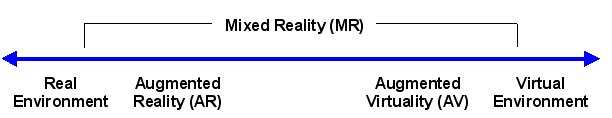
\includegraphics[width=0.8\textwidth]{images/proposal/RealityVirtualityContinuum}
    \caption{Simplified representation of a RV Continuum \protect\citep{rvcontinuum}.}
    \label{fig:continuum}
\end{figure}

Visual AR systems can be viewed through the use of projection displays, hand-held displays and head-worn displays. Some examples of head-worn displays currently in the market are shown in \cref{fig:headworndisplays}: Microsoft HoloLens, used for gaming and everyday applications such as video calling; Epson Moverio BT-300FPV Drone Edition, used for controlling a remote drone; and Google Glass Enterprise Edition, used to help businesses for activities like factory work and surgery. Smartphones and tablets can be used as hand-held displays, and are widely available as there are currently a predicted 2.53 billion smartphone users worldwide \citep{emarketer}. Uses for hand-held displays stretch from gaming and entertainment to training and education.

AR has recently gained popularity across many disciplines, and is estimated to explode in the coming years, as shown in \cref{fig:arstats}. A most notable area in AR is gaming, in which an AR smartphone game, Pokemon Go, hit a daily user count of 45 million, mere days after its release \citep{pokemongo}; an incredible achievement which was made possible through the use of new AR technology. It follows from these statistics that there is significant market potential in AR, specifically for AR in gaming.

\begin{figure}[ht]
\begin{minipage}{\textwidth}
\centering
\begin{minipage}{0.3\textwidth}
    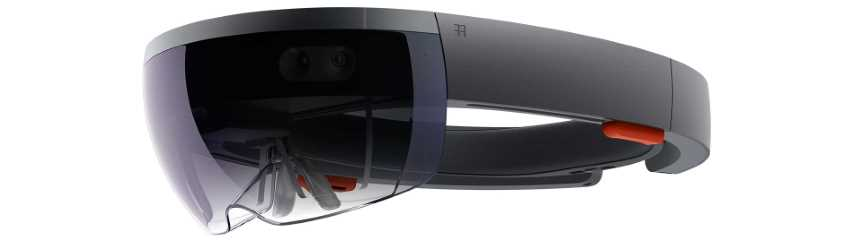
\includegraphics[width=\textwidth]{images/proposal/microsoft-hololens}
    \label{fig:hololens}
\end{minipage}\hfill
\begin{minipage}{0.3\textwidth}
    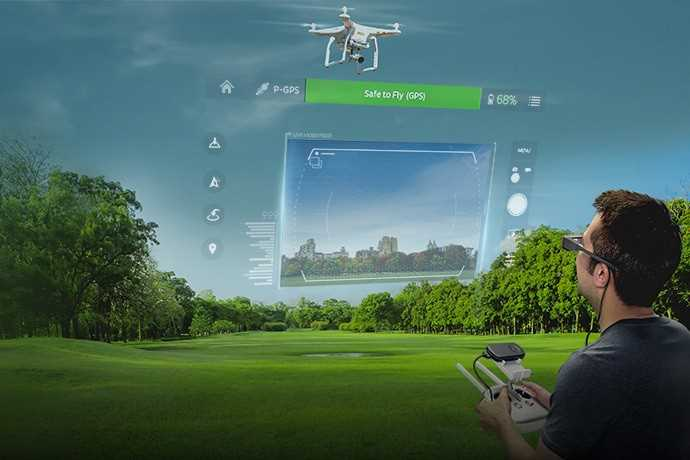
\includegraphics[width=\textwidth]{images/proposal/moverio-smart-glasses-2}
    \label{fig:epson}
\end{minipage}\hfill
\begin{minipage}{0.3\textwidth}
    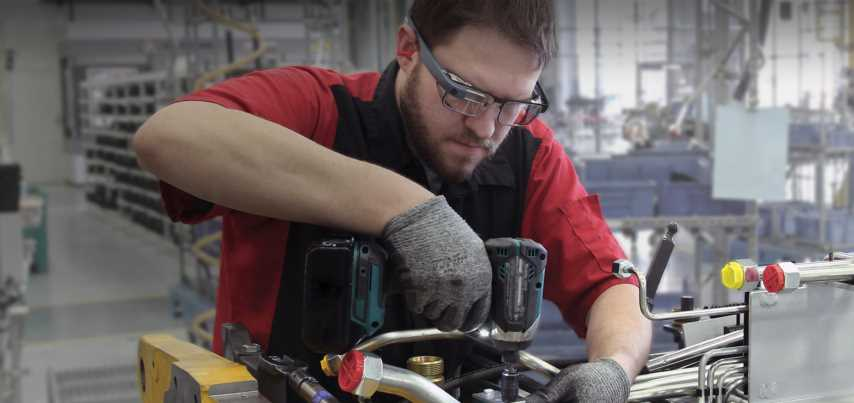
\includegraphics[width=\textwidth]{images/proposal/google-glass}
     \label{fig:glassee}
\end{minipage}
\caption{Current head-worn displays. \protect\footurl{https://www.microsoft.com/en-us/hololens}{Microsoft HoloLens} (left), \protect\footurl{https://epson.com/For-Home/Smart-Glasses/Smart-Glasses/Moverio-BT-300FPV-Smart-Glasses-\%28FPV-Drone-Edition\%29/p/V11H756020F}{Epson Moverio BT-300FPV Drone Edition} (centre), and \protect\footurl{https://x.company/glass/}{Google Glass} (right).}
\label{fig:headworndisplays}
\end{minipage}
\end{figure}

\begin{figure}[ht]
    \centering
    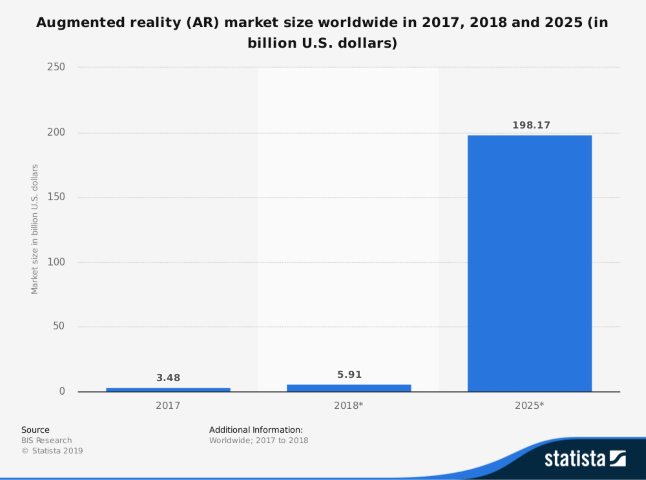
\includegraphics[width=0.65\linewidth]{images/proposal/statistic_id897587_augmented-reality-market-size-worldwide-2017-2025}
    \caption{Augmented reality (AR) market size worldwide in 2017, 2018 and 2025 (in billion U.S. dollars) \protect\citep{bisresearch}}
    \label{fig:arstats}
\end{figure}


%%
%
\section{Problem}\label{sec:problem}
%
%%

\jenga{} is a physical skill game that comprises of 54 wooden blocks, which begin, in a starting state, stacked in a tower of 3 block wide layers, with layers alternating between a 0\degree{} and 90\degree{} orientation. Players take turns in removing a block from the tower, and then placing that block on top of the tower, all whilst trying to prevent the tower from toppling over.

\begin{figure}[ht]
\begin{minipage}{\textwidth}
    \centering
    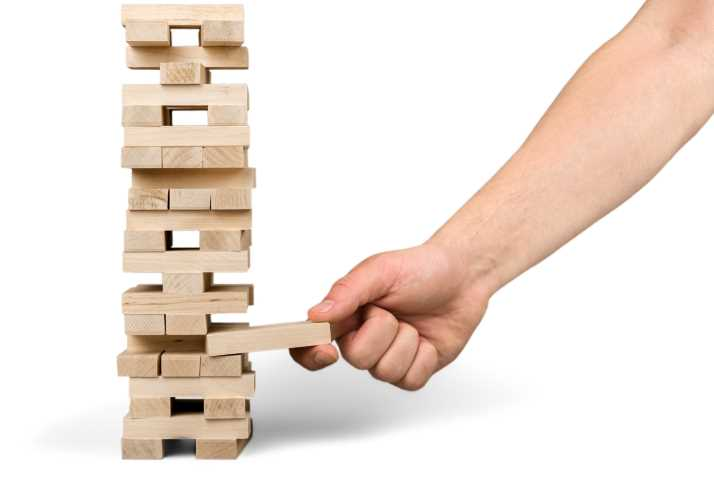
\includegraphics[width=0.5\linewidth]{images/proposal/jenga.jpeg}
    \caption{A \jenga{} tower obtained from \protect\footurl{https://stock.adobe.com/uk/}{Adobe Stock}}
    \label{fig:jenga}
\end{minipage}
\end{figure}

The main problem faced by players of \jenga{} is choosing which block to remove. Some variants even prevent the player from touching multiple blocks during their turn, thus they need to make a good decision before attempting block removal. Reasons to consider when deciding on the feasibility of removing a block depends on its situation in the tower, and can include: the block is supporting the structure above it, weighing down one side of the tower, is the last remaining in its layer, or is not easily accessible.

Several papers have addressed the aforementioned problem, some of which are discussed later in the \nameandsecref{chap:background}. However, current solutions rely on a fixed position camera, using a tripod, which would not be applicable in real instances of the game because players rarely have access to such camera equipment. In addition, previous projects which utilise the growing AR technology have all done so by creating a fully virtual tower in the starting state and adding that to the real environment. Furthermore, previous work done in the area also assume certain properties, such as alternating odd-even rows, and that blocks will be aligned to the shape of the tower.

This paper proposes a solution to the problem that allows for a more readily available free-moving camera, such as a smartphone. It also aims to make use of a real-world \jenga{} tower, which can be in any game state, meaning any number of player turns could have occurred before the system is first used, and also that individual blocks can be in any rotational or translational state. Doing this would improve significantly on the state-of-the-art technologies and research in the area.

The project spans over three crucial stages: firstly the detection of block poses, then an analysis of block removal feasibility, and finally result visualisation. In many sections of the report, it is deemed appropriate to treat the stages as separate entities that communicate by passing information between each other, and as such, the sections will retain a degree of modularity within this regard.

\section{Challenges} \label{sec:challenges}

Some challenges that may be faced in the undertaking of this project are detailed in the sections below:

As the solution aims to use real cameras, problems could arise due to the properties of each camera, such as image size and distortion. For example, if a camera is not calibrated to address distortion, then estimations of pose could be extremely inaccurate.

When using the system there may be times when the tower is not in-frame (visible by the camera), which could cause issues with false-positive detection. Furthermore, it may be difficult for the system to be able to distinguish between a block and a non-block gap in the tower because computer vision techniques need to be applied carefully to work well.

Reconstructing the tower for analysis may prove challenging as there may be inaccuracies in the detection of the blocks, as pose cannot be known, only estimated. In addition, finding a good method to analyse the block removal feasibility will be tough because accurately analysing real world physics is still an area of ongoing research in computer science.

Finally, as there are several ways to implement augmented reality in applications today, making it a troubling task to choose the right tool for displaying the results to the user.
Another item that needs to be considered is the creation of the user interface, with which ensuring usability is far from straightforward.

\section{Objectives}\label{objectives}

There are 3 objectives to work towards in this project, if all three objectives are met then the system is complete to the intended standard:

\begin{enumerate}
    \item\label{obj:detect} \textbf{Detect the poses of blocks in a real tower}
    \item\label{obj:analysis} \textbf{Analyse the removal feasibility of each block}
    \item\label{obj:display} \textbf{Visualise the results in an aesthetically pleasing manner}
\end{enumerate}

These objectives will be evaluated later on with a discussion into why they were, or indeed were not met by the end of the project.

Following this introduction, the paper will include; a \nameandsecref{chap:background} of the technologies used, capturing and setting project \nameandsecref{chap:requirements}, detailed \nameandsecref{chap:design} and \nameandsecref{chap:implementation}, all followed by a comprehensive \nameandsecref{chap:evaluation} and some thorough \nameandsecref{chap:conclusions}.




%---=---==---===---====---=====---======---=====---====---===---==---=---%
%-                          LITERATURE REVIEW                           -%
%---=---==---===---====---=====---======---=====---====---===---==---=---%

%++++++++++++++++++++++++++++++++++++++++++++++++++++++++++++++++++++++++++++++++++
%++++++++++++++++++++++++++++++++++++++++++++++++++++++++++++++++++++++++++++++++++
%++++++++++++++++++++++++++++++++++++++++++++++++++++++++++++++++++++++++++++++++++

\chapter{Background}\label{chap:background}

In this project there are three key milestones to be reached; constructing a virtual model from a real \jenga{} tower, using this construction to rank the feasibility of block removal, and presenting this ranking to the user. This literature and technology survey gives a demonstration of understanding, specifically through research and evaluation, of previous work done in aforementioned problem space. In addition, it shows how this project aims to build on current knowledge and techniques, in a way that justifies and refines the ideas developed in the \nameandsecref{chap:introduction}.

\section{Computer Vision}

To begin with, there are several competing software choices are available for general use in computer vision, all boasting their best features, with some being open-source, and others commercial, this section looks into the one of each, and discusses their compatibility for this project.

\subsection{OpenCV}

\citet{opencv} claims to be the most popular computer vision library, and they have good reason to do so. Initially released in 2000, they are open-source and cross-platform library aimed at real-time computer vision, with a wide range of functionality, such as; object identification, deep neural networks, and facial recognition (\cref{fig:facial}).

\begin{figure}[ht]
\begin{minipage}{\textwidth}
    \centering
    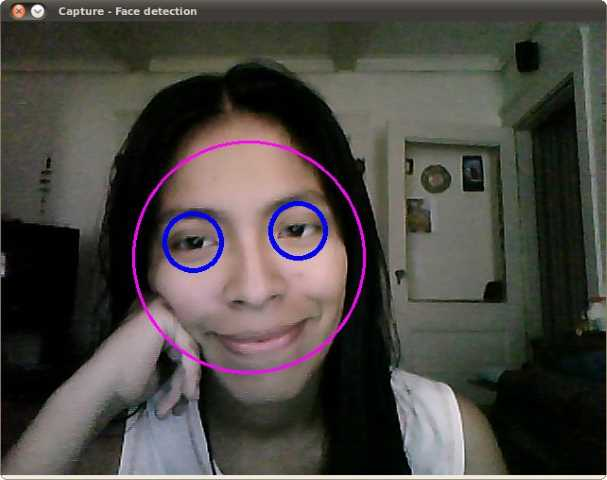
\includegraphics[width=.5\linewidth]{images/litreview/Cascade_Classifier_Tutorial_Result_Haar}
    \caption{Facial Recognition, image from \protect\footurl{https://docs.opencv.org/4.1.0/db/d28/tutorial_cascade_classifier.html}{OpenCV Cascade Classifier Tutorial}}
    \label{fig:facial}
\end{minipage}
\end{figure}

The main reasons to use OpenCV are because of its blazing speed, wide portability, and low RAM usage. It is entirely free to use, and what's more, it has frequently used and well maintained support forums, which is fantastic for when developers hit a brick wall in the applications. Further, they have annexed a set of experimental functions which extends the use cases of the library greatly.

On the other hand, reasons not to use OpenCV are that it does not provide the same ease of use when compared to other computer vision libraries such as MATLAB. In addition, the experimental modules come with the potential cost of bugs in various places, for instance, the Android pack for OpenCV with contribution modules fails to compile with their own build bots more often than it succeeds \citep{opencv-buildbot}.

\subsection{MATLAB}

Another software for computer vision is MATLAB, which is primarily designed for matrix manipulations, which makes it a good environment for data analysis and image processing. In contrast to OpenCV, MATLAB is commercial software that has more than 3 million users worldwide, and has been majorly profitable every year since its founding in 2017 \citep{matlabfacts}.

MATLAB can produce extremely stable software and functional codebase as a result of their dedicated team of professional developers, which in turn makes them popular among the masses. It can run highly parallelised code, making full use of GPUs and even clusters, which are large groups of computers that work together in a network to complete a task more efficiently. They also have the functionality to generate portable C code which can be used to develop Android and iOS applications. Further, the MATLAB GUI makes displaying output and debugging much more straightforward than its OpenCV counterpart.

Unfortunately, MATLAB requires a commercial licence to run, so to use it one must pay a fee or be fortunate enough to be under a company or campus-wide licence. Also, their libraries are well written, but not as cutting edge as OpenCV, so it fails to deliver on aspects of leading computer vision such as augmented reality.

\subsection{Summary}

After reviewing both OpenCV and MATLAB as candidates for the detection phase of this project, it is clear that OpenCV should be the method of choice, this is mostly because OpenCV is at the forefront of development for augmented reality. It is also natively portable because it is written in C++, as opposed to having to generate C code from MATLAB. The ability to parallelise MATLAB code is an excellent speedup feature; however, this project would not be able to use its full potential as the code will likely be running on a smartphone, which may be lacking in hardware.

%++++++++++++++++++++++++++++++++++++++++++++++++++++++++++++++++++++++++++++++++++
%++++++++++++++++++++++++++++++++++++++++++++++++++++++++++++++++++++++++++++++++++
%++++++++++++++++++++++++++++++++++++++++++++++++++++++++++++++++++++++++++++++++++

\section{Detection}

As mentioned previously, the detection of blocks and their poses is a vital stage of the project, and thus a key area of research. This section analyses various methods of both markerless and marker-based detection, and concludes by giving a recommendation into which method should be taken forward for design and implementation.

\subsection{Markerless Detection}\label{sec:markerless}

Markerless detection is a type of detection method used in augmented reality in which the system can detect objects in an environment without prior knowledge of that environment; this can be done by identifying features in an image and using that information to estimate the existence of a known object. A significant advantage of using markerless detection in this instance is that the \jenga{} blocks can remain unmodified and used out-of-the-box. As previously described, the best SDKs at the moment do not support detection of many objects at the same time, more specifically they would not be able to detect the poses of all 54 blocks in a tower. Therefore, it could be worth applying lower level image processing methods, such as the Hough-Lines Transform.

\subsubsection{Hough-Lines Transform}\label{subsec:hough}

The Hough-Lines transform \citep{houghpatent} is a popular feature extraction technique that can be used to identify lines that intersect many points in an image. It can also be expanded to find arbitrary objects, such as rectangles or circles. With \jenga{}, the transform can be used to detect edges of blocks which can later be used for tower reconstruction. The steps for finding lines with the hough transform are as follows:
\begin{enumerate}
    \item Load an image in grayscale
    \item Blur the image to reduce noise
    \item Apply Canny edge detection on the blurred, grayscale image
    \item Apply hough transform on the detected edges
\end{enumerate}

A simple program (\cref{code:houghpy}) was written to realize the potential of the transform with respect to block detection, the GUI for which can be seen in \cref{fig:houghscreenshot}, it shows an image for each stage of the hough transform process. Detected lines, drawn in red, can be seen traversing most edges of the tower pieces, but there are clearly edges that were missed. A serious advantage of this method is that it needs a minimal number of images, maybe even one, to get information about the tower pieces, it is therefore fast and non-intensive.

\begin{figure}[ht]
    \centering
    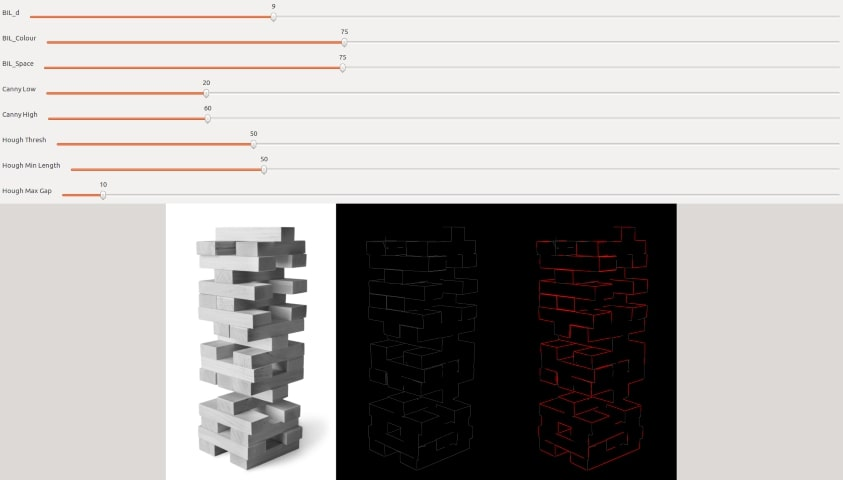
\includegraphics[width=.7\linewidth]{images/litreview/python-houghlines}
    \caption{Screenshot of hough.py program}
    \label{fig:houghscreenshot}
\end{figure}

This method would be disadvantageous to use because; it is difficult to detect every edge, meaning that a post hough-transform detection algorithm would need to be devised to find missing edges; poses would likely also be inaccurate; and the threshold values would need to be dynamic, as each environment has different lighting that would effect the methods used. Moreover, the transform has the potential to provide object tracking, but as the transform is low level, it would be hard to create a method of identifying an individual block, unlike the marker based detection methods that follow.

\subsection{Marker-Based Detection}\label{sec:markerbased}

Conversely to markerless detection, marker-based detection assumes knowledge of the environment with the use of fiducial markers. These markers are placed into the scene and are used as a point of reference to the camera, allowing for pose estimation. Two well-developed libraries to do this with are \nameandsecref{subsec:artoolkit} and \nameandsecref{subsec:aruco}, this section aims to cover the merits of both libraries and ultimately decide on which to implement in the system.

\subsubsection{ArToolKit}\label{subsec:artoolkit}

ARToolKit was one of the first libraries to make use of square markers for augmented reality applications. Its features include but are not limited to; the tracking of square markers, camera calibration, and plugins for Unity. With the kit, it is possible to get the pose of multiple markers in a single frame, which means that it would be able to detect all visible faces of blocks in a \jenga{} tower. This marker mapping feature makes it an ideal candidate for block detection.

\subsubsection{ArUco}\label{subsec:aruco}

\citet{aruco} is an alternate, newly developed library for marker-based detection. Since its inception, ArUco has been integrated with the contribution modules of OpenCV, making it a popular choice for marker detection. One of the benefits of using this library is the configurable dictionaries that aim to maximise inter-marker distance \citep{arucopaper}, hence reducing computation time when identifying markers. While the base code is written in C++, there are python and Java wrappers available, as well as cross platform support.

By itself, ArUco is unable to create a map of detected markers, however, \citet{markermapper} was created to solve this. \citet{markermapperpaper} demonstrate the effectiveness of using such a library, as it reduces pose ambiguity and can remember markers that are no longer visible to the camera. A drawback to using MarkerMapper is that if the map contains multiple components, that is if two or more maps of markers remain unconnected, the library results in a segmentation fault.

\citet{ucoslam} brings improvement to marker detection by adding functionality for simultaneous location and mapping (SLAM) of key points, and is shown to obtain better precision, robustness and speed than competing SLAM methods \citep{ucoslampaper}. This library fixes the aforementioned problem of multiple components because detected features are used to connect separate maps. It also provides an easy to understand GUI, and can be compiled for cross platform applications.

\begin{figure}[ht]
    \centering
    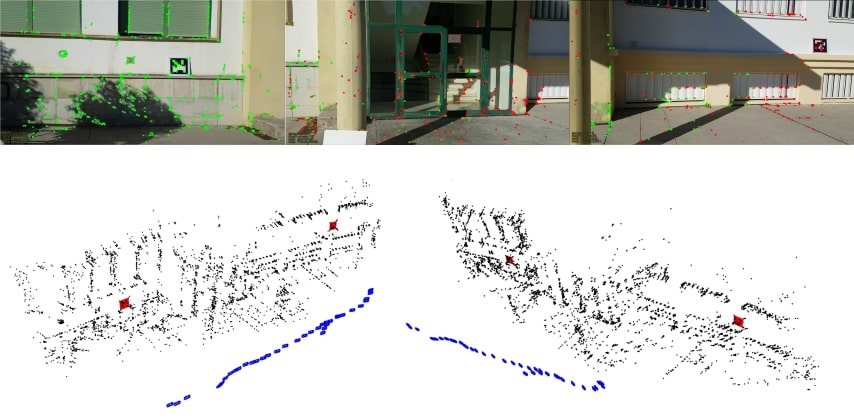
\includegraphics[width=.8\linewidth]{images/litreview/ucoslammapping}
    \caption{UcoSLAM mapping markers and key points. Image from \protect\citep{ucoslampaper}.}
    \label{fig:ucoslam}
\end{figure}

\subsection{Summary}\label{subsec:detectionsummary}

The research above shows that marker-based detection is favoured over markerless detection. Further, ARToolKit and MarkerMapper are able to produce similar results, but struggle with multiple map components. This could be an issue when detecting tower blocks because a camera may not be able to detect markers on two faces of the tower at the same time, resulting in unconnected marker poses. On the other hand, UcoSLAM would be able to detect other features of the tower, such as block corners, and use them to connect the faces of the tower. Although this means that UcoSLAM will be more compute heavy, it would be recommended to use UcoSLAM as the technology for block detection due to its obvious benefits.

%++++++++++++++++++++++++++++++++++++++++++++++++++++++++++++++++++++++
%++++++++++++++++++++++++++++++++++++++++++++++++++++++++++++++++++++++

\section{Reconstruction}\label{sec:reconstruction}

Next, to be able to analyse the structure, reconstruction must first take place, this can be done with modelling. A model is a computer-generated version of a real object which functions as if it were real. There are a multitude of methods which can be used to transform a real object into a model, these methods can be categorised in three ways:

\begin{itemize}
    \item \nameandsecref{subsec:partsbasedmodelling}, constructing a shape from a set of components
    \item \nameandsecref{subsec:voxelbasedmodelling}, constructing a shape from a set of volumetric elements
    \item \nameandsecref{subsec:viewbasedmodelling}, constructing a shape from an image or series of images
\end{itemize}

Whilst all of the methods described below are valid for constructing a model, they each have merits  and pitfalls, thus there is no 'silver bullet' approach to modelling. This section aims to provide research and critical evaluations of various methods, specifically relating to the modelling of a \jenga{} tower.
%+++++++++++++++++++++++++++++++++++++++++++++++++++++++++

\subsection{Parts-Based}\label{subsec:partsbasedmodelling}

\citet{2012probabilisticmodel} proposed a method which uses a set of shapes as training data, deconstructs them into a library of small parts, and then restructures those parts to make a set of new shapes. To do this, they used a probabilistic model to calculate which components fit together to form plausible combinations, which are defined by some optional high-level constraints. This approach proves useful in two applications; amplifying a shape database, and synthesising shapes based on high-level specifications.

An example of how this works is shown in \cref{fig:kchairs}. The model is trained on the set of chairs by taking them apart to get a set of the smallest functional components; backrest, legs, base. Next, a set of components from the training data is synthesised through the use of the probabilistic model. Finally, the components are scaled and placed together using the least-squares optimisation, thus a new shape has been synthesised.

% Chair figures
\begin{figure}[t]
\centering
\begin{subfigure}{.3\textwidth}
  \centering
  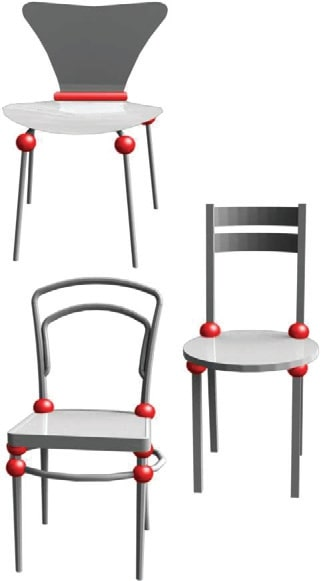
\includegraphics[width=.5\linewidth]{kalogerakis-chair-1}
  \caption{Source shapes}
  \label{fig:kchair1}
\end{subfigure}
\begin{subfigure}{.3\textwidth}
  \centering
  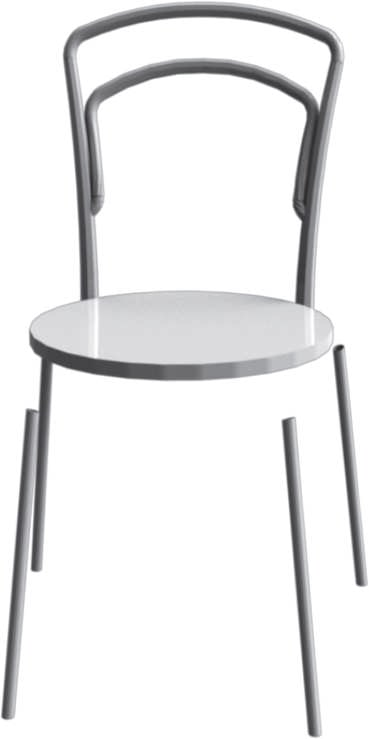
\includegraphics[width=.45\linewidth]{kalogerakis-chair-2}
  \caption{Unoptimised}
  \label{fig:kchair2}
\end{subfigure}
\begin{subfigure}{.3\textwidth}
  \centering
  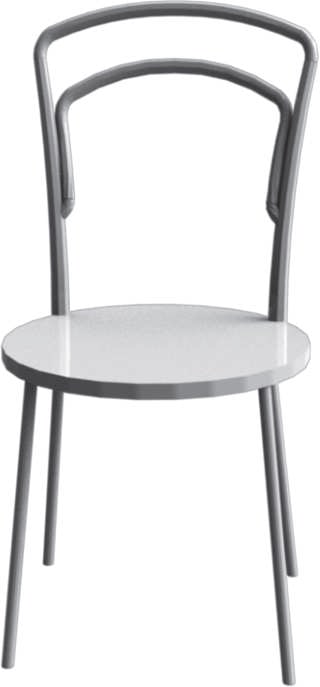
\includegraphics[width=.4\linewidth]{kalogerakis-chair-3}
  \caption{Optimised}
  \label{fig:kchair3}
\end{subfigure}
\caption{Optimising component placement. Images from \protect\citet{2012probabilisticmodel}.}
\label{fig:kchairs}
\end{figure}

A similar paper \citep{2015analysisandsynthesis} claims to have a superior approach to the synthesis of three-dimensional shapes. The method discussed in this paper is different than the one described above because it learns the geometry and deformation parameters of templates by itself, without the need to rely on pre-existing parts, which is favourable because it requires less human supervision. However, the learning is an approximation, and as such the quality of the produced shapes can be affected.

% The 3D-INN method
\begin{figure}[ht]
  \centering
  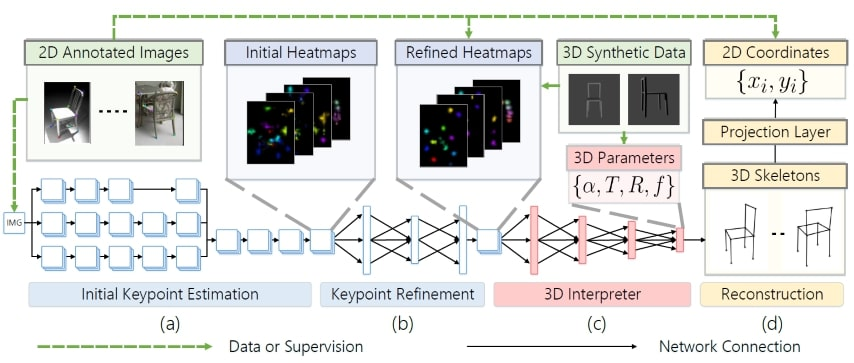
\includegraphics[width=.65\linewidth]{singleimageinterpreter}
  \caption{The 3D-INN method. Image from \protect\citet{2016singleimageinterpreter}.}
  \label{fig:3dinn}
\end{figure}

The 3D Interpreter Network method (\cref{fig:3dinn}), coined by \citet{2016singleimageinterpreter}, uses a trained framework to estimate a three-dimensional structure. The framework is trained using both synthetic 3D data and manually-annotated, real 2D images. Through the framework, they are able to extract a 3D skeleton which is treated as an abstract 3D representation. This method is part-based because the skeletons are synthesised using a predefined model for each object category, i.e. one model for all types of chair.

Finally, \citet{compoundscenesfromimages} proposed a method in which structures can be recovered from multiple silhouettes of a scene (\cref{fig:compoundscenes}). Their method works by using a library of predefined parts to find the simplest explanation of the shape of a scene. In their paper they describe that the method works for any scene, even if that scene does not contain any of the predefined parts, for example \cref{fig:eiffellego} shows a synthesised Lego construction of the Eiffel Tower. However, this method assumes that the images are taken from particular angles so that the model will not be constructed with holes when viewed from other angles.

% Lego part based modelling
\begin{figure}[ht]
  \centering
  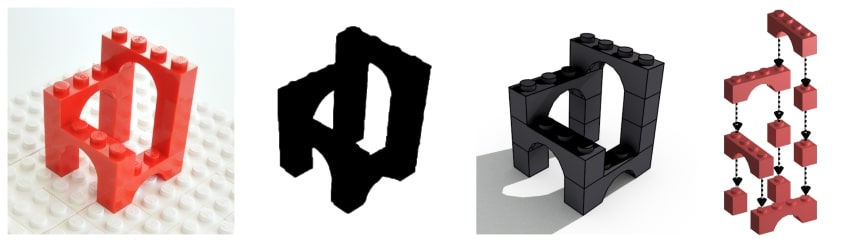
\includegraphics[width=.8\linewidth]{compound-scenes-demo}
  \caption{The part-based modelling of compound scenes from images method. Image from \protect\citet{compoundscenesfromimages}.}
  \label{fig:compoundscenes}
\end{figure}

% Lego part based modelling
\begin{figure}[th]
  \centering
  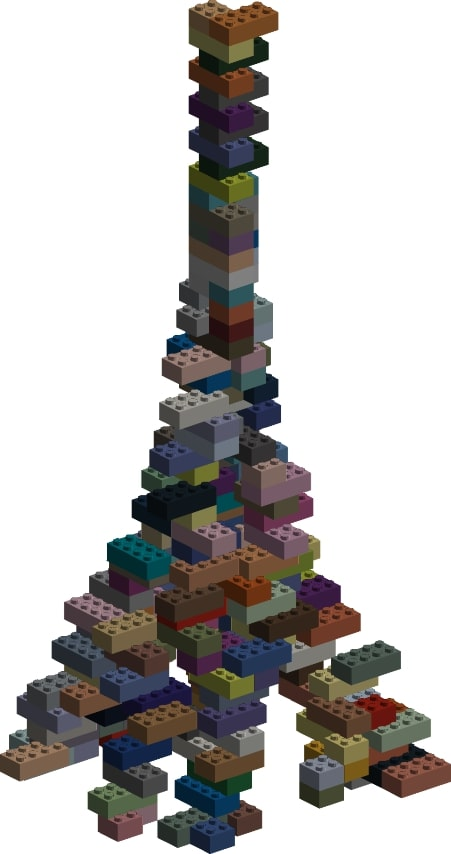
\includegraphics[height=4cm]{eiffel-tower-lego}
  \caption{Eiffel Tower constructed from Lego. Image from \protect\citet{compoundscenesfromimages}.}
  \label{fig:eiffellego}
\end{figure}

%+++++++++++++++++++++++++++++++++++++++++++++++++++++++++

\subsection{Voxel-Based}\label{subsec:voxelbasedmodelling}

A volumetric element, or voxel, represents a value in three-dimensional space akin to how a pixel represents a value in two-dimensional space. Large sets of voxels can be used to produce high quality and realistic renders of 3D shapes.

\citet{2016unsuplearning} outlined a method with which to construct a 3D shape from a 2D image using voxels. This method used end-to-end training solely from 2D images, which means they did not use any 3D annotated images, unlike a method touched on earlier \citep{2016singleimageinterpreter}. A large benefit of 2D image training in this manner is that it makes the approach entirely unsupervised. \citet{2016unsuplearning} also discuss using both volumes and meshes as elements to construct shapes, stating that volumes are flexible but introduce computational challenges, and that meshes are easier to work with, but can be restrictive in the range of shapes that they can capture.

Similarly, the 3D-GAN (3D Generative Adversarial Network) framework is learned without supervision, and has wide applications in 3D object recognition. \citet{2016problatent} state three benefits to their approach, namely the use of an adversarial criterion which allows the generator to capture object structure implicitly and thus the ability to synthesise high quality 3D shapes. Additionally they talk about the difficulty of modelling the space of 3D shapes, when compared to space of 2D objects, and how the various current approaches are promising but still produce objects with artefacts.

% The 3D-GAN method
\begin{figure}[th]
  \centering
  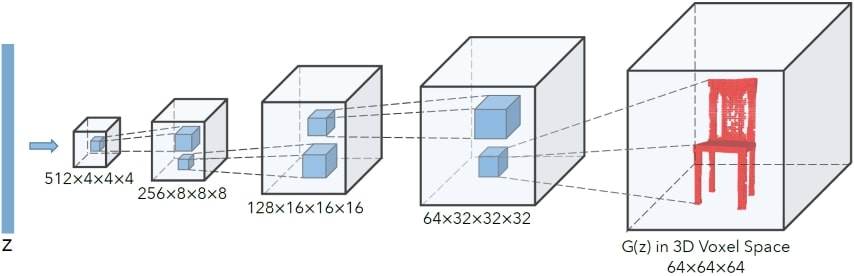
\includegraphics[width=.8\linewidth]{3D-GAN}
  \caption{The 3D-GAN method \protect\citep{2016problatent}.}
  \label{fig:3dgan}
\end{figure}

Another voxel-based modelling method, the TL-embedding network, consists of two components; an autoencoder, and a convolutional neural network (CNN). The network is multifunctional, but is focused on predicting 3D models from 2D images \citep{2016predictgenerativevector}. They specify that this approach demonstrates usefulness and versatility but the 3D representations may not incorporate the properties of the object they were synthesised from.

3D Shapenets \citep{20153dshapenets} is a model in which 3D shapes can be represented as a probability distribution of binary variables on a voxel grid. This model has the ability to recognise objects from 2.5D depth images, where a 2.5D image is effectively two-dimensional but can be perceived to have depth. \citet{20153dshapenets} learn their model using a Convolutional Deep Belief Network, though the use of a large dataset of 3D computer aided design models, and their experiments show that their representation shows significant performance improvements over previous state of the arts methods.

%+++++++++++++++++++++++++++++++++++++++++++++++++++++++++

\subsection{View-Based}\label{subsec:viewbasedmodelling}

Finally, models can be generated from a single or set of 2D images. 

\citet{2015convolutionalneuralnetworks} proposed a standard CNN architecture trained to recognise a 3D shape from a single view, with an accuracy 8\% higher than using state-of-the-art 3D shape descriptors, and their method increases in accuracy further when recognising a 3D shape from multiple views. Their method, shown in \cref{fig:multiview}, uses a view-pooling layer which is used to combine information from multiple views using their CNN architecture. What is interesting about this approach is that it can be used to recognise 3D objects even from a human sketch, as sketches can be less representative of the objects they are drawn from.

% Multiview approach
\begin{figure}[ht]
  \centering
  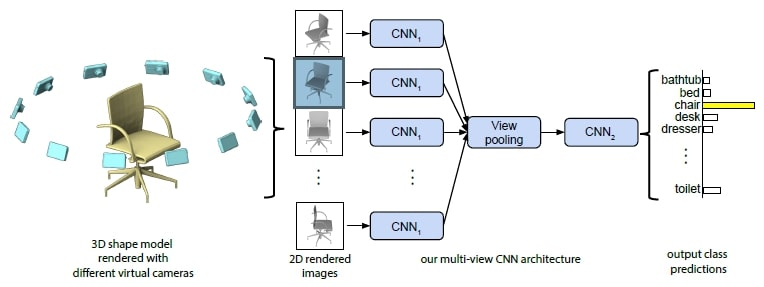
\includegraphics[width=.8\linewidth]{multiview}
  \caption{Multi-view CNN for 3D shape recognition. Image from \protect\citet{2015convolutionalneuralnetworks}.}
  \label{fig:multiview}
\end{figure}

In relation to the paper described above, \citet{2016volumetricmultiview} performed extensive experiments on the classification accuracy of state-of-the-art 3D volumetric CNN and multi-view CNN. They found that multi-view CNN far outperformed volumetric CNN, as shown in \cref{fig:volvsviewcnn}.

% Volumetric vs multiview
\begin{figure}[th]
  \centering
  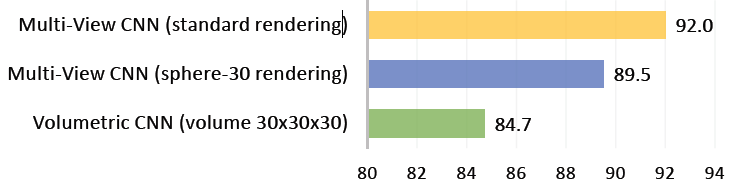
\includegraphics[width=.8\linewidth]{volumetric-vs-multiview-cnn}
  \caption{Analysis of state-of-the-art 3D Volumetric CNN versus Multi-View CNN. Image from \protect\citet{2016volumetricmultiview}.}
  \label{fig:volvsviewcnn}
\end{figure}

%++++++++++++++++++++++++++++++++++++++++++++++++++++++++++++++++++++++
%++++++++++++++++++++++++++++++++++++++++++++++++++++++++++++++++++++++

\subsection{Summary}\label{sec:categoriessummary}

The most suitable category for modelling a \jenga{} tower in this project is part-based modelling, this is mainly due to the ease of representing a tower as a combination of \jenga{} blocks. In the part-based modelling papers that were expanded in this section, most used an extensive library of 3D objects, however when modelling a \jenga{} tower only one 3D object is needed, as it can be assumed that all blocks have the same width, height and depth. Of course, the blocks may have slight variations in shape, but this can be mostly ignored for the scope of this project. A considerable benefit of using part-based modelling is that it encapsulates the reconstruction stage, and so the models created can be used directly and without further work, in the analysis stage.

In comparison, voxel-based methods can be used to synthesise high quality 3D models, but these models are likely to contain artefacts. Artefacts would be disadvantageous when creating a model of a \jenga{} tower because they would affect its structural integrity, for example a block may be generated with rough or noisy edges meaning that the blocks above it will not sit evenly on top and cause instability. So artefacts may cause an invalid representation of the real tower, making voxel-based methods less suitable to \jenga{} tower modelling.

View-based modelling has a suitability higher than that of voxel-based methods, this is because view-based methods produce models in a lower amount of time and with higher accuracy. The time it takes to model a \jenga{} tower is important because the end product needs to be able to extract structure in real-time, or close to real-time, so that the process is not painful for the user. However, view-based methods are less suitable than part-based methods because extra work needs to be done on the models after their generation to allow structural analysis to be performed.

%++++++++++++++++++++++++++++++++++++++++++++++++++++++++++++++++++++++
%++++++++++++++++++++++++++++++++++++++++++++++++++++++++++++++++++++++



%++++++++++++++++++++++++++++++++++++++++++++++++++++++++++++++++++++++++++++++++++
%++++++++++++++++++++++++++++++++++++++++++++++++++++++++++++++++++++++++++++++++++
%++++++++++++++++++++++++++++++++++++++++++++++++++++++++++++++++++++++++++++++++++

\section{Analysis}\label{sec:structuralanalysis}

The main objective in \jenga{} is to remove a block from the tower and place it on top, in such a way that the tower remains structurally intact. Choosing which block to remove is a difficult task, as the analysis relies heavily on the physics of structural engineering. This section will provide a background in a few types of structural analysis, namely \nameandsecref{subsec:rulebased}, \nameandsecref{subsec:physicssimulation}, and \nameandsecref{subsec:machinelearning}, it will then give a summary of what was researched and identify some key points for consideration later on in the project.

%++++++++++++++++++++++++++++++++++++++++++++++++++++++++++++++++++++++
%++++++++++++++++++++++++++++++++++++++++++++++++++++++++++++++++++++++

\subsection{Rule-Based Analysis}\label{subsec:rulebased}

\citet{jengaanalysis} researched into the translations and rotations that can be performed on \jenga{} blocks in a tower to find out which moves are safe from disturbing other blocks. He concluded that the movement that resulted in the least disturbance to the tower, for a centre block, was one which included no rotation, and only translation in a single direction; perpendicular to the face of the tower that the block is being removed from.

In his paper, he also mentions the most significant factor that complicates the game is the variability of the game pieces, a fact confirmed by \jenga{}'s creator \citep{jengacreator}, this is because smaller blocks can become free-floating, and larger blocks can become load bearing. When rebuilding the tower in a virtual space, it would be difficult to counteract this problem unless the blocks had their dimensions measured individually, which is a time sink and reduces the usability of the system.

\begin{figure}[ht]
    \centering
    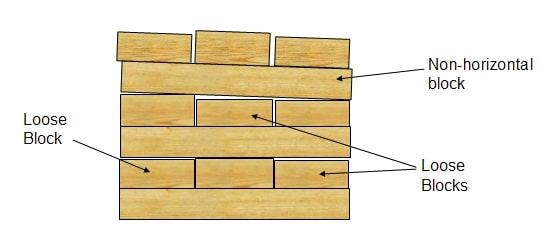
\includegraphics[width=.8\linewidth]{images/litreview/jenga-different-sizes}
    \caption{A side view of a \jenga{} tower \protect\citep{south2003real}}
    \label{fig:jengasizes}
\end{figure}

In another light, \citet{jengarobot} created a robot capable of playing \jenga{} for a tower of up to 9 layers, although the robot wasn't able to place the pieces back on top of the tower. His paper was full of useful information about the block extraction process, including the differences between side and centre blocks. It was established that the centre pieces were easier to remove, but subsequent moves on that layer would result in collapse, in contrast, both edge pieces could be removed on one level with minimal affect on the tower stability.

In summary, it is plausible to have a set of rules accurate enough for rule-based analysis, yet it may not be the most effective way to analyse the tower. This analysis method only provides simple rules, and is missing more advanced constraints such as friction and weight distribution.

%++++++++++++++++++++++++++++++++++++++++++++++++++++++++++++++++++++++
%++++++++++++++++++++++++++++++++++++++++++++++++++++++++++++++++++++++

\subsection{Physics Simulation}\label{subsec:physicssimulation}

This section will review some of the many \jenga{} simulators already exist, and discuss their uses in this project.

\subsubsection{\protect\possessivecite{github-Physijs} Jenga Physijs}

A fantastic simulator using the Physijs implementation of ammo.js, a Bullet physics engine. On opening the simulator, the tower visibly sways a small amount, indicating that the pieces all have pre-allocated positions in the world, and when gravity acts on the tower, it moves slightly until it reaches equilibrium. On moving the blocks, the inter-block contact feels slippery, as if the friction was not quite calibrated to real-world \jenga{} blocks. The physics of the tower seems to accurately represent what would happen with a real tower in the same state.

There was however a major problem found during testing; occasionally when moving a piece, it would shoot off at high speed, which is unrealistic. It is possible that the simulator misinterpreting mouse events could cause this, but could also be due to the weight of the tower forcing the block out, either way this kind of bug is game-breaking.

The source code is available on GitHub so it would be possible to fork the project for use in this paper, but the game-breaking bug would have to be addressed, and functions added for importing a tower state.

\begin{figure}[ht]
\begin{minipage}{0.45\textwidth}
    \centering
    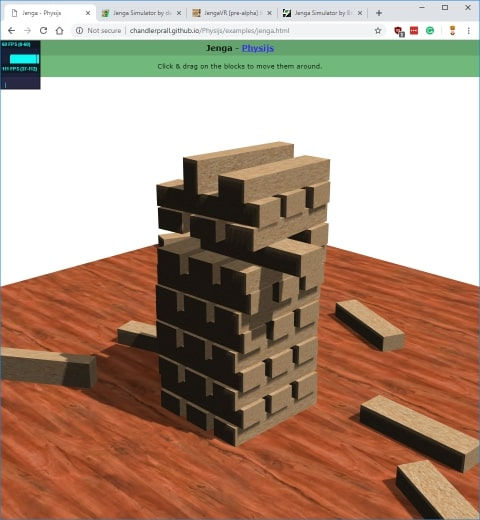
\includegraphics[width=.8\linewidth]{images/litreview/jenga-2}
    \caption{An instance of Jenga Physijs \protect\citep{github-Physijs}}
    \label{fig:simulator1}
\end{minipage}\hfill
\begin{minipage}{0.45\textwidth}
    \centering
    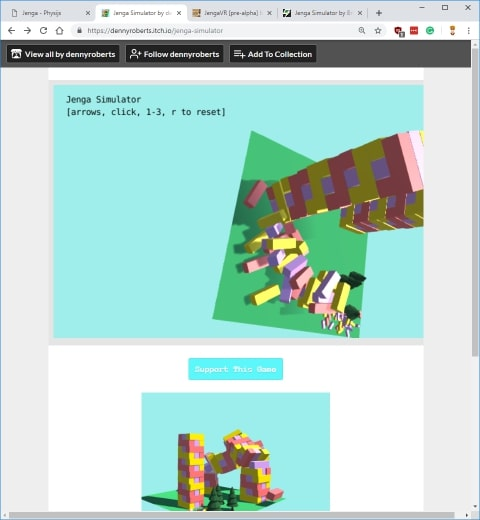
\includegraphics[width=.8\linewidth]{images/litreview/jenga-1}
    \caption{An instance of Jenga-Simulator \protect\citep{itchjenagasimdennisroberts}}
    \label{fig:simulator2}
\end{minipage}
\end{figure}

\subsubsection{\protect\possessivecite{itchjenagasimdennisroberts} Jenga-Simulator}

This simulator is built in Unity for use on the web; it has a distinctive multicoloured theme which makes it easy to distinguish between the tower pieces. On startup, the game drops a set of blocks from the sky onto a small platform, where they settle to form towers, immediately it can be seen that this sequence would fail to work with an imported tower of any other state than the starting state.

It also works by clicking, instead of dragging, which makes for a rather odd experience. As a result of only allowing clicks, movements are restricted to translations, which meant that removing by rotation was out of the question. Another aspect that stood out was that the whole scene moved when clicking, and therefore the whole tower was affected regardless of whether a block could be removed successfully.

In terms of friction though, this simulator stood above \possessivecite{github-Physijs} because it did not feel slippery, but more like real movements of \jenga{} blocks.

\subsubsection{\protect\possessivecite{itchjengasimben} JengaVR}

JengaVR is only available in virtual reality, and due to limited access to VR headsets, first-hand testing could not be done. Nonetheless, there are a couple of videos on the web in which this game was played, and as such this review is completed from watching the game second-hand.

It was nice to see that the in-game blocks had the same texture as real \jenga{} blocks, as it allowed for a more immersive experience. Picking out pieces of the tower looked intuitive, as the player can use hand-held controllers similar to how they would play outside of the virtual world.

Further, the tower seemed shaky at times and swayed at others. At one point, a block was edging inside of another, meaning that the collision detection was not as accurate as it should be. Also, the tower looked like it should have fallen over in a couple of states, but this was maybe prevented by a higher amount of friction in the game engine.

\begin{figure}[ht]
    \begin{minipage}{0.45\textwidth}
        \centering
        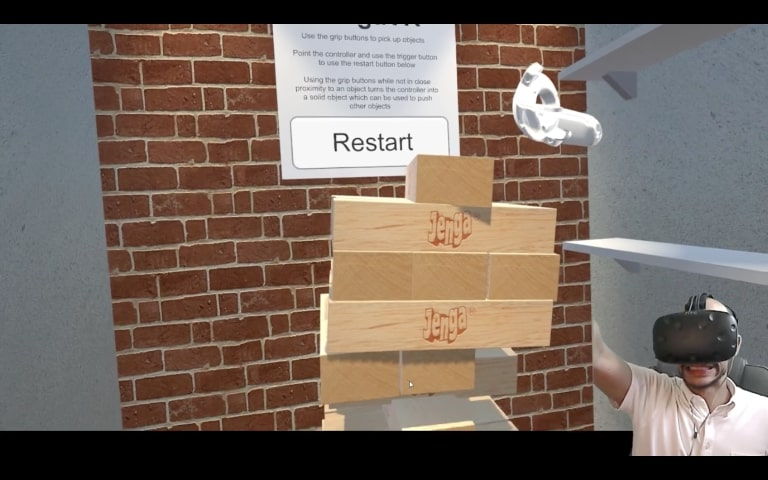
\includegraphics[width=.9\linewidth]{images/litreview/jenga-3}
        \caption{Screencap from the JengaVR trailer \protect\citep{github-Physijs}}
        \label{fig:simulator3}
    \end{minipage}\hfill
    \begin{minipage}{0.45\textwidth}
        \centering
        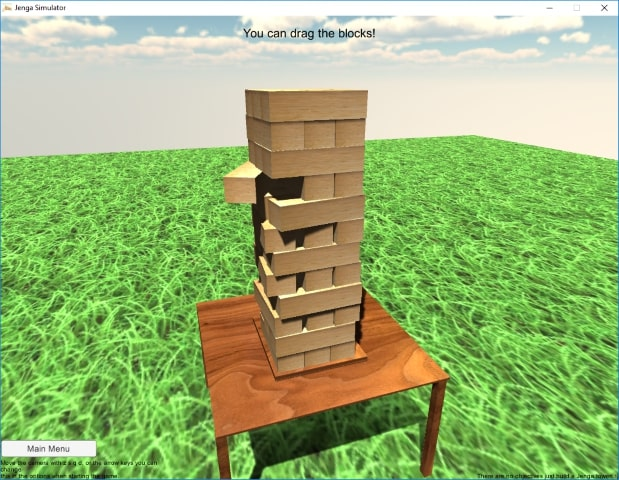
\includegraphics[width=.9\linewidth]{images/litreview/jenga-4}
        \caption{An instance of Jenga-Simulator \protect\citep{gamejoltjengasim}}
        \label{fig:simulator4}
    \end{minipage}
\end{figure}

\subsubsection{\protect\possessivecite{gamejoltjengasim} Jenga-Simulator}

In this Windows based Jenga-Simulator, a \jenga{} tower sits on top of a table in a semi-realistic world, for the user to play with. Blocks can be dragged with the mouse, and the camera moves on a plane on one side of the tower, if any of the blocks fall, the game restarts.

Removing pieces from the tower in this game proved more difficult than any of the other simulators, perhaps due to the high amount of friction, which may have been avoided by creating slight variations in the block dimensions, as it allows for free-standing pieces.

This game was the most fun to play, but it did not feel realistic, which was partly due to the blocks not being of the standard \jenga{} dimensions, and also because of the difficulty in removing the pieces.

\subsubsection{Summary}

All of the above were made to be played as games, not realistic simulators, so during development there was bound to be decisions which opted for enjoyability over realism. One of these decisions was to create blocks that did not accurately represent the size of \jenga{} blocks. Despite this, there is still a lot that can be learned from these projects.

Firstly, creating blocks of randomly varying sizes would fix some of the issues observed, but the same could not be said for the system proposed in this document.  If the tower were to be built with varying sizes, they would have to be the real sizes of the blocks, not random; otherwise the simulation would not accurately represent the real tower.

A common issue was that the friction was either too high, causing difficulty in removal, or too low, causing a slippery feel to the game. It would be beneficial to test out several settings of friction during the development of this project, to ensure realism is achieved.

%++++++++++++++++++++++++++++++++++++++++++++++++++++++++++++++++++++++
%++++++++++++++++++++++++++++++++++++++++++++++++++++++++++++++++++++++

\subsection{Machine Learning}\label{subsec:machinelearning}

Machine learning, a term coined by \citet{machinelearning}, is the study of computer algorithms which rely on patterns and inference to perform specific tasks. The taxonomy of these algorithms include; supervised learning, where the algorithm learns with labels given by human input, unsupervised learning, where the algorithm learns without human input, and reinforcement learning, where the algorithm learns a policy of how to act given an observation of the world, i.e. learn from its mistakes \citep{machinelearningtypes}.

In essence, machine learning is used for tasks that are too complex for developers to code a solution for themselves, and is therefore useful in many areas; applications range from autonomous helicopter aerobatics \citet{autonomoushelicopter}, to the early detection of heart failure \citep{machinelearningheart}. There are numerous factors involved with the physics of a \jenga{} tower, making it difficult to accurately assess, this section discusses whether it would be appropriate to involve machine learning to aid in the analysis.

\subsubsection{Supervised}

Supervised learning is maybe the most popular paradigm for machine learning; it is synonymous with giving an algorithm labelled data which are then used to predict the classification of unseen data. This project could make use of supervised learning techniques by generating a set of training data which would include a great many variations of tower states, and then labelling each state with either stable, or unstable. During system runtime, if the algorithm comes across a tower state that is not included in the training data, it would then be able to give a prediction on the classification of tower state.

Although popular, this type of machine learning would require a lot of time spent training, as the human trainer would need to manually classify each state, and so would not be an ideal choice of method for this project.

\begin{figure}[ht]
\begin{minipage}{\textwidth}
    \centering
    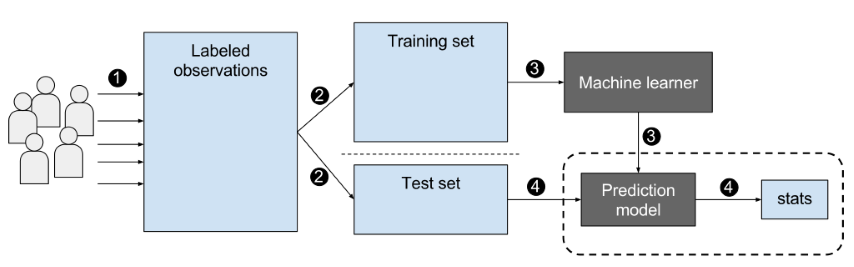
\includegraphics[width=.8\linewidth]{images/litreview/Supervised_machine_learning_in_a_nutshell}
    \caption{Supervised learning from  \protect\footurl{https://blogs.nvidia.com/blog/2018/08/02/supervised-unsupervised-learning/}{Nvidia Blogs}}
    \label{fig:supervisedlearning}
\end{minipage}
\end{figure}

\subsubsection{Unsupervised}

On the other hand, unsupervised learning is a data-driven approach that does not require labelling; it is instead fed data and tries to discover the underlying structure of that data. As a result of the learning being unsupervised, there is no way to determine what the outcomes would be, nor how accurate they are, and as such, this approach is not well suited to classification problems. 

In the case of this project, the data would again be a set of many variations of tower states, but the results could be wildly different the supervised approach. It would be interesting to see what these would be, but probably falls out of the scope of this project.

\subsubsection{Reinforcement}

Finally, reinforcement learning is an machine learning approach akin to Pavlov's dog \citep{pavlovdog}, in which the behaviour conditioning of dogs were recorded in response to varying stimuli. With respect to machine learning, this technique allows an algorithm to learn from mistakes, by providing it with positive and negative signals after performing a task.

\begin{figure}[ht]
    \centering
    \begin{tikzcd}
        Perception \ar[r] & Action \ar[r] & Reward \ar[ll,bend left,"repeat"]
    \end{tikzcd}
    \caption{Reinforcement learning pipeline}
\end{figure}

This approach would encompass giving the algorithm full reign of a \jenga{} simulator, meaning it would have the ability to move blocks, just like a human would in the real world. First, the algorithm would choose a block, and attempt to remove it, if the removal causes the tower to fall over then it would record the result as a negative stimulus, otherwise a positive result would be recorded. Then, the tower would be rebuilt and the process would repeat itself many times over, with the algorithm learning with each iteration.

\subsubsection{Summary}

In summary, given a trained algorithm, the system would be able to analyse the structural integrity of a \jenga{} tower, and give the user a prediction of the removal feasibility of each block. The preferred method described above is reinforcement learning, this is because of it's ability to learn from its mistakes, and because it is a more autonomous technique than supervised learning, which would require lots of human input. In contrast, unsupervised learning would not be ideal for this project as the results would be unpredictable.

%++++++++++++++++++++++++++++++++++++++++++++++++++++++++++++++++++++++++++++++++++
%++++++++++++++++++++++++++++++++++++++++++++++++++++++++++++++++++++++++++++++++++
%++++++++++++++++++++++++++++++++++++++++++++++++++++++++++++++++++++++++++++++++++

\section{Visualisation}

The last area to be researched for this project is the presentation stage. The topics covered in this background study comprises of visual display techniques, including augmented reality, and graphical user interfaces (GUIs).

%++++++++++++++++++++++++++++++++++++++++++++++++++++++++++++++++++++++
%++++++++++++++++++++++++++++++++++++++++++++++++++++++++++++++++++++++

\subsection{Head-Worn Displays}

Head-worn displays boast a more immersive experience than AR on smartphones, yet they can be considerably more expensive. Currently, there are a wide variety of head-worn displays on the market, some of which are reviewed below with relation to this project.

\subsubsection{Microsoft HoloLens 2}
The HoloLens 2 \citep{hololens2} is the latest in the line of HoloLens headsets, with improvements over its predecessors such as a wider field of view, eye tracking sensors, and being lighter in weight. Although, with a price tag of \$3,500, this device is not aimed towards the general public, but mostly at businesses that could see improvements through the use of AR, such as factory workers. A consequence of the cost to purchase the HoloLens is that it would be infeasible to use in an undergraduate project.

\subsubsection{North Focals}
More realistically priced, the \citet{northfocals} are a pair of AR glasses that cost around \$599. They look like standard, non-technological glasses, but have much functionality built in, like text messages, music and maps. While aesthetically pleasing and custom built, these glasses seem to be great for the everyday consumer, when it comes to augmented reality for gaming, they fail to deliver, due to their low specification hardware.

\subsubsection{Intel Vaunt}
HoloLens and North Focals both use a screen display method, Intel's Vaunt breaks this pattern by using laser projection; the glasses work by reflecting a laser beam into the eyeball, and onto the retina. The laser used is of class one, which means it is very low powered, and will not cause harm to the eye. Unfortunately, the Vaunt is officially no longer being developed \citep{intelvaunt}, so it would not be possible to use it in this project.

\subsubsection{Magic Leap One}
The \href{https://www.magicleap.com/magic-leap-one}{Magic Leap} (\citeyear{magicleap}) is also separate from on-screen AR display, as it projects a digital light field into the user's eye \citep{redditmagicleap}, which is apparently the only safe way forward for authentic replication of visual reality. It requires the user to carry around a small Lightpack which performs all of the computations for displaying AR with the goggles, while retaining its mobility. It also has a controller, which allows it to be used for games, so in that respect, it would be suitable for use in this project. But as an emerging technology, the Magic Leap One is not yet available to consumers, but people in a few United States cities do have access to the device in a development capacity.

\begin{figure}[ht]
\begin{minipage}{\textwidth}
\begin{minipage}{0.5\textwidth}
    \centering
    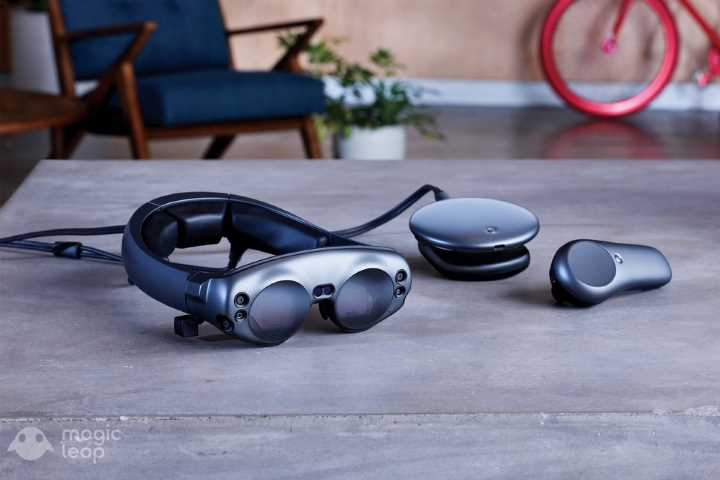
\includegraphics[width=0.9\textwidth]{images/litreview/magicleap}
    \label{fig:magicleap}
\end{minipage}\hfill
\begin{minipage}{0.5\textwidth}
    \centering
    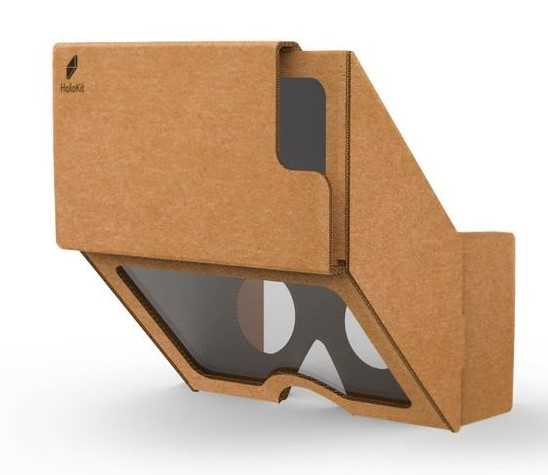
\includegraphics[width=0.7\textwidth]{images/litreview/holokit}
    \label{fig:holokit}
\end{minipage}
\caption{The \protect\footurl{https://www.magicleap.com/magic-leap-one}{Magic Leap One} (left) and the \protect\footurl{https://holokit.io}{HoloKit} (right)}
\end{minipage}
\end{figure}


\subsubsection{Lenovo Mirage}
Down in the low end of AR headsets sits the \href{https://www.lenovo.com/gb/en/jedichallenges/}{Lenovo Mirage} (\citeyear{jedi}), at just \pounds89.99, providing an experience like no other around today. This device is built solely for AR gaming, specifically for Star Wars, a popular film and tv franchise; it offers lightsaber duels, ship battles, and other strategic games, all played in augmented reality. Also, the headset requires a smartphone, which is used as a display device; meaning it would be useful in this project as any smartphone app can be used.

\subsubsection{HoloKit}
Related to the Lenovo Mirage, the \href{https://holokit.io}{HoloKit} (\citeyear{holokit}) requires a smartphone to function. It is made from cardboard and works by having the phone reflect its display onto a mirror next to the user's eyes. Moreover, it is maybe the cheapest AR headset available today, owing to its minimalist design. The HoloKit software development kit (SDK) is available on GitHub and uses the Unity game engine to create applications.

\subsubsection{Summary}
It is exciting to use augmented head-worn displays because they use cutting edge technologies, meaning that many of the experiences they offer have never been seen before.  However, this also brings drawbacks, namely the high prices and low availability. A common theme among the above devices is the inability to provide gaming in the experience; this is because some of the glasses are not designed for such functions. They also need to have high mobility, as they are expected to be used in a diversity of environments, and need to be as efficient as possible, leading to lower power consumption and consequently lower battery sizes. 

The most appropriate displays identified are the Lenovo Mirage and HoloKit because of their incorporation of smartphones, meaning they can display any mobile application, at a low cost. Although, if considering this route it would be less expensive to not use a head-worn display at all, with the downside of having to hold the phone with hands.

All things considered, head-worn displays are not yet quite as developed, economical, or featureful as would be needed for a project of this description, and so it would be recommended not to use headsets.

%+++++++++++++++++++++++++++++++++++++++++++++++++++++++++

\subsection{Software Development Kits}

In order to develop applications in augmented reality, software development kits (SDKs) must be used. AR SDKs are bundles of useful functions that allow developers to interact with the environment through various computer vision techniques, which saves time during application development because it prevents reinventing the wheel. This section shows the research completed into four of the significant AR SDKs prevalent today that work with modern smartphones; Vuforia, ARKit, ARCore, and ARToolkit.

\subsubsection{Vuforia}
\href{https://www.ptc.com/en/products/augmented-reality}{Vuforia} (\citeyear{vuforia}) is an SDK which provides recognition for objects, text and environment. It is marketed mainly for industrial use, including solutions for manufacturing, reducing service costs, and sales. Also, it prides itself with a powerful object scanner, which allows the user to scan and create real object targets for rigid objects that can fit on a tabletop.

\begin{figure}[ht]
\begin{minipage}{\textwidth}
    \centering
    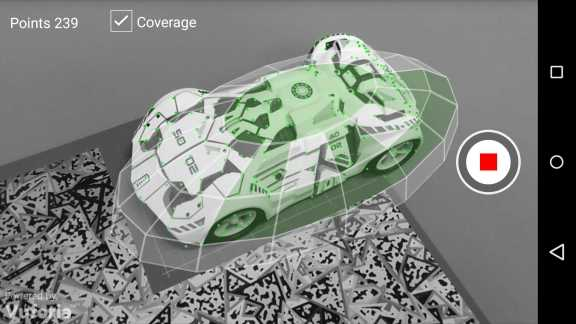
\includegraphics[width=0.6\textwidth]{images/litreview/vuforiaobject}
    \caption{Object scanning in Vuforia, image from \protect\footurl{https://library.vuforia.com/articles/Training/Vuforia-Object-Scanner-Users-Guide}{Vuforia Users Guide}}
    \label{fig:vuforia}
\end{minipage}
\end{figure}

This scanner could be used to create a virtual \jenga{} block object, with high precision, and later used for augmented display. Alas, the engine only supports tracking of up to two objects at a time, rendering this solution unworthy, at least while the object tracking limit remains this low.

\subsubsection{ARKit}
Apple Inc. purchased the \citeauthor{arkit} in 2015, and have continued development since then, so far providing features such like; the TrueDepth camera system, which combines several sensors to get an accurate understanding of depth in images; visual inertial odometry, where the pose of a camera can be estimated using images of its environment; ambient lighting estimation, which it uses to update the colours of virtual objects based on its surrounding light.

ARKit, as with most Apple products, is contained within the Apple ecosystem, which means that the SDK is only available on a few select smartphones produced by the company. As a direct result from this, ARKit was not able to be used in this project on account of limited resources.

\subsubsection{ARCore}\label{sec:arcore}
Similar to ARKit is Google's \citet{arcore}, which shares many of its features, and adds motion tracking and more advanced environmental understanding, allowing for augmented objects to be seemingly connected to real-world objects, rather than just superimposed. In contrast to ARKit, ARCore is available on a plethora of devices, including some on iOS.

Currently, the SDK can track objects, but this is implemented to estimate the camera pose, so it would be ineffective for predicting individual block poses. However, a solution in which the tower is tracked as a single rigid object may be viable with this technology.

\begin{figure}[ht]
\begin{minipage}{\textwidth}
    \centering
    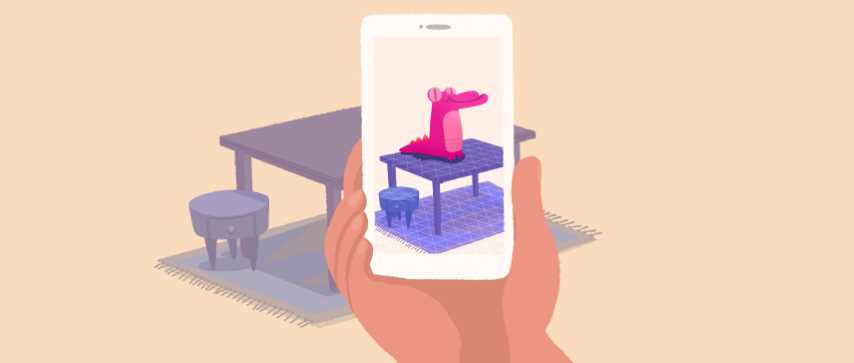
\includegraphics[width=0.8\textwidth]{images/litreview/EnvUnderstanding}
    \caption{Environmental understanding in ARCore, from \protect\footurl{https://developers.google.com/ar/discover/concepts}{Google Discover Concepts}}
    \label{fig:arcoreenv}
\end{minipage}
\end{figure}

\subsubsection{ARToolKit}
\citet{artoolkitandroid} reviewed the development process of creating an augmented reality application for Android devices using the \citet{artoolkit} SDK, an open source library that implements the logic necessary for AR applications. In the report she says that the SDK works with ordinary phones and webcams, which is unlike the kits reviewed above, as they all require reasonably well-powered smartphones. A key feature in ARToolKit is marker tracking and pose estimation, this allows the developer to track multiple objects at a time, provided they have markers attached.

\subsubsection{Summary}
The software development kits described above are all at the forefront of AR technology today, and so represent the best functionality that AR has to offer. After review, it is clear that tracking objects, such as \jenga{} blocks, would be difficult, unless marker based AR is used. Otherwise, it may prove worthwhile to track the tower as a single structure, and augment information directly onto that, but this has its own drawbacks, for instance the pieces would not be able to be tracked when being removed from the structure. The next sections delve more into this discussion by comparing markerless and marker based AR.

\subsection{Interfacing}

Paired with an augmented display, a graphical user interface (GUI) is key to providing the user with a pleasant experience. Much research has been completed in this topic, from this research, the section below gives some insight into what it takes to design an efficient and user-friendly interface.

\possessivecite{guirooms} paper on designing user interfaces is an example of early work in the field; it focuses on reducing space contention in a window-based GUI by using a window management concept called Rooms. Although this paper was written a couple of decades before the rise of smartphones and AR, there are still some relevant points to be considered. One of which is to avoid the ``electronic messy-desk problem'', where too many items are displayed on a screen, leading to a reduction in workspace efficiency and performance.

More recently, \citet{guienergyefficiency} showed that significant improvements to GUIs can be made by employing energy efficient design techniques. A survey they conducted found several intuitions into GUI use, such as; users find small buttons annoying, users prefer interfaces that are easy to learn and allow them to work faster over good-looking interfaces, as well as liking features which display progress is being made, such like an hourglass.

Furthermore, usability studies show great promise in the design of user-friendly mobile interfaces. \possessivecite{guiusabilityreview} review into the area concluded that some of the main qualities in the design of these interfaces are limited screen size, lack of physical response and high demand for visual attention. It is, therefore, necessary to take into account these areas when designing the interface for the proposed solution in this document.

A current interface can be seen when using the IMDb smartphone app (\cref{fig:imdb}), which uses many features common to applications today. The app keeps the amount of displayed text minimal, so as to rapidly identify areas of importance to the user, such as headings. It also uses large images, this is because images are more interesting than text and serve to capture the users attention. In addition, IMDb has uses a scrolling interface which allows the user to display more content when they have finished consuming the current content, this is useful when an app has more information than it can comfortably fit on one screen. Another point of reference is the tab bar layout at the top of the app, which makes it clear which page the user is currently viewing, and allows the user to switch between pages with ease.

\begin{figure}[ht]
\begin{minipage}{\textwidth}
    \centering
    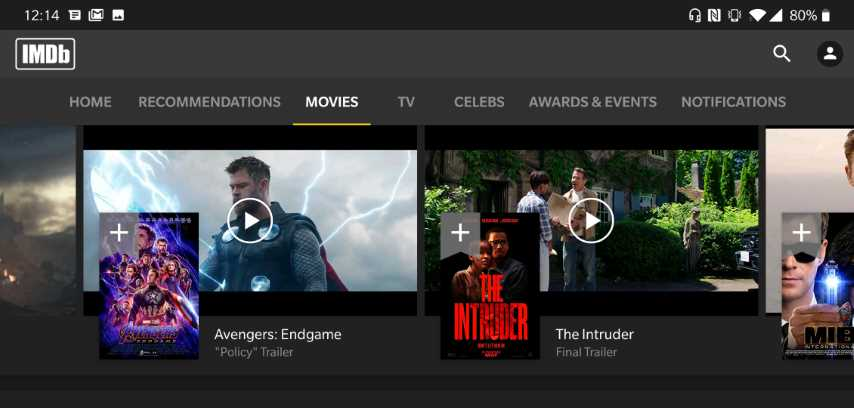
\includegraphics[width=\textwidth]{images/litreview/imdb-screenshot}
    \caption{A modern smartphone interface, from the \protect\footurl{https://play.google.com/store/apps/details?id=com.imdb.mobile&hl=en_GB}{IMDb Android Application}}
    \label{fig:imdb}
\end{minipage}
\end{figure}

%++++++++++++++++++++++++++++++++++++++++++++++++++++++++++++++++++++++++++++++++++
%++++++++++++++++++++++++++++++++++++++++++++++++++++++++++++++++++++++++++++++++++
%++++++++++++++++++++++++++++++++++++++++++++++++++++++++++++++++++++++++++++++++++

\subsubsection{}

This chapter has researched and discussed various literature and technology surrounding the project scope. Findings from this background study will influence the decisions made later on in the project, including being the main source for the capture of requirements, which will follow.

%++++++++++++++++++++++++++++++++++++++++++++++++++++++++++++++++++++++++++++++++++
%++++++++++++++++++++++++++++++++++++++++++++++++++++++++++++++++++++++++++++++++++
%++++++++++++++++++++++++++++++++++++++++++++++++++++++++++++++++++++++++++++++++++

%---=---==---===---====---=====---======---=====---====---===---==---=---%
%-         REQUIREMENTS ANALYSIS AND REQUIREMENTS SPECIFICATION         -%
%---=---==---===---====---=====---======---=====---====---===---==---=---%

\chapter{Requirements}\label{chap:requirements}

This chapter focuses on project requirements. It begins with an explanation of the process of requirements \nameandsecref{sec:requirementscapture} and analysis, continues with a discussion of crucial \nameandsecref{sec:requirements} and areas of particular challenge, and then ends with addressing, with prudence, the issue of project \nameandsecref{sec:scope}.

\section{Capture} \label{sec:requirementscapture}

Requirements are an essential aspect of any project, as they formulate the purpose of the software, and set clear goals. Without requirements, developers may lose sight of what needs completing, and so may fail to deliver as expected; it would also cause problems in testing, as testers would be unable to refer to how an application should function. A keen effort was made to develop specific requirements, with low ambiguity, and written concisely.

In this project, the requirements were captured from the \nameandsecref{chap:background}, through research and technology review. Relevant academic papers were evaluated to ascertain what is possible to develop using current state-of-the-art methods, and these are reflected on in the requirements. Also, technology was reviewed to determine what had gone well, not so well, and what to avoid doing from previous projects.

Another method used for requirements capture was the short coding exercise in \cref{subsec:hough}, which was key to the capture process. Short coding can quickly validate a method before allotting it a more substantial amount of time, in this case, time was saved by determining that using markerless detection methods; specifically, the Hough-Lines transform, was infeasible.

\section{Requirements} \label{sec:requirements}

Using the techniques discussed previously in \cref{sec:requirementscapture}, this section aims to formulate requirements in response to the problems identified in \cref{sec:challenges}. It opens a discussion into the critical requirements in each stage of the system, explains why they were chosen and focuses on areas of particular challenge, difficulty or conflict. The full breakdown of requirements can be found in \cref{app:requirements}.

\subsection{\detection}



As was summarised in \cref{subsec:detectionsummary}, the system should use marker-based detection methods because of its clear advantages over markerless detection. Namely, it allows for an immediate understanding of object poses without the need for further analysis. Another reason to use marker based detection is that if a marker is detected, then it is known that a block exists at that location, meaning that it implicitly meets \cref{req:blocknonblock,req:tower}, which would otherwise require explicit solving.

Moreover, UcoSLAM is a library well fit for this project, due to its ability to map the locations of both markers and key points, thus gaining a deeper understanding of the environment, and so it should be adopted as the method of choice.

\subsubsection{Pose Estimation}\label{subsec:poseestimation}

There are a few options to consider for how to employ marker-based detection with a \jenga{} tower, in particular, answering the question of which block faces should markers be affixed. Firstly, affixing markers to every face would be a viable solution, as it means every block face can be identified and have its pose estimated; however, this solution involves a high setup time cost, and it also requires a larger dictionary of markers. Using a larger dictionary is disadvantageous because it means that the detection algorithm needs to search for more markers, thus increasing detection time, and also resulting in a higher chance for errors, i.e. false positives \citep{ucoslampaper}.

The opposite of the above solution is only to use one marker per block, which is better because it has less setup time, and requires a smaller dictionary size. If a single marker is attached to an end face of a block, then after estimating its pose, the full block pose can be estimated by using known dimensions, which in the official game are 15mm x 25mm x 75mm. On first look, this solution seems like it would be successful, although the faces are small, and markers will have to be even smaller, as there needs to be a relatively small amount of whitespace around each marker so that the detection algorithm does not confuse multiple markers as being part of one. Also, small markers are subject to pose ambiguity, as shown in \cref{fig:poseambiguity}, so although a marker pose estimations may be incorrect.

\begin{figure}[ht]
\begin{minipage}{\textwidth}
    \centering
    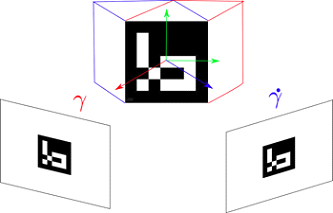
\includegraphics{images/requirements/ambiguity_problem.png}
    \caption{The ambiguity problem, image from the \protect\footurl{https://docs.google.com/document/d/1QU9KoBtjSM2kF6ITOjQ76xqL7H0TEtXriJX5kwi9Kgc}{ArUco Documentation}}
    \label{fig:poseambiguity}
\end{minipage}
\end{figure}

The ArUco library tries to solve the ambiguity itself, by using various error correction methods, but there is a way to can solve the ambiguity problem with \jenga{} pieces; that is affixing a marker to both end faces of each block. This eliminates the problem by estimating the position and orientation of both markers for a tower piece, and then reconstructing the piece to be between the two markers. In fact, this method means that the pose of each marker can be discarded, as only their relative locations are required for reconstruction.

\subsubsection{Camera}

A problem that comes with marker-based detection is camera distortion, which is common with modern cameras. Distortion is a problem because it means that two separate cameras could look at the same environment and come to a different understanding. As this project plans to solve the block removal problem in a real-world environment, as opposed to a lab-style fixed-camera environment as in previous solutions, this solution must account for camera-specific distortion, which brings about the need for \cref{req:camera}.

\begin{figure}[ht]
\begin{minipage}{\textwidth}
    \centering
    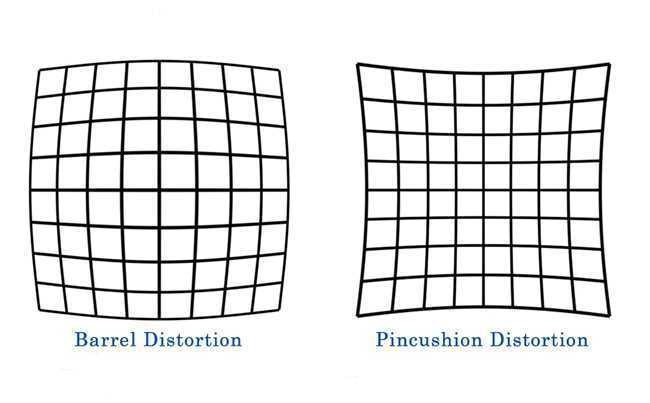
\includegraphics[width=.6\textwidth]{images/requirements/camera-distortion.jpg}
    \caption{Camera distortion, image from \protect\footurl{https://clickitupanotch.com/lens-distortion/}{Click it up a Notch}}
    \label{fig:cameradistortion}
\end{minipage}
\end{figure}

Another critical requirement is that the detection stage must be able to send the information it acquires about the block poses to the analysis stage, this is because a working system must have communication between its components; otherwise, it is not a single system, but a sum of separate components. Also, the stages may be written in different languages, so communication should be language independent. The requirements for the analysis stage are described next.

\subsection{\analysis}

\cref{sec:categoriessummary} identified that the most appropriate category for modelling a \jenga{} tower is parts-based. Marker-based detection compliments part-based modelling because a virtual block can easily be created between two markers, whereas other types of modelling would require more work to reach the same outcome.

\subsubsection{Reconstruction}
The marker map gained from the detection stage can be used to reconstruct the tower (\cref{req:reconstruct}), this needs to be done in such a way that the initial virtual tower remains stable if its real-world equivalent is also stable. However, there may be inaccuracies in the marker map, which presents the problem in physics simulations that some blocks may overlap when built solely from the positions in the marker map. To solve this, the system must account for pose estimation inaccuracies, which brings about \cref{req:inaccuracies}. It is worth noting that this would not be a problem with heuristic analysis because the analysis is less advanced and exact block poses are not required.

\subsubsection{Ranking}
In \cref{sec:problem}, it was introduced that the main problem faced by \jenga{} players is deciding which block to remove (\cref{req:rank}). This has been addressed in several papers, as researched in \cref{sec:structuralanalysis}, with some opting for a heuristic analysis, and others a physics analysis.

A heuristic analysis involves the creation of a set of rules which determine how likely is it for the tower to fall after removing a block. Applying such a rule set to a tower state is fast, and can therefore be performed in real time. While the rule set is unlikely to contain rules that users cannot think of themselves, this method provides an immediate analysis of all blocks (\cref{req:realtime}), which users cannot do. A significant drawback to this type of analysis is that it only takes into account a few physical constraints, such as pivoting, but misses more complex physics factors like weight distribution and friction.

On the other hand, physics simulation, if done correctly, can accurately represent a real-world tower in a virtual environment, accounting for several more physics factors than the heuristic approach. Using such an approach would therefore result in a more accurate analysis, which would be more beneficial to the user, however, it would also take more time. It is favourable to allow the user to choose between these two approaches (\cref{req:multianalysis}), as they both have advantages over the other.

\subsection{\display}

Following on from the analysis stage, it is vital for the system to display the analysis results (\cref{req:display}). This can be achieved in various ways, but as discussed in the \nameandsecref{sec:motivation}, there is significant market potential in augmented reality, and so the system should show the analysis using this technology.

\subsection{System}

Finally, there is a set of requirements for the system itself, two of which that are key are being easy to understand (\cref{req:understand}) and keeping the attention of the user (\cref{req:attention}), this is because if the user does not know how to use the system, or loses interest, then they are usually only one tap away from closing the application and doing something else.

Furthermore, there are high priority requirements which focus on how the software is to be written. For instance, \cref{req:selfcontained,req:modular} describe that the system should be self-contained, meaning the user should be kept within the system when using the different stages, but also modular, to keep these stages programmatically separate for the means of maintainability (\cref{req:maintainable}) and extensibility (\cref{req:extendable}).

\section{Scope}\label{sec:scope}

This project spans over about seven months and includes much research and planning, followed by designs and extensive implementation. Testing is also a requirement for the project, without which the viability of the system would be unconfirmed. With such a short amount of time to complete the project, it is important for the scope to be adequately defined.

Moreover, the possibilities for this project are limitless, as it can be expanded in almost every direction. For example, current state-of-the-art methods for the detection of block poses go into significant detail, and would require months of research and development find or improve upon alone. Yet, this is only one of the three main stages to be completed in this project, and time must be divided up fairly between them.

It would have been useful to incorporate machine learning into both the detection, as advanced object classification, and the analysis stage, as an advanced prediction method. The machine learning method has the potential to be both accurate, and fast, in the analysis of block removal feasibility, making it more favourable than the heuristic and physics simulation options. However, this method was descoped because, without prior experience with machine learning techniques, it had the potential to engulf the rest of the project.

Further, augmented reality is an ever-growing field in Computer Science, and so new techniques are often created, which can be a problem. For instance, the latest technologies may not be as stable or clear to use as the less recent, well-documented alternatives. Also, a difficult decision arises if part way through the project a new technique was released that would seem to solve a problem in a better way than the technology found during research, due to pressing time constraints.

UcoSLAM, the library that will be used for block detection, is so cutting edge in its field that the paper describing its approach was only released in February of this year. Deciding to use the library so late in the project was not straightforward because although it appeared to be able to solve the block detection problem, there would be little support with development. Changing the scope to include UcoSLAM also reduced the amount of time available for design and implementation, but was deemed necessary due to the functionality it provided.

\section{Summary}

To summarise, this section has defined the functional and non-functional requirements for each stage of the system, as well as the system as a whole. The next chapter uses these requirements as the basis for system design.
%---=---==---===---====---=====---======---=====---====---===---==---=---%
%-                                DESIGN                                -%
%---=---==---===---====---=====---======---=====---====---===---==---=---%

\chapter{Design}\label{chap:design}

With the requirements formalised, the next stage is to propose potential designs which aim to solve the problems described in \cref{sec:challenges} by meeting the problem-specific requirements (\cref{chap:requirements}). This chapter will first touch on the methods used for design capture, then move into the system design and architecture, ensuring to discuss the strengths and weaknesses of each aspect of the design, and will finish with choosing a set of design proposals for implementation.

\section{Capture}

Several methods for capturing software design exist, with each having merits and pitfalls. This section aims to detail the four main methods used for design capture in this project: white-boarding, brainstorming, and wire-framing. Each technique will be concisely described, and reasons will be given as to why they were used.

\subsubsection{White-boarding}
Prototyping is a method used for design capture, which is akin to the first draft of a design. A whiteboard was chosen for this project due to its large canvas, and ease of addition and removal of ideas, though other materials are also for prototyping, such as pen and paper. Prototyping is worthwhile because it acts fast, allowing ideas to be drawn out immediately upon conception, however, its downsides are that it is informal as the ideas are only rough sketches and end up looking vastly different to the final design. Examples of this technique can be found in \cref{fig:architecture,fig:handdrawngui}.

\subsubsection{Brainstorming}
Another method for design capture is brainstorming; this is where a group of people communicate together to validate and combine their ideas. Brainstorming is beneficial to the design process because it involves multiple participants, preferably from diverse backgrounds and harbouring different viewpoints, which means that the ideas spawned will be more varied than when done individually. On the other hand, brainstorming can be ineffective if the conversation is not kept on topic, which can be difficult to do without relevant experience. Also, ideas can be sub-par, especially if the sample group is not well chosen. The instance of brainstorming in this project can be found in \cref{fig:brainstorm}.

\subsubsection{Wire-framing}
Additionally, wireframing is more formal than prototyping and serves as a final design that will be used in the implementation. A good aspect of wireframing is that it requires little training, meaning that the designs are undergone almost straight away. It also provides a more accurate representation of the final product, unlike the prototyping method described above, instances of these methods are compared in \cref{fig:gui}.

\section{Architecture}

To begin with, an overall system architecture design must be established to satisfy \cref{req:selfcontained}; this will be done before delving into the high-level design choices of each stage because it outlines a clear path for the project, sharpens focus, and provides specific goals to work towards. This section will expand on the stages of the white-boarded solution found in \cref{fig:architecture}.

\begin{figure}
    \centering
    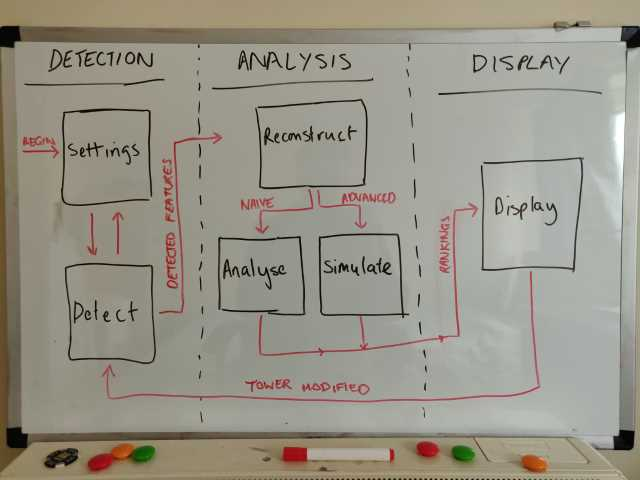
\includegraphics[width=0.6\linewidth]{images/design/architecture}
    \caption{System Architecture}
    \label{fig:architecture}
\end{figure}

\subsubsection{Settings}

When entering the system (top left of \cref{fig:architecture}) the user must begin with configuring settings for the application. These settings include items such as the number of blocks to detect, which analysis method to use, and how to display the results.

\subsubsection{Detection}

After the user has configured settings, the flow of the application should move into the detection stage. Here the user can use their camera, likely on the back of their phone, to scan and detect the blocks. The method used to detect the blocks will be marker based, which means that the user needs to move around the tower with their camera to detect each block individually, the benefits of using this method are described later in \cref{sec:des:detection}. During the detection, the user should be able to move back into the settings screen, in the case that their settings are causing the blocks to be inaccurately detected, or move onto the analysis stage.

\subsubsection{Reconstruction}

The analysis stage, shown in the centre of the figure separated from other stages with vertical dotted lines, is accessed from the detection stage by passing detection data, indicated by a red, arrowed line labelled \textit{Detected Features}.  Without delay (\cref{req:realtime}), the system should use these data to reconstruct the real world tower in three-dimensional virtual space; this could be done by instantiating block objects between markers on end faces of each block,  which is a parts-based modelling approach. Two arrows then emerge from the reconstruction section, moving into the naive or the advanced analysis method respectively.

\subsubsection{Heuristics}
If the user has chosen to use the \textit{naive} analysis approach, then the system will use a set of rules to determine the block removal feasibilities (\cref{req:rank}), and this includes rules such as the following that will be expanded upon later:
\begin{itemize}
    \item Set any blocks which singularly occupy their layer to have a low removal feasibility
    \item Set any central blocks which are neighbouring two side blocks to have a high removal feasibility
\end{itemize}

\subsubsection{Simulation}

Alternatively, the system will move into the simulation section in which the virtual tower is subject to numerous physics simulations to more accurately predict block removal feasibility. An example of the simulations used is to remove a block, then waiting a specified amount of time to test whether or not the tower remains stable, followed by resetting the tower state and iterating through the remaining blocks, resulting in a stability score for each block.

\subsubsection{Visualisation}

To end with, the \textit{Rankings} arrow shows movement between the analysis and display stages. Rankings, otherwise referred to as block removal feasibility rankings, are received and displayed in the format chosen by the user earlier, in the settings screen. Methods for display should include augmented reality (\cref{req:augment}), and can include \jenga{} variations (\cref{req:variants}), such as challenges, handicaps, and a points system.

The display stage should also allow the user to enter back into the detection stage (see \textit{tower modified} arrow at the bottom of \cref{fig:architecture}) because the real-world tower will eventually be modified by the user, rendering the current analysis useless, so the system state will need recalculating.

\section{\detection}\label{sec:des:detection}

Now that an overall architecture has been proposed, the method for the marker-based detection must be refined. Please refer to \cref{sec:markerless} for analysis into why marker-based was chosen over markerless detection, and \cref{code:houghpy} for the short program written to validate a markerless detection method. It has already been established (\cref{subsec:detectionsummary}) that UcoSLAM is the most appropriate method for the detection of blocks in a camera frame, but there is still a critical design choice that needs to be made, namely how exactly to affix markers to the blocks.

\subsection{Marker Affixation}\label{sec:markeraffixation}

\citet{arucopaper} explain that the smaller the marker, the more prone it is to errors during detection, however original \jenga{} blocks have faces that are just 15mmx25mm in dimensions, meaning that a margin of error cannot be avoided. To minimise the potential for errors, the markers must be as large as possible on the face, without being so large as to confuse the detection algorithm between multiple close-by markers.

\cref{fig:markersonblocks} shows one way to affix markers to blocks in this project, in which square, double-sided, sticky pads were used. This solution is advantageous because sticky pads and paper-printed markers are cheap to acquire, and simple to apply. However, the operation of attaching 108 pads and markers is a tedious task, which means that it has low commercial viability as users are unlikely to want to attach markers to their blocks in this way. Despite this, the markers were detectable using the ArUco test executable, as shown in \cref{fig:markersonblockswithposes}, in which the three axes and a box are drawn around the detected markers.

\begin{figure}[ht]
\centering
\begin{minipage}{0.45\textwidth}
  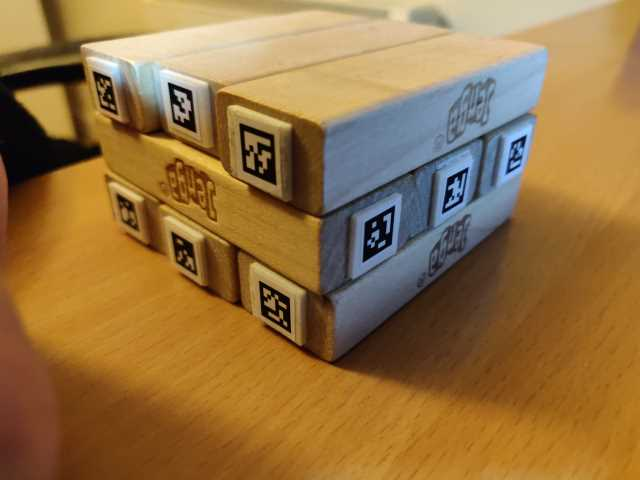
\includegraphics[width=\linewidth]{images/design/markersonblocks}
  \caption{Markers stuck to blocks}
  \label{fig:markersonblocks}
\end{minipage}
\begin{minipage}{0.45\textwidth}
  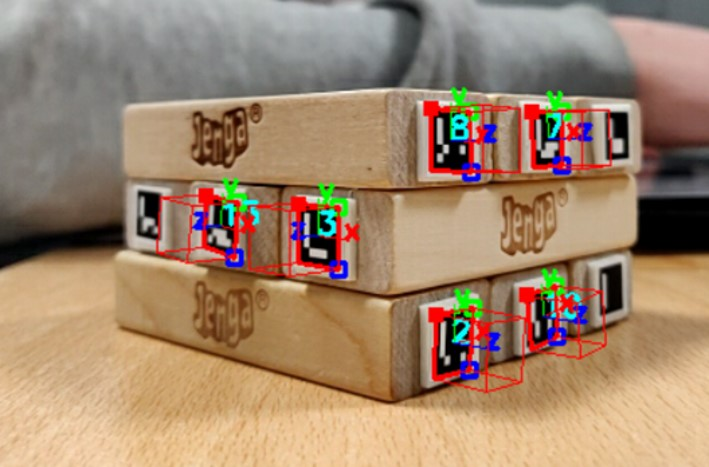
\includegraphics[width=\linewidth]{images/design/markersonblockswithposes}
  \caption{Detected poses and boxes}
  \label{fig:markersonblockswithposes}
\end{minipage}
\end{figure}

Another way to affix markers to blocks is by using a laser cutter. To do this, the blocks can either be cut individually, all together at once, or at some point in between the two. The benefit of cutting the blocks individually is that it is easier to centre the block under the laser to ensure the marker is cut in the middle, which increases the minimum distance between markers on separate blocks, yet this method is just as monotonous as using sticky pads. Also, any blocks which have misaligned marker placement could be thrown out at the loss of just one block each time.

Conversely, cutting all the blocks at once allows for significantly less cutting time, but brings about the risk of misalignment on multiple blocks at a time, coincidentally this did happen and can be seen in \cref{fig:misalignment}. The slight variations in block sizes, multiplied by the number of blocks bound together, meant that rows of the bound blocks were misaligned, hence the laser cut in the wrong places. In addition to this problem, the laser cutter used did not have any in-built alignment tools, so blocks had to be positioned by hand, leading to human error.

\begin{figure}[ht]
\centering
\begin{minipage}{0.45\textwidth}
  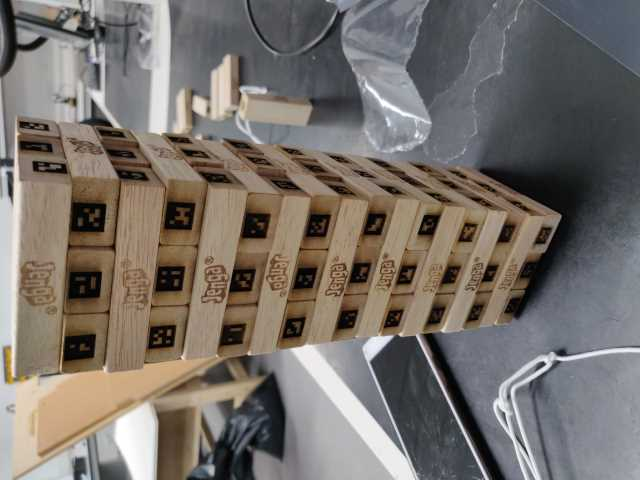
\includegraphics[width=\linewidth]{images/design/misalignment}
  \caption{Misalignment during the cutting process}
  \label{fig:misalignment}
\end{minipage}
\begin{minipage}{0.45\textwidth}
  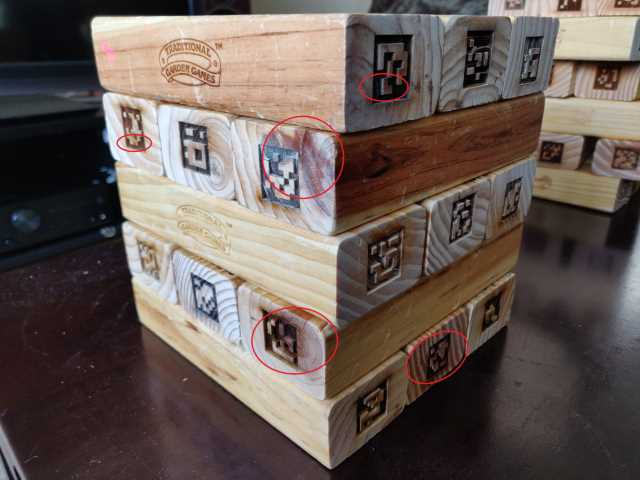
\includegraphics[width=\linewidth]{images/design/largeblocks}
  \caption{Large blocks with markers, red circles indicate colour variation}
  \label{fig:largeblocks}
\end{minipage}
\end{figure}

After several attempts and various methods of aligning blocks in the laser cutter it was decided that such a task was too difficult to accomplish to the degree of precision needed. A solution to this was to use blocks of greater size, this is because the faces of the larger blocks could allow for relatively smaller markers, thus reducing the risk of misalignment. Still, there were problems. The big blocks used had different wood grain and texture, leading to variations in colour and brightness, these are pointed out in \cref{fig:largeblocks}, and due to this, some blocks were unable to be detected by the ArUco library.

In summary, affixing markers to blocks is not as straightforward as it would seem and no method was found to have both ease of setup and low error rate. Despite this, the sticky pad and paper method should be adopted for the implementation because of its success in low error detection.

\section{\analysis}

Moving forward, the analysis stage must be addressed. Following \cref{req:rank}, this stage has to use the detected features data to reconstruct the tower in a virtual space, and then calculate rankings for block removal feasibility for later display. This section details design choices made for both \nameref{subsec:heuristics} and \nameref{subsec:simulation} analysis.

\subsection{Heuristics}\label{subsec:heuristics}

One way in which to approach the analysis problem is to use a set of simple rules to determine block removal feasibility rankings, these are described below, with reasons given as to why they were chosen. In the rule set, it is assumed that there are three blocks per layer, referred to as two side blocks, and one central block. Also, the red cross in the diagrams show which block is to be removed.

\begin{enumerate}
    
	\item \textbf{Constraint:} Any block which singularly occupies its layer.
	\\\textbf{Feasibility of removal:} Low.
	\\\textbf{Reason:} All above layers would fall by one block height, which adds risk if the tower is already unstable.
	
	 \begin{figure}[ht]
        \centering
        \begin{minipage}{.3\textwidth}
            \centering
            \drawblockrow{1}{}{}{1}
        \end{minipage}\hfill
        \begin{minipage}{.3\textwidth}
            \centering
            \drawblockrow{}{1}{}{2}
        \end{minipage}\hfill
        \begin{minipage}{.3\textwidth}
            \centering
            \drawblockrow{}{}{1}{3}
        \end{minipage}
        \caption{Possibilities for Rule 1}
    \end{figure}
	
	\item \textbf{Constraint:} Any side block which is situated on a layer with only one other side block.
	\\\textbf{Feasibility of removal:} Low.
	\\\textbf{Reason:} The above layers would pivot around the remaining side block, causing the tower to fall.
	
	\begin{figure}[ht]
	\centering
	\begin{minipage}{.45\textwidth}
        \centering
        \begin{minipage}{.45\textwidth}
            \centering
            \drawblockrow{1}{}{1}{1}
        \end{minipage}
        \begin{minipage}{.45\textwidth}
            \centering
            \drawblockrow{1}{}{1}{3}
        \end{minipage}
        \caption{Possibilities for Rule 2}
    \end{minipage}
    \begin{minipage}{.45\textwidth}
        \centering
        \begin{minipage}{.45\textwidth}
            \centering
            \drawblockrow{1}{1}{}{1}
        \end{minipage}
        \begin{minipage}{.45\textwidth}
            \centering
            \drawblockrow{}{1}{1}{3}
        \end{minipage}
        \caption{Possibilities for Rule 3}
    \end{minipage}
    \end{figure}
	
	\item \textbf{Constraint:} Any side block which is situated on a layer with only one other central block.
	\\\textbf{Feasibility of removal:} Medium.
	\\\textbf{Reason:} The centre of mass of the above layers is usually near the middle of the tower, so this side block is unlikely to be bearing weight.
 	
 	\item \textbf{Constraint:} Any central block which is situated on a layer with only one other side block.
    \\\textbf{Feasibility of removal:} Low.
    \\\textbf{Reason:} The above layers would pivot around the remaining side block, causing the tower to fall.
	
	\begin{figure}[ht]
	\centering
	\begin{minipage}{.6\textwidth}
        \centering
        \begin{minipage}{.45\textwidth}
            \centering
            \drawblockrow{1}{1}{}{2}
        \end{minipage}
        \begin{minipage}{.45\textwidth}
            \centering
            \drawblockrow{}{1}{1}{2}
        \end{minipage}
        \caption{Possibilities for Rule 4}
    \end{minipage}
    \begin{minipage}{.3\textwidth}
        \centering
        \begin{minipage}{0.9\textwidth}
            \centering
            \drawblockrow{1}{1}{1}{2}
        \end{minipage}
        \caption{Rule 5}
    \end{minipage}
    \end{figure}
	
	\item \textbf{Constraint:} Any central block which neighbours two side blocks.
	\\\textbf{Feasibility of removal:} High.
	\\\textbf{Reason:} Neighbouring side blocks act as stabilisers.
	
	\item \textbf{Constraint:} Any side block situated on a full layer.
	\\\textbf{Feasibility of removal:} Medium.
	\\\textbf{Reason:} The centre of mass of the above layers is usually near the middle of the tower, so this side block is unlikely to be bearing weight.
	
	\begin{figure}[ht]
        \centering
        \begin{minipage}{.3\textwidth}
            \centering
            \drawblockrow{1}{1}{1}{1}
        \end{minipage}
        \begin{minipage}{.3\textwidth}
            \centering
            \drawblockrow{1}{1}{1}{3}
        \end{minipage}
        \caption{Possibilities for Rule 6}
    \end{figure}
	
\end{enumerate}

This method is good because it is simple to implement, and also has low complexity and runtime. However, it assumes the blocks will be aligned with the tower in the same way that they were in the starting state, yet it is likely that the blocks will rotate and translate from their original positions as the game progresses, meaning that this analysis would lose truth with changes to the tower state, thus providing a poor estimate for ranking.



\subsection{Simulation}\label{subsec:simulation}

A more advanced method for analysis would be to use physics simulation software, which allows developers to implement the laws of physics into their applications. Simulation software could be used to determine more accurate removal feasibility rankings than the \nameref{subsec:heuristics} method because it takes into account more advanced physics features, thus adding realism to the analysis. In this section, two physics simulators, Unity and Project Chrono, are compared, before the design for the simulation program is described.

\subsubsection{Software}

\cite{projectchrono} is an open-source physics engine specialised for use with robotics and biomechanics, but is capable of supporting much more. Advantages to using Chrono are that it is highly customisable, with realistic physics, and can be compiled to Android (\cref{req:android}). On the other hand, it has a steep learning curve and is not natively packaged with a GUI.

In contrast, \cite{unity} is primarily a game engine that runs on the PhysX engine. It also brings native support for Android, but does come with a built-in GUI that has drag and drop functionality and is easy to get started with. In addition, Unity has a large community with lots of support and wikis, which means that there will be people to whom to turn if problems are encountered. It is because of these benefits over Chrono that it was decided to use Unity for the simulation software.

\subsubsection{Simulation Design}

After deciding to use Unity as the software for simulation, the next step is to decide what will take place in the simulations, and how to score the removal feasibility rankings for each block.

The first, and simplest way to do this is to build the tower from the block poses, then systematically remove each block and calculate whether or not its removal causes the tower to fall over. To calculate is the tower is left standing, the simulation could wait a specific amount time, and then check if the highest block is still at the same level that it was before block removal. This method gives a good indication of the vitality of each block with regard to tower stability, however, it only produces binary output; \textit{fallen} or \textit{standing}, and it could also give a \textit{fallen} result if a whole row is removed at once, which is a legal move in the game. Furthermore, it does not consider the movement of the removal block, as it will just be destroyed in position, which means that it ignores real-world factors such as rotation and friction.

The above method can be improved by giving a more distributed score for the set of blocks. This could be done by either calculating the time it takes for the tower to fall, and using that value to scale the results. Another way involves waiting a fixed amount of time after removal, and then finding out how far the furthest block has travelled from the centre of the tower. Both of these techniques would produce a similar outcome, and so they should be tested in the \nameandsecref{chap:implementation}.

Moreover, it could also be improved by changing the way blocks are removed from the tower. Instead of destroying each block in place, the simulation could attempt to pull the block out from the tower. There are a few constraints on how it is possible to remove blocks from a tower while trying to minimalise disturbance \citep{jengaanalysis}; central blocks can only be moved perpendicularly to the tower, whereas side blocks can be removed by rotation or translation away from the tower. This may prove difficult to simulate because the previous work done in this area showed that finding the correct physics properties for realistic block removal is no easy task, nonetheless, effort should be made to implement this later on, as removing the blocks in this way provides a more accurate representation of how they would be removed in the real world.

\begin{figure}
    \centering
    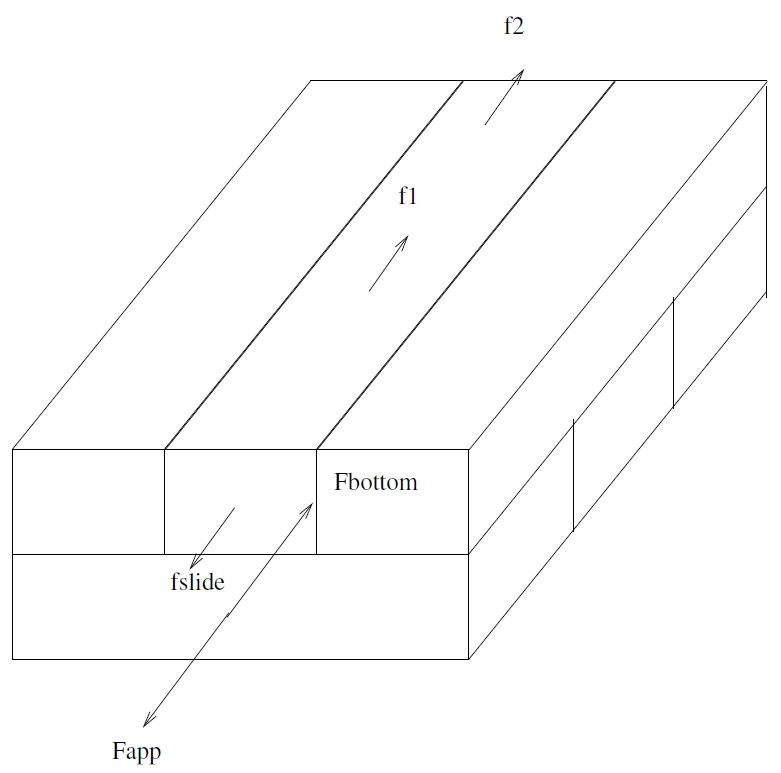
\includegraphics[width=.4\textwidth]{images/design/analysisjengamovement}
    \caption{Central block removal, image from \citet{jengaanalysis}}
    \label{fig:centralblockremoval}
\end{figure}

\section{\display}

Designing the visualisation stage is subsequent to finalising designs for detection and analysis. This section aims to cover both what to display (\cref{subsec:variation}) and how to display (\cref{subsec:tools}) the removal feasibility rankings to the user.

\subsection{Tools}\label{subsec:tools}

There are various tools and kits available for augmented reality display, of which, ARCore and OpenCV are two of the most prominent at this time. Solutions using these software are described below.

\subsubsection{ARCore}

ARCore is an augmented reality software development kit built for Android smartphones, similar to ARKit for iOS smartphones, that can be paired with other software such as Unity for extensibility. One solution using ARCore includes using the virtual tower built earlier in Unity, and displaying that on the phone screen. With ARCore it is possible to track the environment and place virtual objects directly onto planes, the solution should make use of this feature by allowing the user to generate the virtual tower on the same plane that the real tower is occupying. Having the two towers side by side means that the user can compare them efficiently, which satisfies \cref{req:stageunderstand} for ease of use.

\begin{figure}[ht]
\begin{minipage}{\textwidth}
    \centering
    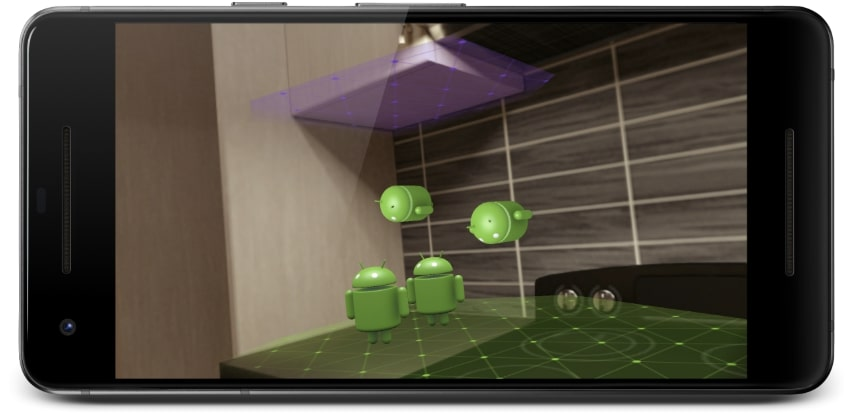
\includegraphics[width=.8\textwidth]{images/design/andyandroid}
    \caption{An example of using ARCore to place virtual objects onto a real plane, image from this  \protect\footurl{https://developers.google.com/ar/develop/unity/quickstart-android}{ARCore Sample}}
    \label{fig:andyandroid}
\end{minipage}
\end{figure}

Another way to display the tower with ARCore is to place the virtual tower directly on top of the real tower so that only the virtual tower is visible. Doing this provides a more immersive experience to the user, which means that they are less likely to lose attention (\cref{req:attention}). However, ARCore does not allow for tracking of multiple individual objects, so when the user tries to take a block from the tower, only the physical piece will be removed, leaving the virtual in its place; this may be unexpected behaviour to the user and could result in confusion, which is detrimental to the success of the system.

\subsubsection{OpenCV}

Alternatively, OpenCV could be used for the display. While the previously mentioned method pairs well with Unity, this software goes hand in hand with augmented reality markers, which are already affixed to the blocks. The advantage of this method is that it can track the individual markers, meaning that the experience does not have to end when a block gets removed; it provides dynamic augmentation even during the process of removal, unlike the ARCore method.

\subsubsection{Virtual}

On the other hand, a solution exists without the use of AR, that is to present the information in virtual reality. Again, this method uses Unity, but instead of placing the virtual tower into the real environment, it stays on screen, with the ability to zoom in on different areas of the tower, and rotate to see other sides. However, when compared with the methods as mentioned earlier, this is less immersive and requires more work for the user; therefore it should not be used in the implementation.

\subsubsection{}
In summary, OpenCV should be the method of choice for displaying the results because it tracks the individual blocks at all times, contrary to the ARCore method. Yet, it would still be worthwhile to incorporate ARCore into the system as an extension, if time allows for it at the end of the project.

\subsection{Variation}\label{subsec:variation}
In this project, it would be adequate to take the raw block removal feasibility rankings and augment those numbers onto each block. While this would serve the purpose of the system, it may be beneficial to implement additional variations for reasons of aesthetics and increased gamification.

The method used to capture design solutions for these variations was brainstorming. Various ethics were considered before participants were engaged in this study, details of which can are in \cref{chap:ethics}. This section explains what each leaf of the mind-map in \cref{fig:brainstorm} represents:

\begin{figure}[ht]
  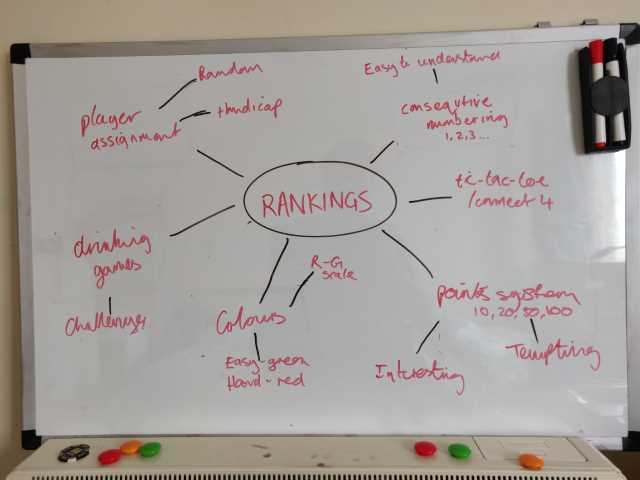
\includegraphics[width=\linewidth]{images/design/rankings}
  \caption{Brainstorm of game variants}
  \label{fig:brainstorm}
\end{figure}

\subsubsection{Consecutive Numbering}
The first variation considered was also the most blatant: consecutive numbering. In short, this means that the ranking should be displayed as is, beginning from 1, meaning most feasible to remove, and traversing through all the blocks to the least feasible, adding one to the counter at each block. This method is arguably the easiest to understand, and gives the user clear indication of the block ranks, although it lacks visuals, and therefore it would be less interesting than competing methods.

\subsubsection{Points System}
Extending from the consecutive numbering method is the points system; it differs from the numbering method as blocks are assigned ranks in bands. For instance, high feasibility blocks are designated to have 10 points, medium feasibility have 20 points, and low have 50 points. When a user removes a block, they receive the number of points that the block is worth, intending to end the game with the most points out of all players. This method is well-suited to \jenga{} because it adds an extra variable in consideration of which block to choose, making the game more interesting. Also, a 100 point band could be used for blocks which are deemed improbable to remove, tempting the more risk-averse players in for more points.

\subsubsection{Colours}
Maybe the most visual of the variants that evolved from the brainstorm is the colour variant, in which blocks are coloured based on their rank. Two ways this could be completed are by using a colour scale, or colour bands. The colour scale is a smooth transition from red to green, indicating the hardest and easiest blocks to remove respectively, which would be useful to the user as colours are good visual cues. On the other hand, colour bands could be used, for instance, red for difficult blocks, yellow for medium blocks, and green for easy blocks. Out of the two methods, the colour scale is preferred because it gives more information to the user.

\subsubsection{Tic-Tac-Toe / Connect 4}
An interesting suggestion was to incorporate minigames, such as tic-tac-toe and connect 4. Players work in teams to either pull out a certain number of blocks in a row, which would be 3 in the case of tic-tac-toe, or 4 in the case of connect 4. The visualisation for these variations is opposite to the ones already mentioned because they require the empty gaps to be augmented, which is more difficult to implement because the system does not implicitly know where gaps are in the tower.

\subsubsection{Player Assignment}
Moving to the left of \cref{fig:brainstorm}, is player assignment, this is where blocks are assigned to specific players at the start of the game, and players are restricted to only remove blocks assigned to them. Extending on this idea, the player assignments can be dynamic throughout the game, changing to give the harder blocks to the top players, as a handicap feature. This variant is worth considering because it makes the game more personal, which means that players are more likely to feel included.

\subsubsection{Challenges}
Finally, a drinking variant was proposed. After this suggestion, the study participant was advised that variants should be targeted towards all audiences, not just a specific group, such as those who drink alcohol; resulting from this, the variant was named \textit{Challenges} instead. The challenges variant involves assigning various tasks to each block at the start of the game, such as doing a star jump, or naming 5 capital cities. What is good about this variant is that the set of challenges are endless, and could even be set by the users, meaning that they can choose appropriate tasks for their player group.

\subsubsection{Summary}\label{sec:variantssummary}
The brainstorming activity was a success because the participants came up with six unique variants that could all be implemented into the system, which is more than was hoped for. Moving forward, the colour variant should be the first to be adopted, due to its pleasing aesthetics (\cref{req:aesthetics}), but other variants should not be forgotten about, and could be worked towards as an extension to the project.

\section{System}

The final section in this design chapter involves the overall system design and interface. It begins will an 

\subsection{Standalone}\label{sec:standalone}

Initially, a solution was white-boarded to achieve a quick and simple design, shown in \cref{fig:handdrawngui}. The Settings screen (left) contains only a few items; an input box for the number of blocks, a dropdown box to select the marker dictionary, and a button to move onto the Camera screen. An effort was made here to keep the design both simple and minimal, because too much information leads to poor design. Furthermore, the Camera screen (right) contains but two items, a full screen camera and a button to return to the Settings, these were chosen to aid in the immersion of the application.

\begin{figure}[ht]
\begin{minipage}{0.45\textwidth}
    \centering
    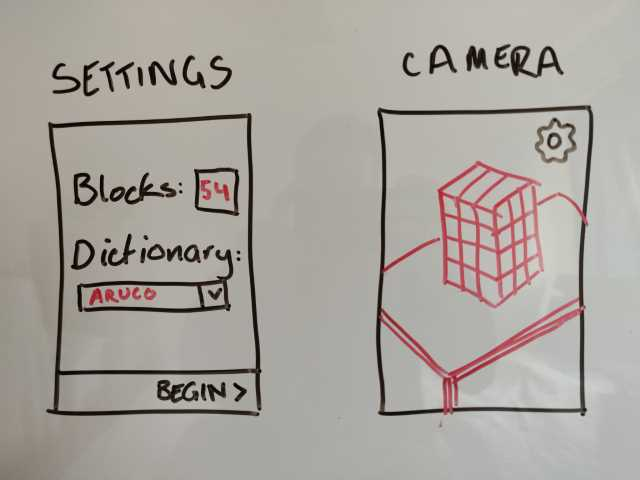
\includegraphics[width=0.9\textwidth]{images/design/gui}
    \caption{Hand-drawn}
    \label{fig:handdrawngui}
\end{minipage}\hfill
\begin{minipage}{0.45\textwidth}
    \centering
    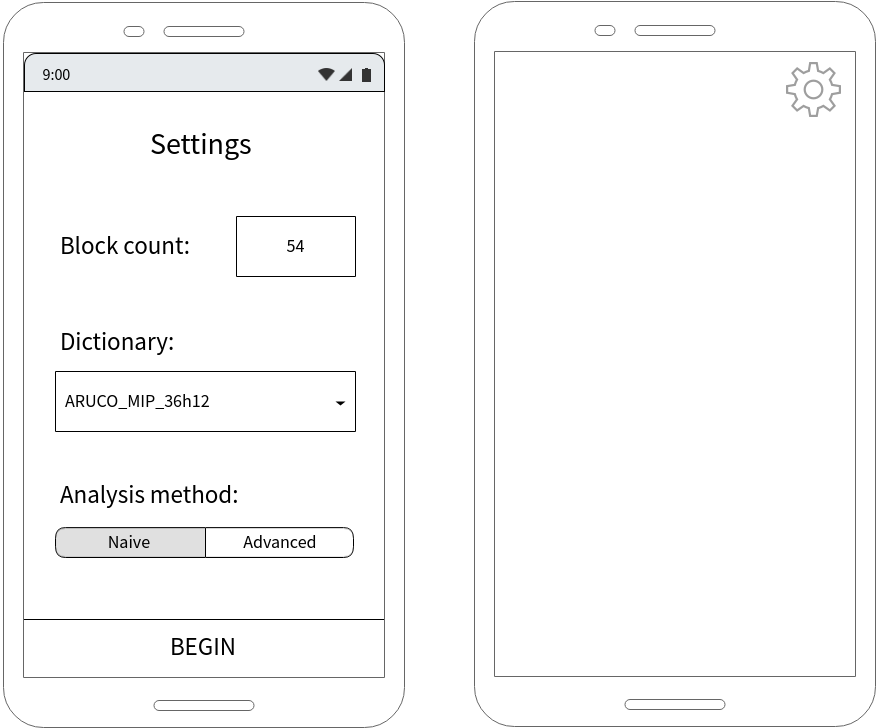
\includegraphics[width=0.9\textwidth]{images/design/wireframe}
    \caption{Wire-frame}
    \label{fig:wireframe}
\end{minipage}
\caption{Graphical User Interfaces}
\label{fig:gui}
\end{figure}

To formalise and improve the system design, a wire-frame model was created using the white-boarded solution as a template. Several changes were made to the settings, these were the addition of the analysis method, as well as a title, and centring the Begin button. With these changes, the design looks cleaner, and includes more of the desired functionality of the system. In contrast to the changes made to the Settings screen, there were no changes to the design of the Camera screen, this is because the design is minimal enough to include all the needed functionality, but not so little to cause confusion. For example, the Settings button could be removed in favour of a swipe action and to allow for a truly fullscreen camera, but some users would then find it difficult to navigate to the settings.

\subsection{Server / Client}

The documentation for \citet{ucoslam} states that one of the main features is:

\begin{displayquote}
\textit{``Multiplatform, ready to be compiled in Windows, Linux and Android systems''}
\end{displayquote}

However, several attempts to compile the library for Android failed. The approaches taken were widely varied, but including using different operating systems, i.e. Ubuntu 16, Ubuntu 18, and Windows 10, downgrading Android build tools, building older versions of OpenCV, compiling with legacy versions of the Android NDK, and various CMake option changes. On top of this, the developer of UcoSLAM was reached out to, but no response was received before the hand-in date. So, although the documentation claims to be ready to be compiled for Android systems, this was found not to be possible; thus a different system design had to be conceived.

The solution to the compilation problem in this paper is to switch from a standalone architecture to a client/server architecture, this is done in such a way that the client sends camera frames to the server which performs the localisation and mapping of markers, and then the server sends results back to the client. Developing the application in this way means that the software used to map markers is not restricted to running on a smartphone, which means that UcoSLAM can still be used in the project.

It is worth noting that changing to this architecture partially violates \cref{req:android} because part of the application now runs on a server, instead of an Android device, but there are significant advantages which outweigh this requirement violation. For instance, complexity has been removed from the Android app, meaning that it will be easier to maintain. Also, now there is an opportunity to move the analysis stage onto the server, which means that less compute heavy tasks need to run on the device, opening up the application to devices with slower hardware (\cref{req:lightweight}). With the analysis stage on the server, more complex simulations can be run, giving the potential for more accurate feasibility rankings, which improves on \cref{req:accuracy}.

\begin{figure}[ht]
    \centering
    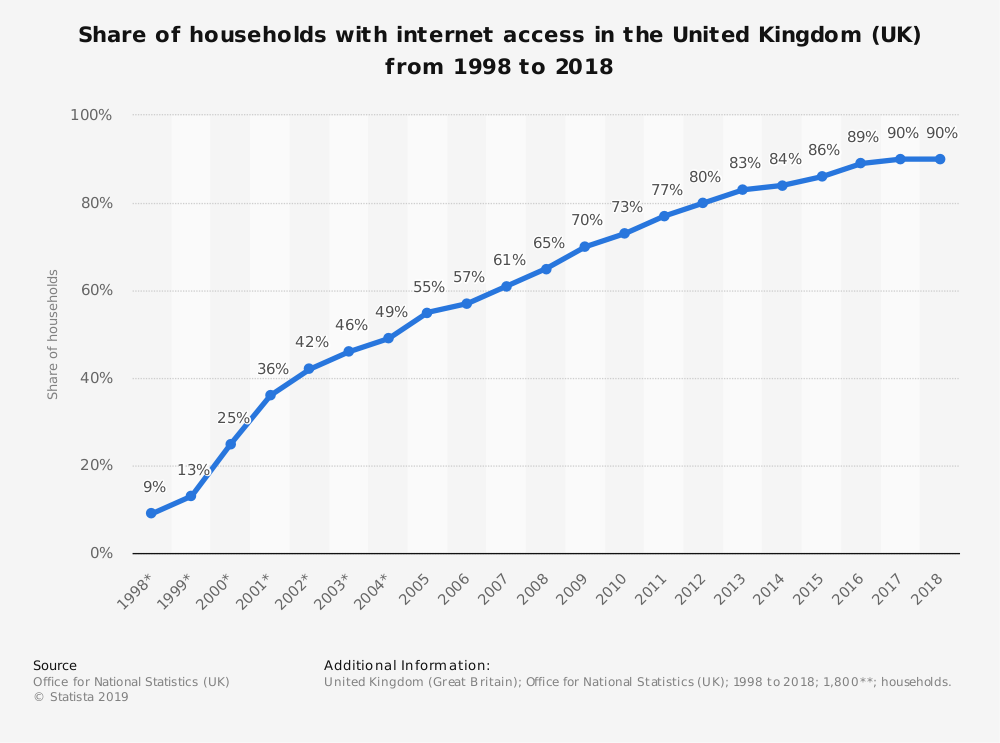
\includegraphics[width=.6\linewidth]{images/design/homeswithinternet}
    \caption{Households with internet access in the United Kingdom (UK), image from \cite{internetaccess}}
    \label{fig:internet}
\end{figure}

Disadvantages of the client/server approach include the need for a server to be present during the runtime of the application, this means that users are constrained to only using the app when they have a working internet connection, or can use a local server, such as a laptop or PC. However, today, this will generally not be an issue due to widespread internet access, for example, \cref{fig:internet} shows that 90\% of homes in the UK have access to the internet. Furthermore, adding a server into the system adds overall complexity, because inter-device communication has to be implemented.

\subsubsection{Changing Requirements}\label{subsec:changingrequirements}

Requirements were previously set under the assumption of a standalone system, but as a result in the change of architecture, new requirements were set and can be found in \cref{sec:req:additional}. One of the most crucial additional requirements (\cref{req:comms}) is that the communication with the server must be asynchronous, this means that a separate thread will be used to send and receive data, which is beneficial because the application will not be blocked from running when it decides to send a frame to the server. If the communication were blocking, then the camera activity in the app would seem jittery, as the screen would only update after completing send to the server, which can take an arbitrarily long time.

Another cause for concern, indicated by \cref{req:privacy}, is privacy. It is not unreasonable to assume that some images sent from the smartphone app will contain personal information, for example a postal item which contains the name and address of the user. For this reason, the server must not store any of the images it receives from a client, this is possible if frames are processed immediately and then thrown away when after pose information has been extracted.

\subsubsection{Design}

A high level overview of the responsibilities of the client and server is shown below in \cref{fig:clientserverarch}.

\begin{figure}[ht]
    \centering
    \begin{minipage}{.45\textwidth}
        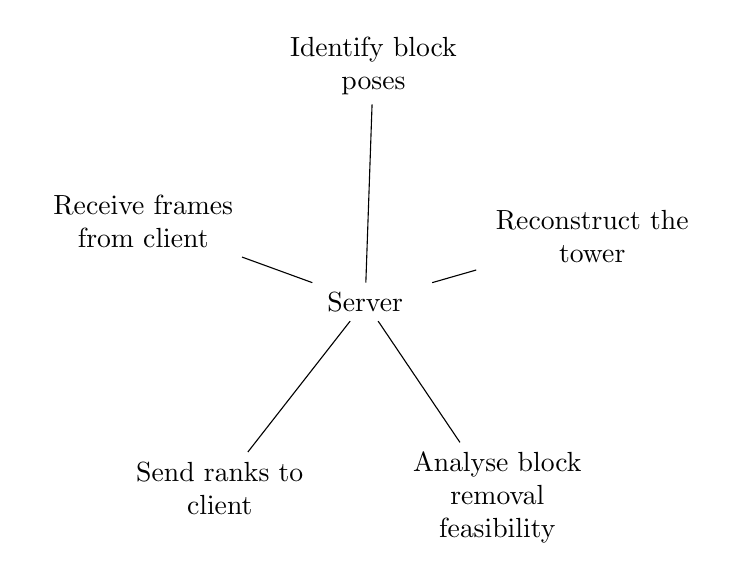
\begin{tikzpicture}[grow cyclic, text width=2.7cm, align=flush center,
        	level 1/.style={level distance=3cm,sibling angle=72}]
         
        \node{Server}[clockwise from=160]
            child { node {Receive frames from client}}
            child { node {Identify block poses}}
            child { node {Reconstruct the tower}}
            child { node {Analyse block removal feasibility}}
        	child { node {Send ranks to client}};

        \end{tikzpicture}
    \end{minipage}\hfill
    \begin{minipage}{.45\textwidth}
        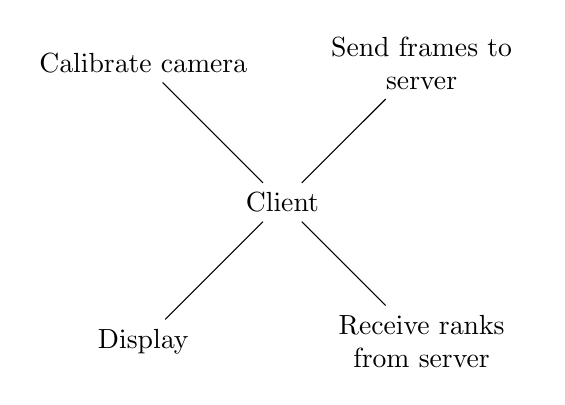
\begin{tikzpicture}[grow cyclic, text width=2.7cm, align=flush center,
        	level 1/.style={level distance=2.5cm,sibling angle=90}]
            \node{Client}[clockwise from=135]
            	child { node {Calibrate camera}}
            	child { node {Send frames to server}}
            	child { node {Receive ranks from server}}
            	child { node {Display}};
        \end{tikzpicture}
    \end{minipage}
\caption{High level responsibilities}
\label{fig:clientserverarch}
\end{figure}

\section{Summary}

This chapter has described and explained the design choices for the system. Next, this system will be implemented.
%---=---==---===---====---=====---======---=====---====---===---==---=---%
%-                  DETAILED DESIGN AND IMPLEMENTATION                  -%
%---=---==---===---====---=====---======---=====---====---===---==---=---%

\chapter{Implementation}\label{chap:implementation}

The implementation chapter involves taking the design choices made previously, and implementing them into the system. Sections covered are networking, detection, analysis, visualisation and interfacing, with each detailing how the implementation was completed. Code snippets and images are presented throughout to better explain some of the more crucial steps, however refer to the \nameandsecref{chap:code} for viewing the full code base.

\section{Networking}
The most important functions to implement for network communication are for sending and receiving data. \citet{boost} is a set of C++ libraries that support a number of tasks such as multithreading and image processing, it is also capable of cross-platform networking, and thus could be used solve the communication problem in this project. However, dependencies on libraries can bring up problems, such as complicating cross-platform building, and larger package sizes, so in an effort to keep the networking implementation small, it was decided to write the networking functions without the use of a library.

\cref{lst:recv} shows several lines of the receive function that was implemented, it takes a generic buffer, an integer length, and a number of retries as parameters. Using generics in this function makes the code more robust because it means the system has the ability to send any buffer type, for example, strings, unsigned chars and integers. Also, the function makes use of exponential backoff (\cref{lst:expbackoff}), which means that if the system attempts to send a buffer that does not get received on the other end, it will wait an ever growing amount of time before trying again. Exponential backoff is beneficial to the system because it prevents unnecessary resources from being used up when the connection between nodes is not fully realised. A backoff limit of 10000ms was chosen as it is long enough to not cause resource issues, but not too long as to cause inconvenience to the user.

\lstinputlisting[style=cpp, linerange={30-37}, label={lst:recv}, caption={Receiving network bytes in \nameandsecref{code:network}}]{code/network.hpp}

\lstinputlisting[style=cpp, linerange={51-53}, label={lst:expbackoff}, caption={Exponential backoff in \nameandsecref{code:network}}]{code/network.hpp}

In contrast, the send function (\cref{lst:send}) sends all bytes from a generic buffer. It does this by attempting to send the whole buffer at once, if the whole buffer is successfully sent in one transaction then the function returns, otherwise, if the amount of bytes sent is less than the buffer size, then the function will attempt to send whatever data is remaining, this is useful for sending large buffers of data which exceed the network protocol maximum segment size, such as images. On the other hand, if an attempt fails because the socket does not contain an open connection, the function will throw a SocketException, which will print an error such as "Failed to send all bytes of message. 4/12 of char array.". This error type was useful for debugging when writing the network functionality, because it gives the programmer a detailed description of what was being sent when the error occurred, and will continue to be useful when network problems occur in the future.

\lstinputlisting[style=cpp, linerange={59-66}, label={lst:send}, caption={Sending network bytes in \nameandsecref{code:network}}]{code/network.hpp}

Next, \textit{send} and \textit{receive} can be built on top of to create more appropriate functions, like sending and receiving images. Images in OpenCV are stored in matrices, which have a number of rows, columns and channels, for instance, an HD coloured image may be stored as a 1080x1920x3 matrix of unsigned chars. Sending a matrix first requires encoding to the Portable Network Graphics (PNG) format, which supports lossless data compression, this is good because compressed files take less time to send over a network than their sources, and also no data is lost, unlike competing compression methods such as JPEG. Then, the PNG buffer size is sent to the receiving node, so that it knows how large the matrix will be, and then finally the buffer itself is sent. On the receiving node, a simple decode of the data is required to convert back to the matrix type.

Unfortunately, compiling OpenCV with encoding functionality was not possible because of an undefined reference in the SDK, so a compromise was made which involved sending the raw matrix as continuous data, and reconstructing that matrix on the other side. This method is slower than when using compression, and therefore should only be used when the OpenCV \textit{imencode} and \textit{imdecode} functions are unavailable, like with the Android SDK.

The next step after creating the functionality for sending matrices is to handle when and how to begin communication between client and server. For instance, if the client needs to send data, then it should know that the server is ready to receive the required type of data, for this, aptly named functions \textit{sendTypeOfData} and \textit{getTypeOfData} were created. As the functions are generic, they allow for any continuous data type to be transfered, but for sake of example the list below shows the implemented process for sending an integer to the server:

\begin{enumerate}
	\item Nodes establish a connection with each other
	\item Server waits on a data type to be received
	\item Client sends the \textit{int} type to the server
	\item Server receives the \textit{int} type
	\item Server checks whether the current state of the system allows for an \textit{int} to be received
	\begin{enumerate}
		\item If an \textit{int} is acceptable, then server sends a \textit{GOOD\_REQUEST} status to the client
		\item Else, server sends a \textit{BAD\_REQUEST} status, followed by a list of valid request types, then returns to step 2
	\end{enumerate}
	\item Client sends the value of the \textit{int} to the server
	\item Server receives the \textit{int} value
	\item Server performs necessary computation with the received value
\end{enumerate}

Implementing the inter-node communication in the above way has several benefits over just sending data and hoping that it is well received on the other side. One of these reasons is that the server can validate requests, which is useful when it is expecting certain types of data, for example before the server perform localisation and mapping on camera frames, it first needs to know the camera calibration coefficients (more on this later in \cref{calib}). Therefore, if the client tries to send image data before sending its camera calibration, the server can choose to not accept that data, and notify the client that its request was unfounded. On top of this, the implementation is extendable (\cref{req:extendable}) by simply adding to the list of valid data types and implementing a function to perform on receipt of that data type.

Finally, sending images is a time-consuming task, as discussed in \cref{subsec:changingrequirements}, and must be performed asynchronously to satisfy \cref{req:comms}. In the implementation, this is done using \possessivecite{readerwriterqueue} ReaderWriterQueue library, which includes just two C++ header files that provide a single-producer, single-consumer lock-free queue. This library was used because of its compactness, and also since implementing multi-threaded operations is an incredibly subtle task, for instance, bugs can remain unseen in several runs of an application, only to appear seemingly out of nowhere later on. Using ReaderWriterQueue ensures that the operations are thread-safe because they have been tested and validated by the open source community. Now when the main thread of the client wants to send an image, it pushes that image to a queue and then immediately continues with its other tasks. At the same time, a worker thread checks the queue, and sends any new frames over to the client, thus providing the necessary asynchronous operation.

\section{\detection}
\subsection{Calibration}\label{calib}

With the client/server implementation completed, the next stage to implement is marker detection and pose estimation (\cref{req:pose}), but before marker poses can be estimated, camera-specific distortion must first be addressed (\cref{req:camera}). The implementation for which is as follows:

\begin{enumerate}
	\item Generate and print an ArUco or ChArUco board
	\item User is directed to point the camera towards the board
	\item System detects markers in each camera frame
	\begin{enumerate}
		\item If more than half of the board markers are detected, save the marker id and coordinates
		\item Otherwise, disregard the frame
	\end{enumerate}
	\item When markers for at least 10 images have had their marker coordinates saved, calibrate the camera
	\item Finally, send calibration details to the server
\end{enumerate}

The above implementation builds in two variables that are different from the standard calibration process. Firstly, the number of markers on a board to detect before saving marker coordinates is set to 1 in the \citet{aruco} sample code; however, this can lead to a high average error rate, so this system waits for at least half of the board to be detectable before saving the marker coordinates. The number of images saved before calibration is increased from 5 to 10 for the same reason; this is backed up by the \citet{ucoslam} GUI which recommends adding ten images before calibration.

The server needs to know the camera calibration coefficients because it will be performing the mapping and localisation of markers, whereas the client does not need to do this, though the client will keep hold of the calibration details for the visualisation stage later on in the pipeline.

\subsection{Dictionaries}

Next, the user is directed to choose a marker dictionary with which to detect block markers. \citet{arucopaper} proposed the ARUCO\_MIP\_36h12 dictionary because of its high inter-marker distance and therefore it is less prone to false positive detection; thus it should be used in this project. However, the OpenCV SDK that contains ArUco only supports a few dictionaries, of which the dictionary mentioned above is not among, it is instead part of the standalone ArUco library. Further, the independent and annexed versions of ArUco store dictionaries in different ways, so it requires more than a straightforward copy of data to transfer the intended marker information.

\lstinputlisting[style=cpp, linerange={27-38}, label={lst:dictionaryconversion}, caption={Dictionary conversion in \nameandsecref{code:dictionary}}]{code/dictionary.cpp}

\cref{lst:dictionaryconversion} shows a snippet of code which converts a standalone dictionary to an annexed dictionary, it does this by generating images for each marker in the source dictionary with a bit size of 1, converting the white values from 255 to 1 (\cref{fig:markerconversion}), and finally converting those bits to a byte list. Afterwards, the byte list is sent to the client where it is used to initialise an OpenCV ArUco dictionary. This method allows the client to access custom dictionaries which otherwise would not be available to it, which is worthwhile because these dictionaries have considerable benefits over those that are built-in, namely greater inter-marker distance.

\begin{figure}[ht]
\centering
\begin{minipage}{.3\textwidth}
    
\includegraphics[width=.8\textwidth]{images/implementation/aruco_mip_36h12_00000}
\end{minipage}
\tikz{\draw[->](0,0)--(2,0);}
\hspace{2pt}
\begin{minipage}{.3\textwidth}
\begin{tabular}{lllllll}
& 1 & 1 & 0 & 1 & 0 & 0 \\
& 1 & 0 & 1 & 0 & 1 & 1 \\
& 0 & 1 & 1 & 0 & 0 & 0 \\
& 1 & 1 & 1 & 0 & 1 & 0 \\
& 0 & 0 & 0 & 0 & 1 & 0 \\
& 0 & 1 & 1 & 1 & 0 & 1
\end{tabular}
\end{minipage}
\caption{A marker (left) and a generated matrix of bits (right)}
\label{fig:markerconversion}
\end{figure}
    
\subsection{Markers}

Having sent the calibration details to the server, and having chosen a dictionary, the set up is complete, and marker detection can begin. The user is directed to move their camera around the tower, as they do so the system detects markers in each frame and draws a box around them (\cref{fig:markersandmap}) depending on the map component they belong to, where a map component is a set of detected markers that have known relative positions with each other.

For instance, when the first marker is detected, it is added to a new, empty map component. When further markers are detected, the system checks to see whether any of the markers in the frame have already been added to a component, if so then they are deemed connected, and the system adds all currently detected markers to that map component (\cref{lst:findingcomponents}). If the detected marker is not linked to any other markers, then it starts its own component. For visualisation, markers in different map components are outlined in different colours, this means that the user can see which components remain unconnected, and can then position their camera in such a way to connect the components. Eventually, all the markers in the tower will be detected and connected together as one component, at this point the client ensures that all images have been sent to the server, displays a loading buffer to the user, and waits for the server to send back results from the analysis.

\lstinputlisting[style=cpp, linerange={128-136}, label={lst:findingcomponents}, caption={Finding the lowest detected component in \nameandsecref{code:native}}]{code/native-lib.cpp}


\begin{figure}[ht]
\begin{minipage}{.45\textwidth}
    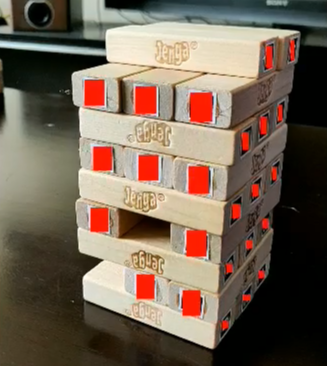
\includegraphics[width=\textwidth]{images/implementation/detection.png}
    \label{fig:detectedmarkers}
\end{minipage}\hfill
\begin{minipage}{.45\textwidth}
    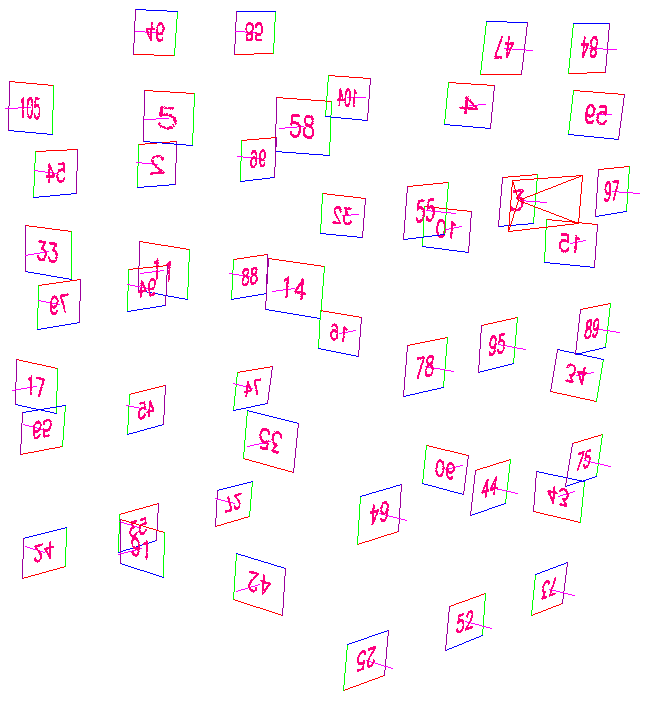
\includegraphics[width=\textwidth]{images/implementation/map}
    \label{fig:markermap}
\end{minipage}
\caption{Detected markers on image (left) and a constructed marker map (right)}
\label{fig:markersandmap}
\end{figure}

During the time that the user is scanning the tower, the client is sending images to the server whenever a new component is created, or an existing component is updated. Smartphone cameras generally capture around 30 frames per second, the majority of these frames will not contain any new information about the tower, so it makes sense to only send a subset of these images. Also, sending fewer images is more efficient and requires fewer resources from the client. Once the server has received all the images, it runs the MarkerMapper program with the camera calibration file it received earlier. The results of this can be seen in \cref{fig:markersandmap}.

The change from using UcoSLAM to using MarkerMapper was not unfounded. Advantages of using UcoSLAM were clearly defined in \cref{subsec:aruco}, however when implemented into the system UcoSLAM failed to perform to a satisfactory standard. For instance, the library resulted in segmentation faults depending on the order and content of images it processed, this means that sometimes UcoSLAM failed to produce a map of key points and markers. Clearly, this makes the library unacceptable for use at this time, however, it could quite easily be incorporated if it improves in the future. MarkerMapper is an older library that UcoSLAM was conceived from, and although it hasn't received any updates in over two years, it was able to produce a marker map with consistency, hence it is used throughout the rest of the project.
    
\section{\analysis}

\subsection{Reconstruction}

From the marker map produced earlier, a scene is built in Unity  (\cref{fig:reconstructionunity}. Marker maps are stored in the YAML 1.0 format (\cite{yaml}), which is long outdated, and while there are several YAML 1.2 libraries for deserialisation, there don't appear to be any libraries that support deserialisation for 1.0, so a short function was written to extract the relevant data and dump it into a C\# hashtable. The deserialisation task involves reading the file into a stream, splitting the stream up by certain vital characters, i.e. \{, [, :, and exporting the extracted coordinates with their corresponding marker id. These coordinates represent the three-dimensional location of the four corners of each marker.

\begin{figure}[ht]
    \centering
    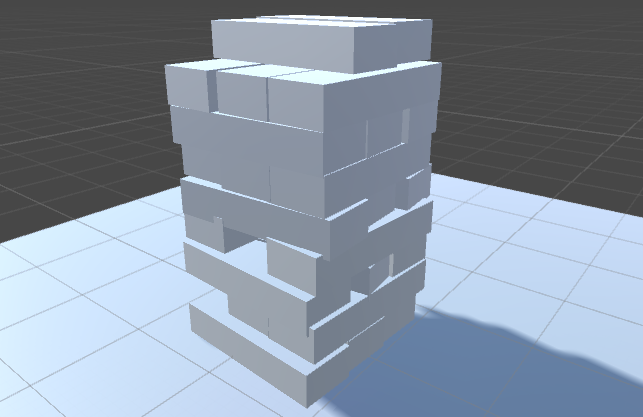
\includegraphics[width=\textwidth]{images/implementation/reconstruction}
    \caption{Reconstruction in Unity}
    \label{fig:reconstructionunity}
\end{figure}

Moving on, a Unity prefab was created to store the properties of virtual \jenga{} blocks. The dimensions of this object are variable, and can be set in the settings screen of the application, but by default, the object is set to 1.5x0.3x0.5 Unity units, this is because official \jenga{} blocks are of the same aspect ratio, and using units close to 1x1x1 makes development more manageable. Further, the object has a rigid body component attached to it, which means that the physics engine can control it, thus allowing it to be affected by collisions and gravity.

In order to instantiate the block GameObject, Unity requires a position, which indicates the centre point of the block, and a rotation, given as a Quaternion. It is clear that only knowing marker corner coordinates is not sufficient to instantiate the blocks; thus the centre point and rotation must be calculated. Finding the centre point of a block is straightforward; it involves finding the midpoint of each marker, and then finding the midpoint between those results. The algorithm used to find these midpoints can be seen in \cref{lst:midpoint}. Using midpoints of markers to calculate the centre of a block is an approximation, due to the placement of markers on real blocks being inconsistent, and also the detection and pose estimations having inaccuracies, which can cause generated objects to overlap, thus causing issues in analysis. However, it was found to be a sufficiently accurate approximation in most cases.

\lstinputlisting[style=cpp, linerange={341-344}, label={lst:midpoint}, caption={Calculating midpoints in \nameandsecref{codesec:analysis}}]{code/StandardTower.cs}

Further, a vector is calculated from the difference between the marker midpoints; this vector represents the direction that the block will be generated in. Also, for consistency, this directional vector, and the marker midpoints are all scaled to the size of the block prefab which was created earlier, thus finally allowing for the creation of the block objects. Afterwards, blocks are translated to the virtual origin so that the user can see them. Again, refer to \cref{fig:reconstructionunity} for an example of tower instantiation.

\subsection{Analysis}

Before the virtual tower can be used for analysis, its stability must first be assured; if the virtual tower were to fall over before any blocks are removed, then it would render the analysis useless. In some instances, the tower was found to sway on creation; this is because the model needs to adjust to the physics properties of the engine. To solve this motion problem, a function was devised which repeatedly waits for an in-game second, and then probes each block for information on its position and rotation, then when no blocks have moved since the last update, the tower is deemed settled;  \cref{lst:settling} shows how this algorithm was implemented in the code. Additionally, a maximum wait time of 10 seconds was decided, after which the tower is deemed to be unsettled, and the system will reject the tower state.

\lstinputlisting[style=cpp, linerange={185-193}, label={lst:settling}, caption={Waiting for settled tower in \nameandsecref{codesec:analysis}}]{code/StandardTower.cs}

Now, the removal feasibility rankings can be calculated. \cref{lst:analysis} shows that the implementation for this is quite short, yet effective. The process repeated is as follows: first, select the next block in the list and remove it, then, wait a specific amount of time, e.g. 5 seconds, next, get the sum of positional changes of every block, which is used as the score. To clean up, replace the block back into the tower and reset all blocks back to their original poses.

\lstinputlisting[style=cpp, linerange={279-293}, label={lst:analysis}, caption={Analysing removal feasibility in \nameandsecref{codesec:analysis}}]{code/StandardTower.cs}

Two key choices were made in the above implementation; how to remove the blocks, and how to calculate the score. As \citet{jengaanalysis} found, the various operations used to remove blocks from a tower affect neighbouring blocks in different ways, and that it is not possible to determine the effect that rotational moves make; for this reason, a simpler method was used, which involves simply deactivating the block in place. Furthermore, the score is calculated by finding the sum of distance travelled for each block, this works because it means moves which cause instability can be distinguished from moves that do not. It also results in a large score if the tower topples over, which is as expected.

Scores are then normalised and used to colour blocks on a scale between green and red, with green indicating ease of removal, and red the opposite. An example of this colouring can be seen in \cref{fig:analysisunity}, which shows the effectiveness of the analysis method deployed.

\vfill
\begin{figure}[ht]
    \centering
    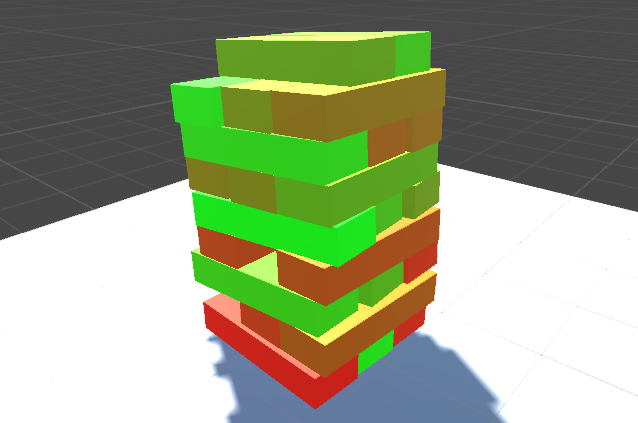
\includegraphics[width=\textwidth]{images/implementation/analysis}
    \caption{Block removal feasibility as a colour scale}
    \label{fig:analysisunity}
\end{figure}
\vfill

\section{\display}

After the scores for each block have been calculated, the next steps are to send the scores back to the client and display them. As discussed in \cref{sec:variantssummary}, the scores are displayed on a colour scale for aesthetic visualisation. This is achieved by detecting markers in each camera frame, and then drawing a box on top of each marker depending on their score. Since networking and detection functionality has already been implemented, the visualisation stage is easily attainable, requiring only normalisation of scores and drawing a filled, coloured rectangle using OpenCV. The resulting display is seen in \cref{fig:display}.

\vfill
\begin{figure}[ht]
    \centering
    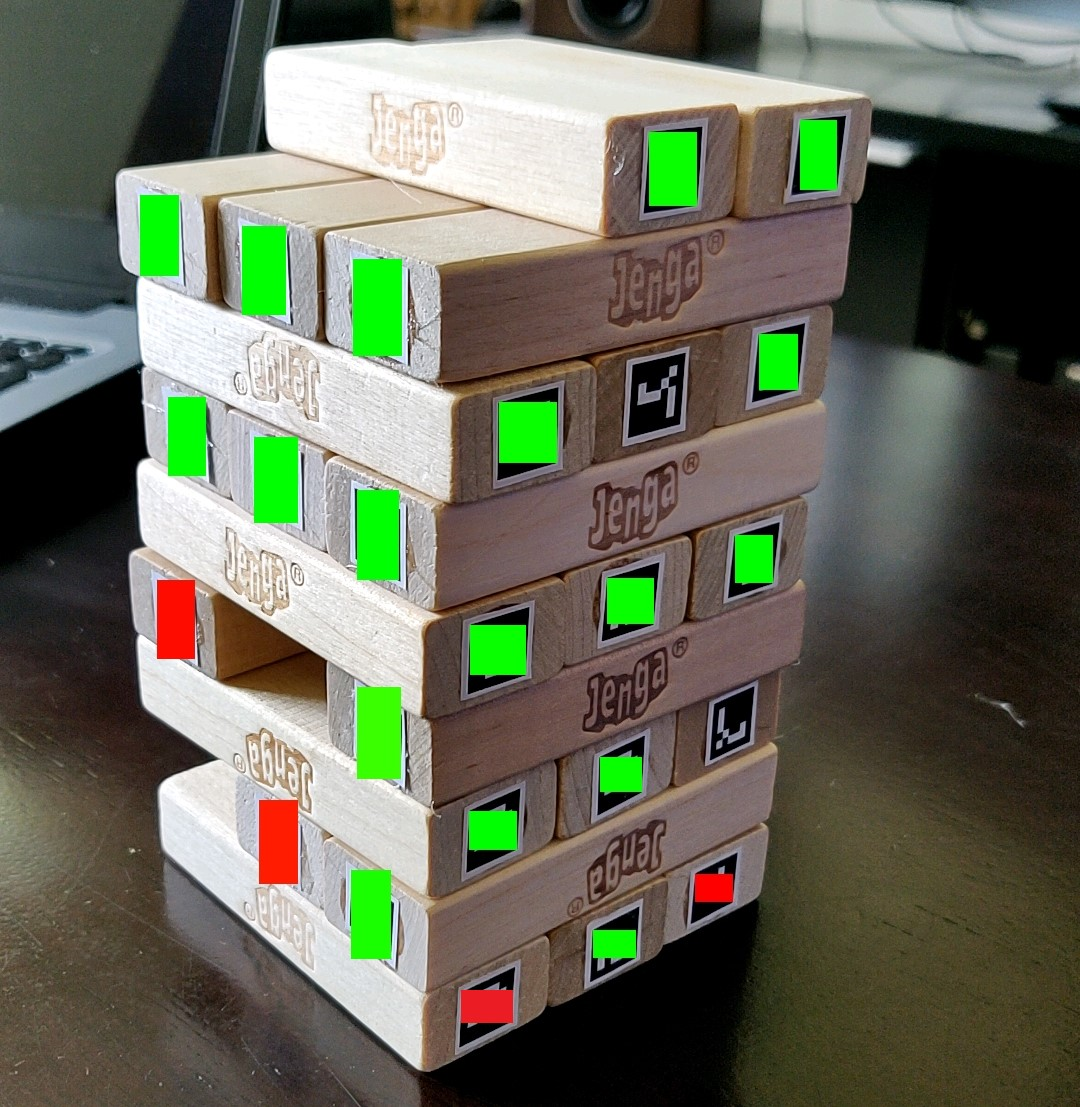
\includegraphics[width=.7\textwidth]{images/implementation/display}
    \caption{Visualisation of scores}
    \label{fig:display}
\end{figure}
\vfill

\newpage\section{Interfacing}

\begin{wrapfigure}{r}{5.5cm}
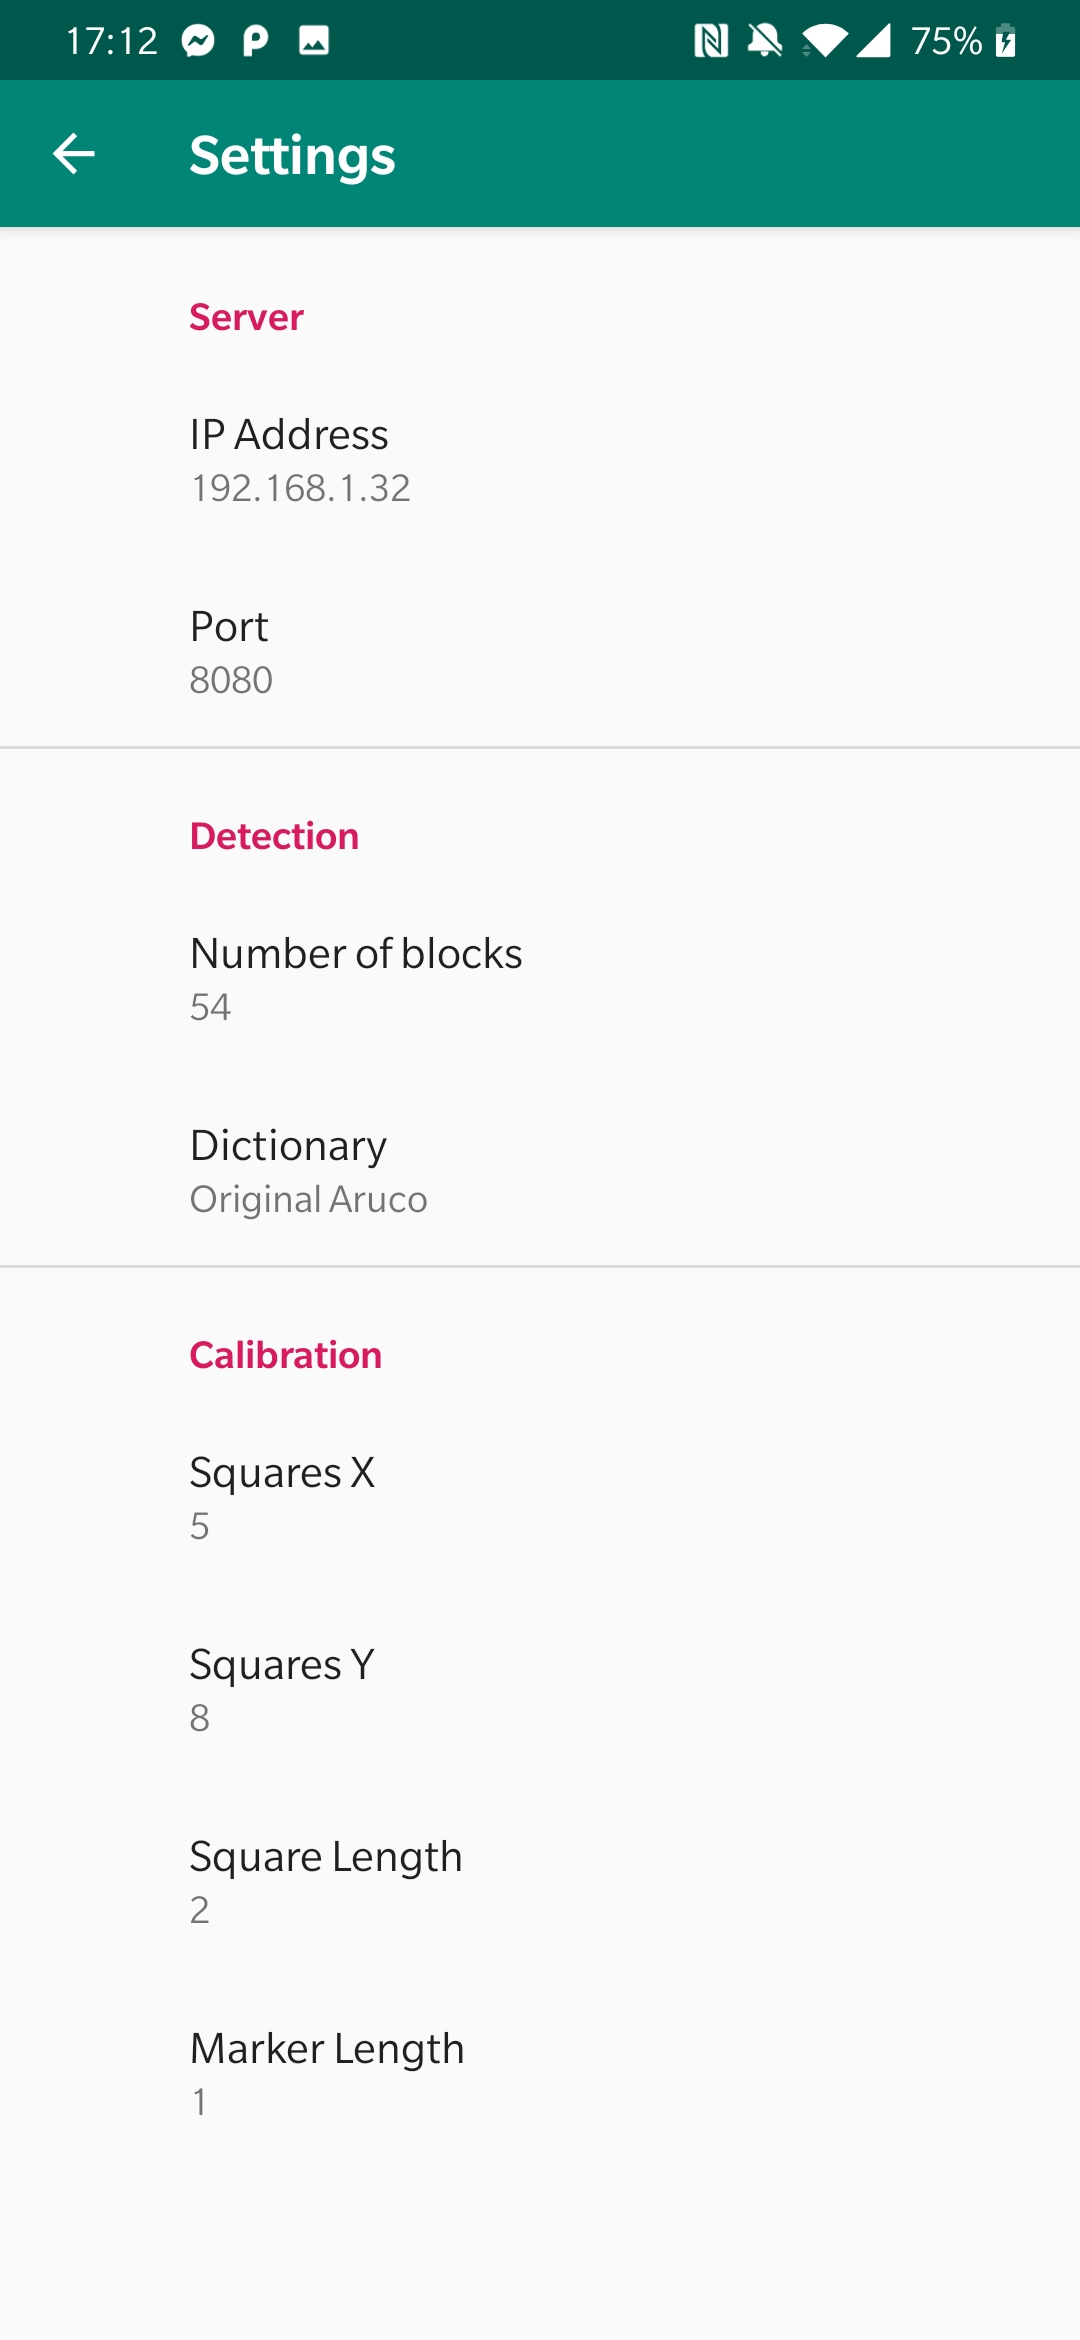
\includegraphics[width=4cm]{images/implementation/settings}
\caption{Settings screen}\label{fig:settings}
\end{wrapfigure}

When implementing the settings screen from the design section (\cref{sec:standalone}), it became clear of several drawbacks of the intended design. Firstly, the screen was missing some vital options, such as server address and port, and preferences for camera calibration. It is essential that these are included in the implementation because the server used by each user is likely to be running on a different address.

\cref{fig:settings} shows what the final implementation for the settings screen looks like. This design makes use of the Android preferences layout, which inflates a number of settings into a visually pleasing, scrolling window, which is better than previous iterations of design because of its consistency of layout and colour scheme. The previous design included a large button with which to enter the camera activity, but this was removed in favour of a back arrow, which conforms with the rest of the design for the settings.

\section{Additional GUI}

Whilst scanning the tower in to the system using fiducial markers has its benefits, it still requires the user to stick markers to both ends of each \jenga{} block, which is a monotonous task and therefore off-putting. Instead, an alternative was devised with which the user can build a virtual tower without the need for markers.

\cref{fig:towerbuilder} shows the different functionality that was implemented for such a system. When the user opens the application, they are greeted with an array of end and side blocks which appear to be in the shape of a tower. An effort was made to ensure these blocks looked realistic, in fact, the images used for the blocks were taken from a real set of \jenga{}, and then colourised and shaped to work with the application. Further, the user is able to zoom in and out, to see the full tower, or focus on a specific section for block removal. Or, the user can rotate the tower to view a different face.

The user is directed to tap on blocks in the application in the order that they were removed in the real tower; tapped blocks move from their position to the top of the tower, just as they would in the real game. By default, moved blocks go to the top left position, but can be moved to the centre, or top right, by simply clicking on them again.

While the tower is represented in a two-dimensional space, it retains a sense of realism due to the aesthetics of the blocks. This method for building the tower is beneficial because it is faster than the marker method, but its main drawback is that is doesn't account for rotation or translation of blocks; that is, blocks are assumed to be perfectly aligned in their position of the tower. Furthermore, this tower building activity was developed to be modular (\cref{req:modular}), which means that it is possible to swap out out the marker detection stage for this tower building activity, should the user choose to do so.

\begin{figure}[ht] % "[t!]" placement specifier just for this example

\hspace*{\fill}
\begin{subfigure}{0.22\textwidth}
\includegraphics[width=\linewidth]{images/implementation/build-start}
\caption{Start} \label{fig:buildstart}
\end{subfigure}
\hspace*{\fill}
\begin{subfigure}{0.22\textwidth}
\includegraphics[width=\linewidth]{images/implementation/build-zoom}
\caption{Zoom} \label{fig:buildzoom}
\end{subfigure}
\hspace*{\fill}
\begin{subfigure}{0.23\textwidth}
\includegraphics[width=\linewidth]{images/implementation/build-rotate}
\caption{Rotate} \label{fig:buildrotate}
\end{subfigure}
\hspace*{\fill}
\begin{subfigure}{0.22\textwidth}
\includegraphics[width=\linewidth]{images/implementation/build-end}
\caption{End} \label{fig:buildend}
\end{subfigure}
\hspace*{\fill}
\caption{Tower builder}
\label{fig:towerbuilder}
\end{figure}

\section{Summary}

The implementation chapter has shown how the system was implemented, from the development of networking functionality, through each stage of the project, leading to a working program that displays block removal feasibilities to the user. It also introduced an alternative for tower building, if the user does not want to attach markers to their blocks. For the sake of completeness, \cref{fig:pipeline} displays the whole pipeline of the project.

\begin{figure}[p] % "[t!]" placement specifier just for this example

\hspace*{\fill}
\begin{subfigure}{0.3\textwidth}
\includegraphics[angle=270,origin=c,width=\linewidth,keepaspectratio]{images/implementation/tower}
\caption{Tower state} \label{fig:a}
\end{subfigure}
\hspace*{\fill}
\begin{subfigure}{0.3\textwidth}
\includegraphics[width=\linewidth,keepaspectratio]{images/implementation/detection}
\caption{Detection} \label{fig:b}
\end{subfigure}
\hspace*{\fill}

\medskip

\hspace*{\fill}
\begin{subfigure}{0.3\textwidth}
\includegraphics[width=\linewidth,keepaspectratio]{images/implementation/map}
\caption{Marker map} \label{fig:c}
\end{subfigure}
\hspace*{\fill}
\begin{subfigure}{0.3\textwidth}
\includegraphics[width=\linewidth,keepaspectratio]{images/implementation/reconstructionportrait}
\caption{Reconstruction} \label{fig:d}
\end{subfigure}
\hspace*{\fill}

\medskip

\hspace*{\fill}
\begin{subfigure}{0.3\textwidth}
\includegraphics[width=\linewidth,keepaspectratio]{images/implementation/analysisportrait}
\caption{Analysis} \label{fig:e}
\end{subfigure}
\hspace*{\fill}
\begin{subfigure}{0.3\textwidth}
\includegraphics[width=\linewidth,height=200pt,keepaspectratio]{images/implementation/display}
\caption{Visualisation} \label{fig:f}
\end{subfigure}
\hspace*{\fill}

\caption{System pipeline} \label{fig:pipeline}
\end{figure}
%---=---==---===---====---=====---======---=====---====---===---==---=---%
%-                            SYSTEM TESTING                            -%
%---=---==---===---====---=====---======---=====---====---===---==---=---%

\chapter{Evaluation}\label{chap:evaluation}

Now that everything is implemented, an evaluation of the work is to be completed. This evaluation includes testing, discussions into objectives, literature and requirements, as well a summary for future work.

\section{Testing}

Testing in this project was not able to be extensive due to the large scope covered in research, design and implementation, as well as the limited time available. However, tests that were completed include unit tests and walk-through tests, which follow.

\subsection{Unit Tests}\label{unit}

Unit tests were written for ensuring that the view model for the tower builder application worked as intended, the code for this can be found in \cref{code:unittests}, these unit tests covered two main functions responsible for the addition of blocks to the tower.

Focusing on the \textit{addBlocksTest} class, there are 5 tests and a setup function, which creates the environment with which to test. Further, tests were created logically from the set of possible additions to the tower; no blocks, full row, single block, half full row, and overfull row. Each test includes an assertion which validates the number of blocks on the top row of the tower, for instance, adding 4 blocks to a tower that has a maximum row size of 3, would result in 3 blocks on the first row, and 1 on the top. These tests are necessary because they confirm the functionality of the system, and also serve as an aid when updating or improving the methods.

\begin{figure}[ht]
\hspace*{\fill}
\begin{subfigure}{0.3\textwidth}
\includegraphics[width=\linewidth]{images/evaluation/uibug.jpg}
\caption{New row bug} \label{fig:uibug1}
\end{subfigure}
\hspace*{\fill}
\begin{subfigure}{0.3\textwidth}
\includegraphics[width=\linewidth]{images/evaluation/uibug2.jpg}
\caption{Side block bug} \label{fig:uibug2}
\end{subfigure}
\hspace*{\fill}
\begin{subfigure}{0.3\textwidth}
\includegraphics[width=\linewidth]{images/evaluation/uibug3.jpg}
\caption{Size bug} \label{fig:uibug3}
\end{subfigure}
\hspace*{\fill}
\caption{Tower Builder Bugs}
\label{fig:uibugs}
\end{figure}

A few game breaking bugs were found during the development of the tower builder application, shown in \cref{fig:uibugs}. The unit tests written for the view model aided in the solution to these bugs because they were able to validate the soundness of the logic behind the application. In the case of the new row bug, the unit tests failed, determining that the interface was not the point of failure, after fixes were made to the code logic, the bug was solved. Furthermore, the tests were run when the side block bug and size bugs were identified, and it was determined that the code base was functional, meaning that the of the bugs were isolated to the tower drawing class, and were later fixed.

While unit tests are clearly beneficial, it takes a substantial amount of time to obtain full code coverage. Also, although automated interface testing is possible, it was not completed in this project due to time constraints, instead, manual visual feedback was necessary.

\subsection{Detection/Visualisation}\label{det}

Both the detection and visualisation stages same code base, and utilise the same layout, for this reason, it is sufficient to group them up for testing. As can be seen in the video demonstration (\cref{fig:demoqr}), both these stages have issues detecting all markers currently in a frame; while this is not necessary, it is visually displeasing to see markers without the expected augmentation. To fix this, the camera parameters for marker detection could be changed, but this would require to be set up for every different environment, and thus would need to be variable and added to the settings for each user to modify to work with their needs.

\subsection{Analysis}\label{blockapproximation}

Moving forward, the analysis stage was tested thoroughly, examples of this can be found in \cref{chap:results}. A critical issue that was identified in this testing was that blocks would occasionally be generated in the wrong place, this is due to inaccuracies in either: detection and pose estimation of markers, marker localisation and mapping, or approximation of centre point and rotation of blocks.

However, inaccurate block generation was only an issue in certain cases, for instance, when mapping a large number of blocks, i.e. all 54. It was determined that the cause of the error was in the detection stage, and occurred when a large number of markers were shown in a single frame. With there being a large number of markers, it seems that errors are increased in pose estimation. To solve this problem, multiple images per face need to be taken, and so the implementation should be changed to accommodate for this.

On occasion, the reconstruction would be accurate, but then the tower would fall over before any blocks were removed. This is due to some of the blocks overlapping, thus generating large amounts of force inside the tower, causing the blocks to be pushed outwards. The fact that this issue did not occur in every test suggests that again it is a problem with the detection stage, with blocks being detected in slightly the wrong places. Again, this can be solved by holding the camera closer to the tower, thus detecting fewer markers per frame.

\begin{figure}[ht]
    \centering
    \includegraphics[width=.7\linewidth]{images/testing/smallgame2.jpg}
    \caption{A reconstruction that toppled over before analysis could begin}
    \label{fig:unsettled}
\end{figure}



Moreover, when a virtual tower was reconstructed successfully, the analysis was accurate; blocks marked red were clearly difficult to remove, and green blocks were clearly easy to remove. Although layers near to the top of the tower are out of bounds during the game, due to them being easier to remove, it is still worthwhile to show their removal feasibility to the user for completeness.

\section{Attaining Objectives}

With testing complete, the evaluation moves on to the objectives set at the beginning of the project. This short section shows how all objectives were attained by the end of the time frame of the project.

\hyperref[obj:detect]{Objective 1} was achieved through the use of square planar markers and the ArUco library. This detection method is robust to rotational and translational differences in blocks, and can, therefore, be used in any real-world scenario, unlike competing methods.

Also, \hyperref[obj:analysis]{Objective 2} was reached through the use of the MarkerMapper application, which was able to localise and map the detected markers. The marker map gained was then used to reconstruct the tower in Unity, which was analysed using a state-of-the-art simulation method.

Finally, \hyperref[obj:display]{Objective 3} was accomplished by using a combination of OpenCV and ArUco. Scores sent from the analysis stage were normalised and converted into colours on a green to red scale, which were then successfully displayed to the user, thus completing the system.

\section{Use of Literature}

The \nameandsecref{chap:background} was a substantial part of this project, this section aims to show how the knowledge gained in the literature and technology review was used to aid in the development of the system.

Firstly, the \nameandsecref{sec:reconstruction} looked into the various methods for reconstruction and determined that the most appropriate category was parts-based, and also found that voxel-based and view-based modelling were not sufficient for use in the project. This meant that the project should build the virtual tower from a library of block objects, which subsequently lead to the creation of a Unity GameObject that was used in the creation of virtual blocks.

Secondly, the review of the previous \jenga{} analysis papers showed the various ways in which towers could be analysed for block removal feasibility; namely, \citet{jengarobot} used a simulation method which was the inspiration for the analysis method used in this paper.

Finally, the research into augmented reality SDKs and libraries (\cref{sec:markerbased}) was beneficial because it gave knowledge about the current state of AR, and also identified that MarkerMapper and UcoSLAM were the most appropriate libraries for use in this project, coincidentally MarkerMapper became a crucial part of the reconstruction stage.

\section{Meeting Requirements}

Now that the objectives have been shown to be met, and the use of literature has been established, naturally this section progresses into the state of requirements, and giving reasons as to why certain requirements were or were not met. As there are a couple dozen requirements set for this project, it was deemed worthwhile to only discuss a subset of them in this section, however, a full list of requirements and their statuses can be found in \nameandsecref{chap:requirements}.

To begin with, \cref{req:towerstate} states that the system could be able to detect when the tower has changed state. This requirement was not met because knowledge of the tower is based on a full set of images around its perimeter, meaning that for the system to know whether the tower has changed state, the user would have to essentially run through the whole detection stage, which is done by the user when they want a new analysis anyway.

Further, \cref{req:inaccuracies} was not met because accounting for inaccuracies in pose estimation would require a significant amount of testing and work, that simply didn't fit into the time frame or scope of the project. However, due to the project being maintainable (\cref{req:maintainable}), future work could be done to solve the inaccuracy problem.

The project does not use multiple analysis techniques, which violates \cref{req:multianalysis}. This was decided because of the many possibilities of tower state, meaning that a rule-based analysis would be inaccurate. However, the simulation method provides a robust analysis which takes around 5 seconds for reasonably sized towers, so using this as the sole way to analyse the tower is dignified.

A final note can be made towards the \cref{sec:req:additional} of requirements, which were added part way through the project. This change in requirements was due to library compilation issues, and subsequently caused a lot more work than was initially required for system completion. This increase of scope reduced the amount of time available to spend on other stages of the project, but it was worth the effort because it formed the basis of communication, and allowed for the separation of complexity between server and client.

\section{Future Work}

The final section in this evaluation chapter opens a discussion into the future progression of the project, after the end of the planned time plan. It begins with extensions and maintenance of the system, then does into commercial potential, and finally shows how the system can be used outside of the game of \jenga{}.

\subsection{Extension}

Extensions to the project are endless, ranging from improving the interface, to adding extra techniques and methods. This section aims to identify the most plausible and worthwhile extensions that should be considered when extending the system. Also, with the project being modular (\cref{req:modular}) the complexity of incorporating the following extensions is decreased, when compared with a project that is not built to be modular.

The first extension that comes to mind is the addition of machine learning (ML) into the analysis stage, this is because, as described in \cref{subsec:machinelearning}, ML would fit well into the system. Doing so would potentially increase the accuracy and also decrease the time taken for analysis.

Furthermore, ARCore (\cref{sec:arcore}) would improve the visualisation stage considerably. Currently, OpenCV is used for the display of scores on blocks by drawing filled rectangles in place, but using ARCore the system would be able to display a full tower in a multitude of ways. Particularly, the model reconstructed in Unity could be used to visualise a virtual tower in such a way that it stands next to the real tower, or even overlay the tower completely; this would allow for a more immersive user experience.

Finally, it seems reasonable to suggest that the variants, conceived in \cref{subsec:variation}, should be included in the next release of the system; due to their increase of gamification and thus ability to keep the attention of the user (\cref{req:attention}). The most favoured of which is the challenges variant, this is because players of the game commonly draw on their tower pieces to add challenges, but this gives rise to a problem; more specifically the permanence of writing on blocks means that users cannot change nor remove the challenges. Using augmented reality to add challenges would solve this problem.

\subsection{Commercial Potential}

As well as the numerous possible extensions, this system proposed by this paper has significant commercial potential. For this project to become commercially viable, it should become self-contained (\cref{req:selfcontained}), this would be possible by fixing the compilation issues with MarkerMapper, or developing a marker mapping solution without use of the library. Given this, the system would be able to be deployed to a standalone Android app, and thus make it more accessible to consumers.

Further, the system requires markers to be affixed to blocks; this is a lengthy task which is off-putting to users. However, there are several companies that offer custom printed labels, which could be used to print off AR markers as stickers, thus providing a simpler way to set up the system and also reducing the time spent doing so.

\subsection{External Applications}

The final section in this evaluation describes the possible applications of the system outside the game of \jenga{}, most notably in structural analysis. An example of a possible structure and its analysis can be seen in \cref{fig:structureanalysis}; it shows that the system, without modification, can properly analyse the integrity of a structure, provided markers can be affixed. The analysis shows that the parts towards the lower end are vital to its integrity, and would cause more damage to the structure if they were removed, than the parts at the top.

\begin{figure}[ht]
    \hspace*{\fill}
    \begin{subfigure}{0.3\textwidth}
    \includegraphics[width=\linewidth]{images/testing/structure-real.jpg}
    \caption{Possible structure} \label{fig:structure}
    \end{subfigure}
    \hspace*{\fill}
    \begin{subfigure}{0.5\textwidth}
    \includegraphics[width=\linewidth]{images/testing/structure.jpg}
    \caption{Structural analysis} \label{fig:structureanalysis}
    \end{subfigure}
    \hspace*{\fill}
\end{figure}

%---=---==---===---====---=====---======---=====---====---===---==---=---%
%-                             CONCLUSIONS                              -%
%---=---==---===---====---=====---======---=====---====---===---==---=---%

\chapter{Conclusion}\label{chap:conclusions}
This project has provided a method which is robust to real-world problems, such as the randomness of block translations and rotations created on each player turn, unlike other work in the area, specifically the popular \jenga{} robot described by \citet{jengarobot}. It also makes use of augmented reality which grants the system serious market potential, given the modern day rise of AR systems.

There are several problems with the current state of the system, such as with block approximation, discussed in \cref{blockapproximation}, marker detection (\cref{det}), and low unit test coverage (\cref{unit}), which could all be improved in the continuation of the project, given the state of modularity and maintainability of the system. 

One aspect that could certainly have been worked on more effectively is project scope. I found myself having an ever-growing amount of work throughout the project, namely research and attempted implementation of UcoSLAM, a localisation and mapping method proposed in a paper earlier this year \citep{ucoslampaper}. I feel that if the amount of time spent using this emergent solution was used elsewhere in the project, such as the implementation of the visualisation stage, then the system would be substantially stronger and would better display the market potential of the method.

Despite all this, I am happy with the project as a whole, because I reached all the objectives set in \cref{objectives}, and provided a working system and clear proof of concept of a novel method. Furthermore, the system is built in a maintainable and extendable manner, which means that the project can be picked up by another student or like-minded individual who wishes to progress the knowledge and methods in the area.

\bibliography{Bibliography}

\appendix
%---=---==---===---====---=====---======---=====---====---===---==---=---%
%-         REQUIREMENTS ANALYSIS AND REQUIREMENTS SPECIFICATION         -%
%---=---==---===---====---=====---======---=====---====---===---==---=---%

\chapter{Requirements}\label{chap:requirements}

This chapter focuses on project requirements. It begins with an explanation of the process of requirements \nameandsecref{sec:requirementscapture} and analysis, continues with a discussion of crucial \nameandsecref{sec:requirements} and areas of particular challenge, and then ends with addressing, with prudence, the issue of project \nameandsecref{sec:scope}.

\section{Capture} \label{sec:requirementscapture}

Requirements are an essential aspect of any project, as they formulate the purpose of the software, and set clear goals. Without requirements, developers may lose sight of what needs completing, and so may fail to deliver as expected; it would also cause problems in testing, as testers would be unable to refer to how an application should function. A keen effort was made to develop specific requirements, with low ambiguity, and written concisely.

In this project, the requirements were captured from the \nameandsecref{chap:background}, through research and technology review. Relevant academic papers were evaluated to ascertain what is possible to develop using current state-of-the-art methods, and these are reflected on in the requirements. Also, technology was reviewed to determine what had gone well, not so well, and what to avoid doing from previous projects.

Another method used for requirements capture was the short coding exercise in \cref{subsec:hough}, which was key to the capture process. Short coding can quickly validate a method before allotting it a more substantial amount of time, in this case, time was saved by determining that using markerless detection methods; specifically, the Hough-Lines transform, was infeasible.

\section{Requirements} \label{sec:requirements}

Using the techniques discussed previously in \cref{sec:requirementscapture}, this section aims to formulate requirements in response to the problems identified in \cref{sec:challenges}. It opens a discussion into the critical requirements in each stage of the system, explains why they were chosen and focuses on areas of particular challenge, difficulty or conflict. The full breakdown of requirements can be found in \cref{app:requirements}.

\subsection{\detection}



As was summarised in \cref{subsec:detectionsummary}, the system should use marker-based detection methods because of its clear advantages over markerless detection. Namely, it allows for an immediate understanding of object poses without the need for further analysis. Another reason to use marker based detection is that if a marker is detected, then it is known that a block exists at that location, meaning that it implicitly meets \cref{req:blocknonblock,req:tower}, which would otherwise require explicit solving.

Moreover, UcoSLAM is a library well fit for this project, due to its ability to map the locations of both markers and key points, thus gaining a deeper understanding of the environment, and so it should be adopted as the method of choice.

\subsubsection{Pose Estimation}\label{subsec:poseestimation}

There are a few options to consider for how to employ marker-based detection with a \jenga{} tower, in particular, answering the question of which block faces should markers be affixed. Firstly, affixing markers to every face would be a viable solution, as it means every block face can be identified and have its pose estimated; however, this solution involves a high setup time cost, and it also requires a larger dictionary of markers. Using a larger dictionary is disadvantageous because it means that the detection algorithm needs to search for more markers, thus increasing detection time, and also resulting in a higher chance for errors, i.e. false positives \citep{ucoslampaper}.

The opposite of the above solution is only to use one marker per block, which is better because it has less setup time, and requires a smaller dictionary size. If a single marker is attached to an end face of a block, then after estimating its pose, the full block pose can be estimated by using known dimensions, which in the official game are 15mm x 25mm x 75mm. On first look, this solution seems like it would be successful, although the faces are small, and markers will have to be even smaller, as there needs to be a relatively small amount of whitespace around each marker so that the detection algorithm does not confuse multiple markers as being part of one. Also, small markers are subject to pose ambiguity, as shown in \cref{fig:poseambiguity}, so although a marker pose estimations may be incorrect.

\begin{figure}[ht]
\begin{minipage}{\textwidth}
    \centering
    \includegraphics{images/requirements/ambiguity_problem.png}
    \caption{The ambiguity problem, image from the \protect\footurl{https://docs.google.com/document/d/1QU9KoBtjSM2kF6ITOjQ76xqL7H0TEtXriJX5kwi9Kgc}{ArUco Documentation}}
    \label{fig:poseambiguity}
\end{minipage}
\end{figure}

The ArUco library tries to solve the ambiguity itself, by using various error correction methods, but there is a way to can solve the ambiguity problem with \jenga{} pieces; that is affixing a marker to both end faces of each block. This eliminates the problem by estimating the position and orientation of both markers for a tower piece, and then reconstructing the piece to be between the two markers. In fact, this method means that the pose of each marker can be discarded, as only their relative locations are required for reconstruction.

\subsubsection{Camera}

A problem that comes with marker-based detection is camera distortion, which is common with modern cameras. Distortion is a problem because it means that two separate cameras could look at the same environment and come to a different understanding. As this project plans to solve the block removal problem in a real-world environment, as opposed to a lab-style fixed-camera environment as in previous solutions, this solution must account for camera-specific distortion, which brings about the need for \cref{req:camera}.

\begin{figure}[ht]
\begin{minipage}{\textwidth}
    \centering
    \includegraphics[width=.6\textwidth]{images/requirements/camera-distortion.jpg}
    \caption{Camera distortion, image from \protect\footurl{https://clickitupanotch.com/lens-distortion/}{Click it up a Notch}}
    \label{fig:cameradistortion}
\end{minipage}
\end{figure}

Another critical requirement is that the detection stage must be able to send the information it acquires about the block poses to the analysis stage, this is because a working system must have communication between its components; otherwise, it is not a single system, but a sum of separate components. Also, the stages may be written in different languages, so communication should be language independent. The requirements for the analysis stage are described next.

\subsection{\analysis}

\cref{sec:categoriessummary} identified that the most appropriate category for modelling a \jenga{} tower is parts-based. Marker-based detection compliments part-based modelling because a virtual block can easily be created between two markers, whereas other types of modelling would require more work to reach the same outcome.

\subsubsection{Reconstruction}
The marker map gained from the detection stage can be used to reconstruct the tower (\cref{req:reconstruct}), this needs to be done in such a way that the initial virtual tower remains stable if its real-world equivalent is also stable. However, there may be inaccuracies in the marker map, which presents the problem in physics simulations that some blocks may overlap when built solely from the positions in the marker map. To solve this, the system must account for pose estimation inaccuracies, which brings about \cref{req:inaccuracies}. It is worth noting that this would not be a problem with heuristic analysis because the analysis is less advanced and exact block poses are not required.

\subsubsection{Ranking}
In \cref{sec:problem}, it was introduced that the main problem faced by \jenga{} players is deciding which block to remove (\cref{req:rank}). This has been addressed in several papers, as researched in \cref{sec:structuralanalysis}, with some opting for a heuristic analysis, and others a physics analysis.

A heuristic analysis involves the creation of a set of rules which determine how likely is it for the tower to fall after removing a block. Applying such a rule set to a tower state is fast, and can therefore be performed in real time. While the rule set is unlikely to contain rules that users cannot think of themselves, this method provides an immediate analysis of all blocks (\cref{req:realtime}), which users cannot do. A significant drawback to this type of analysis is that it only takes into account a few physical constraints, such as pivoting, but misses more complex physics factors like weight distribution and friction.

On the other hand, physics simulation, if done correctly, can accurately represent a real-world tower in a virtual environment, accounting for several more physics factors than the heuristic approach. Using such an approach would therefore result in a more accurate analysis, which would be more beneficial to the user, however, it would also take more time. It is favourable to allow the user to choose between these two approaches (\cref{req:multianalysis}), as they both have advantages over the other.

\subsection{\display}

Following on from the analysis stage, it is vital for the system to display the analysis results (\cref{req:display}). This can be achieved in various ways, but as discussed in the \nameandsecref{sec:motivation}, there is significant market potential in augmented reality, and so the system should show the analysis using this technology.

\subsection{System}

Finally, there is a set of requirements for the system itself, two of which that are key are being easy to understand (\cref{req:understand}) and keeping the attention of the user (\cref{req:attention}), this is because if the user does not know how to use the system, or loses interest, then they are usually only one tap away from closing the application and doing something else.

Furthermore, there are high priority requirements which focus on how the software is to be written. For instance, \cref{req:selfcontained,req:modular} describe that the system should be self-contained, meaning the user should be kept within the system when using the different stages, but also modular, to keep these stages programmatically separate for the means of maintainability (\cref{req:maintainable}) and extensibility (\cref{req:extendable}).

\section{Scope}\label{sec:scope}

This project spans over about seven months and includes much research and planning, followed by designs and extensive implementation. Testing is also a requirement for the project, without which the viability of the system would be unconfirmed. With such a short amount of time to complete the project, it is important for the scope to be adequately defined.

Moreover, the possibilities for this project are limitless, as it can be expanded in almost every direction. For example, current state-of-the-art methods for the detection of block poses go into significant detail, and would require months of research and development find or improve upon alone. Yet, this is only one of the three main stages to be completed in this project, and time must be divided up fairly between them.

It would have been useful to incorporate machine learning into both the detection, as advanced object classification, and the analysis stage, as an advanced prediction method. The machine learning method has the potential to be both accurate, and fast, in the analysis of block removal feasibility, making it more favourable than the heuristic and physics simulation options. However, this method was descoped because, without prior experience with machine learning techniques, it had the potential to engulf the rest of the project.

Further, augmented reality is an ever-growing field in Computer Science, and so new techniques are often created, which can be a problem. For instance, the latest technologies may not be as stable or clear to use as the less recent, well-documented alternatives. Also, a difficult decision arises if part way through the project a new technique was released that would seem to solve a problem in a better way than the technology found during research, due to pressing time constraints.

UcoSLAM, the library that will be used for block detection, is so cutting edge in its field that the paper describing its approach was only released in February of this year. Deciding to use the library so late in the project was not straightforward because although it appeared to be able to solve the block detection problem, there would be little support with development. Changing the scope to include UcoSLAM also reduced the amount of time available for design and implementation, but was deemed necessary due to the functionality it provided.

\section{Summary}

To summarise, this section has defined the functional and non-functional requirements for each stage of the system, as well as the system as a whole. The next chapter uses these requirements as the basis for system design.
\chapter{Contribution}\label{chap:contributing}

\section{OpenCV}

When learning how to find straight lines in images using OpenCV, I found mistakes in the Hough Lines Transform tutorial code. Two sets of code contained logical errors which resulted in only one line being drawn, from a set of multiple detected lines. The code snippets below demonstrate how I was able to fix these bugs, or you can view the currently open pull request on GitHub here: \url{https://github.com/opencv/opencv/pull/14391}.

\vfill
\begin{multicols}{2}
\begin{lstlisting}[style=python,caption={Hough Lines tutorial code}]
lines = cv.HoughLines(...)
for line in lines:
    rho,theta = line[0]
    ...
\end{lstlisting}
\begin{lstlisting}[style=python,caption={Fixed array indexing bug}]
lines = cv.HoughLines(...)
for line in lines[0]:
    rho,theta = line
    ...
\end{lstlisting}
\end{multicols}

\begin{multicols}{2}
\begin{lstlisting}[style=python,caption={Hough Lines P tutorial code}]
lines = cv.HoughLinesP(...)
for line in lines:
    x1,y1,x2,y2 = line[0]
    ...
\end{lstlisting}
\begin{lstlisting}[style=python,caption={Fixed array indexing bug}]
lines = cv.HoughLinesP(...)
for line in lines[0]:
    x1,y1,x2,y2 = line
    ...
\end{lstlisting}
\end{multicols}
\vfill
\newpage
\section{ArUco}

Further, ArUco is a requirement for when compiling MarkerMapper, yet CMake fails when attempting to compile MarkerMapper with the only available version of ArUco (3.1.0). Initially I thought this was due to MarkerMapper not being maintained, but thorough evaluation of the ArUco code found it was missing the implementation of a detection function. The declaration for the function exists in a header file, shown below:

\begin{lstlisting}[style=cpp,caption={Declaration of function in ArUco markerdetector.h}]
void detect(const cv::Mat& input, std::vector<Marker>& detectedMarkers, cv::Mat camMatrix = cv::Mat(), cv::Mat distCoeff = cv::Mat(), float markerSizeMeters = -1, bool setYPerperdicular = false);
\end{lstlisting}

But I had to implement the function definition myself, which is as follows:

\begin{lstlisting}[style=cpp,caption={Added function definition}]
void MarkerDetector::detect(const cv::Mat& input, std::vector<Marker>& detectedMarkers, cv::Mat camMatrix, cv::Mat distCoeff, float markerSizeMeters, bool setYPerpendicular)
{
    _impl->detect(input, detectedMarkers, camMatrix, distCoeff, markerSizeMeters, setYPerpendicular);
}
\end{lstlisting}

As ArUco is not hosted on any kind of version control system, like GitHub, I was unable to create a pull request with the changes, however, the developers have been made aware of the bug, and it remains to be seen whether it will be fixed with the next release.
\chapter{Ethics}\label{chap:ethics}

\subsubsection{Have you prepared a briefing script for volunteers?}
Yes, the participants have been briefed on the brainstorm study. They have been made aware that the data they provide will be collected and used in this project for design capture.

\subsubsection{Will the participants be using any non-standard hardware?}
No, hardware includes a whiteboard and pen.

\subsubsection{Is there any intentional deception of the participants?}
No intential deception of the participants is planned.

\subsubsection{How will participants voluntarily give consent?}
Reponses by participants will be anonymous, and they will give verbal consent at the time of the study.

\subsubsection{Will the participants be exposed to any risks greater than those encountered in their normal work life?}
There is no greater risk exposed to participants in this study.

\subsubsection{Are you offering any incentive to the participants?}
There is no incentive given to the participants.

\subsubsection{Are any of your participants under the age of 16?}
All participants are over the age of 16.

\subsubsection{Do any of your participants have an impairment that will limit their understanding or communication?}
None of the participants have impairments.

\subsubsection{Are you in a position of authority or influence over any of your participants?}
I am not in a position of authority over the participants.

\subsubsection{Will the participants be informed that they could withdraw at anytime?}
Of course, the participants will be informed that they can withdraw at anytime.

\subsubsection{Will the participants be informed of your contact details?}
All participants will be able to contact me after the investigation, with the details provided to them after the study.

\subsubsection{Will participants be de-briefed?}
Students will be debriefed after the study to enable them to understand the nature of the investigation.

\subsubsection{Will the data collected from the participants be stored in an anonymous form?}
All data collected will be stored on a whiteboard, with no personal information attached, ensuring anonymity.
\chapter{Analysis Results}\label{chap:results}

\newcommand{\towerandanalysis}[2]{
    \hspace*{\fill}
    \begin{subfigure}{0.25\textwidth}
    \includegraphics[angle=270,origin=c,width=\linewidth]{images/testing/#1-real.jpg}
    \caption{#2 Tower} \label{test:#1real}
    \end{subfigure}
    \hspace*{\fill}
    \begin{subfigure}{0.65\textwidth}
    \includegraphics[width=\linewidth]{images/testing/#1.jpg}
    \caption{#2 Analysis} \label{test:#1}
    \end{subfigure}
    \hspace*{\fill}
}

\begin{figure}[ht]
\label{fig:tests}

\towerandanalysis{disorderly}{Disorderly}
\medskip
\towerandanalysis{game1}{Game 1}

\end{figure}
\begin{figure}[htb]\ContinuedFloat

\towerandanalysis{perturn1}{Turn Game 1}
\medskip
\towerandanalysis{perturn2}{Turn Game 2}
\medskip
\towerandanalysis{perturn3}{Turn Game 3}
\medskip
\towerandanalysis{perturn4}{Turn Game 4}

\end{figure}
\begin{figure}[htb]\ContinuedFloat

\towerandanalysis{perturn5}{Turn Game 5}
\medskip
\towerandanalysis{perturn6}{Turn Game 6}
\medskip
\towerandanalysis{smallgame1}{Small Game 1}
\medskip
\towerandanalysis{smallgame2}{Small Game 2}

\end{figure}
\begin{figure}[htb]\ContinuedFloat

\towerandanalysis{smallgame3}{Small Game 3}
\medskip
\towerandanalysis{smallgame4}{Small Game 4}
\medskip
\towerandanalysis{singlestack}{Single Stack}
\medskip
\towerandanalysis{structure}{Structure}

\end{figure}
\chapter{Code}\label{chap:code}

This chapter shows the most important code files that were created for this project. However, the full code base is available for viewing at my public GitHub repository by following \url{https://github.com/obroomhall/JengAR}, or by using the QR code displayed below. Each file shown in this document references the directory that it can be found in project files.

\vfill
\section{Code Structure}

\begin{table}[ht]
\centering
\begin{tabular}{l|l}
\textbf{Directory} & \textbf{Description} \\ \hline
\textbf{3rdparty} & A selection of third party libraries used in the project  \\
\textbf{android} & Android application  \\
\textbf{client} & Client files  \\
\textbf{extra} & Tower builder Android application  \\
\textbf{python} & Markerless detection application  \\
\textbf{server} & Server files  \\
\textbf{shared} & Header files used by Client and Server  \\
\textbf{unity} & Unity analysis program
\end{tabular}
\end{table}
\vfill

\begin{figure}[h]
    \centering
    \includegraphics[width=.5\linewidth]{images/code-qr}
    \caption{GitHub Code}
    \label{fig:githubqr}
\end{figure}

\newpage\minitoc

\lstset{basicstyle=\scriptsize}

\begin{landscape}
\begin{multicols}{2}

\section{Markerless Detection}
\subsection{hough.py}\label{code:houghpy}
Python program for finding straight lines in an image using the probabilistic hough transform with OpenCV. Located in \textbf{python/}.
\texttt{\lstinputlisting[style=python]{code/hough.py}}

\section{Networking}\label{codesec:network}
\subsection{network.hpp}\label{code:network}
Superclass used to define various networking functions for use in the Server and Client subclasses. Located in \textbf{shared/include/jengar/}.
\texttt{\lstinputlisting[style=cpp]{code/network.hpp}}

\section{Detection}\label{codesec:detection}

\subsection{dictionary.cpp}\label{code:dictionary}
This class is mainly used for converting ::aruco::Dictionary types to cv::aruco::Dictionary types. Located in \textbf{server/src/}.
\texttt{\lstinputlisting[style=cpp]{code/dictionary.cpp}}

\subsection{native-lib.cpp}\label{code:native}
JNI class which allows the Android client to use this projects native C++ code. Located in \textbf{android/app/src/main/cpp/}.
\texttt{\lstinputlisting[style=cpp]{code/native-lib.cpp}}

\section{Analysis}\label{codesec:analysis}
Unity script that builds a tower from a marker map, analyses block removal feasibility, and then saves the results to a .csv file. Located in \textbf{unity/Assets/}.
\texttt{\lstinputlisting[style=cpp]{code/StandardTower.cs}}

\section{Extra}\label{codesec:extra}

\subsection{BuildViewModel.java}
View model for the tower builder activity, handles the logic behind how blocks are moved within the tower, and sends information to the BuildFragment for display. Located in \textbf{extra/app/src/main/java/com/example/jengar/ui/main}.
\texttt{\lstinputlisting[style=java]{code/BuildViewModel.java}}

\subsection{BuildViewModelTest.java}\label{code:unittests}
JUnit tests for the tower builder view model. Located in \textbf{extra/app/src/test/java/com/example/jengar/ui/main}.
\texttt{\lstinputlisting[style=java]{code/BuildViewModelTest.java}}

\end{multicols}
\end{landscape}

\end{document}
